\documentclass[plainsections,alongposter]{sciposterlocal}

\usepackage{multicol}
\usepackage{mathpazo} % Better fonts
\usepackage{parskip}
\usepackage{amsmath}
\usepackage{booktabs}
\usepackage[utf8]{inputenc}
\usepackage{graphicx}
\usepackage[np]{numprint}
\usepackage{tikz}
\usepackage{gnuplot-lua-tikz}
%\usepackage{lineno}
%\linenumbers

%
% Macros
%
\newcommand{\tr}{\rm{Tr}}
\newcommand{\mean}[1]{\left\langle{#1}\right\rangle}
\newcommand{\comment}[1]{{\bf\textit{#1}}}

%%%%%%%%%%%% Header info
\title{The QCD phase-diagram obtained from the NJL and the extended-NJL models for quark and hadron phases}

\author{Clebson A. Graeff$^\dagger$; Débora P. Menezes$^*$}
\email{cgraeff@utfpr.edu.br, debora.p.m@ufsc.br}

\institute{$^\dagger$~Universidade Tecnológica Federal do Paraná -- Pato Branco, PR - Brazil \\
$^*$~Universidade Federal de Santa Catarina -- Florian\'opolis, SC - Brazil \\
}

\leftlogo{Logo_UTFPR_PB_cor.pdf}
\rightlogo{Brasao_UFSC_PDF.pdf}
%%%%%%%%%%%%

%%% Color for sections titles
\definecolor{SectionColor}{rgb}{0.22,0.33,0.6}

%%% Set roman fonts instead of sans serif
\renewcommand{\familydefault}{\rmdefault}

%%% No rules between columns, please
\setlength{\columnseprule}{0pt}

%%% BibTeX bibliography style
\bibliographystyle{plain}

%%%%%%%%%%%%%%%%%%%%
%%% The Document %%%
%%%%%%%%%%%%%%%%%%%%
\begin{document}

\maketitle % The Header

\begin{multicols}{2} % Start content area

%%%%%%%%%%%%%%%%%%%
\section*{Abstract}
{ \it
We analyse the hadron/quark phase transition described by the Nambu-Jona-Lasinio (NJL) model [quark phase] and the extended Nambu-Jona-Lasinio model (eNJL) [hadron phase]. While the original formulation of NJL model is not capable of describing hadronic properties due to its lack of confinement, it can be extended with a scalar-vector interaction so it exhibits this property, the so-called  eNJL model. As part of this analysis, we obtain the equations of state within the SU(2) versions of both models for the hadron and the quark phases and determine the binodal surface. 
}

%%%%%%%%%%%%%%%%%%%%%%%
\section*{Motivation}

The study of the QCD phase-diagram, is relevant to the understanding of many aspects of the physics in our universe. Two of the aspects of interest are related to relativistic heavy ion collisions (low densities, high temperatures) and stars (high densities, low temperatures). However, the direct solution of QCD is not possible at finite chemical potential.

Given the importance of the study of the phases and the phase separation boundaries, we propose an investigation of the hadron/quark phase transition within a two phase model.

%%%%%%%%%%%%%%%%%%%%%%%%%%%%%
\section*{Quark phase matter}

The quark phase is described by a SU(2) NJL model lagrangian, including a vector-isoscalar term, given by \cite{Buballa2005}
\begin{equation}\label{Eq:LagNJL-SU2-Bub}
	\mathcal{L} =\bar{\psi}(i\gamma^\mu\partial_\mu - m_0)\psi + G_S[(\bar{\psi}\psi)^2 + (\bar{\psi}i\gamma_5\vec{\tau}\psi)^2] - G_V(\bar{\psi}\gamma^\mu \psi)^2.
\end{equation}
%
Here $\psi$ represents the quark field, $m_0$ the quark bare mass, and $G_S$ and $G_V$ are coupling constants that are chosen by fitting the pion mass $m_\pi = \np[MeV]{135.0}$ and decay constant $f_\pi = \np[MeV]{92.4}$. As the theory is non-renormalizable, a momentum cutoff $\Lambda$ is employed, which acts as a new parameter.

\begin{table}
\centering
\caption{Parameters sets for the lagrangian density~\eqref{Eq:LagNJL-SU2-Bub} \cite{Buballa1996, Buballa2005}. \label{Tab:Parametros_NJL}}
\begin{tabular}{lcccccccc}
\toprule
Model &  $\Lambda$ & $G_S$ ($\rm{fm}^2$) & $G_V$ ($\rm{fm}^2$) & $m_0$ (MeV) & $m$ (MeV) \\
\midrule
Buballa-1 & 650 & 0.19721 & -- & 0 & 313 \\
Buballa-2 & 600 & 0.26498 & -- & 0 & 400 \\
Buballa-3 & 570 & 0.34034 & -- & 0 & 500 \\
%BuballaR-1 & 664.3 & 0.18176 & $\propto G_S$ & 5.0 & 300 \\
BuballaR-2 & 587.9 & 0.27449 & 0 & 5.6 & 400 \\
BuballaR-2$_{G_V}$ & 587.9 & 0.27449 & $G_V = G_S$ & 5.6 & 400\\
%BuballaR-3 & 569.3 & 0.33759 & $\propto G_S$ & 5.5 & 500 \\
%BuballaR-4 & 568.6 & 0.38178 & $\propto G_S$ & 5.1 & 600
\bottomrule
\end{tabular}
\end{table}

%%%%%%%%%%%%%%%%%%%%%%%%%%%%%%
\section*{Hadron phase matter}

Even though the original NJL model is unable to describe the saturation properties of the nuclear matter, this can be fixed by the inclusion of extra channels which combine the scalar and vector terms~\cite{Koch1987}. An extended NJL model (eNJL)~\cite{Pais2016} which includes such channel is given by the lagrangian density
\begin{equation}\label{Eq:Lagrangiana_eNLJ_Pais}
\begin{split}
	\mathcal{L} =&~ \bar{\psi}(i\gamma^\mu\partial_\mu - m_0)\psi + G_s[(\bar{\psi}\psi)^2 + (\bar{\psi}i\gamma_5\vec{\tau}\psi)^2] - G_v(\bar{\psi}\gamma^\mu\psi)^2 \\
	& - G_{sv}[(\bar{\psi}\psi)^2 + (\bar{\psi}i\gamma_5\vec{\tau}\psi)^2](\bar{\psi}\gamma^\mu\psi)^2 \\
	& - G_\rho[(\bar{\psi}\gamma^\mu\vec{\tau}\psi)^2 + (\bar{\psi}\gamma_5\gamma^\mu\vec{\tau}\psi)^2] \\
	& - G_{v\rho}(\bar{\psi}\gamma^\mu\psi)^2[(\bar{\psi}\gamma^\mu\vec{\tau}\psi)^2 + (\bar{\psi}\gamma_5\gamma^\mu\vec{\tau}\psi)^2] \\
	& - G_{s\rho} [(\bar{\psi}\psi)^2 + (\bar{\psi}i\gamma_5\vec{\tau}\psi)^2][(\bar{\psi}\gamma^\mu\vec{\tau}\psi)^2 + (\bar{\psi}\gamma_5\gamma^\mu\vec{\tau}\psi)^2].
\end{split}
\end{equation}
%
where $\psi$ represents the nucleon field and the constants $G_i$ represents the coupling constants for the different channels.

\begin{table}
\centering
\caption{Parameters sets for the lagrangian density~\eqref{Eq:Lagrangiana_eNLJ_Pais} \cite{Pais2016}. \label{Tab:Parametros_eNJL}}
\begin{tabular}{lcccccccc}
\toprule
Model & $G_s$ ($\rm{fm}^2$) & $G_v$ ($\rm{fm}^2$) & $G_{sv}$ ($\rm{fm}^8$) & $G_\rho$ ($\rm{fm}^2$) & $G_{v\rho}$ ($\rm{fm}^8$) & $G_{s\rho}$ ($\rm{fm}^8$) & $\Lambda$ (MeV) & $m$ (MeV) \\
\midrule
eNJL1 & 4.855 & 4.65 & -6.583 & 0.5876 & 0 & 0 & 388.189 & 0 \\
eNJL1$\omega\rho$1 & 4.855 & 4.65 & -6.583 & 0.5976 & -1 & 0 & 388.189 & 0 \\
%eNJL1$\omega\rho$2 & 4.855 & 4.65 & -6.583 & 0.6476 & -6 & 0 & 388.189 & 0 \\
eNJL2 & 3.8 & 3.8 & -4.228 & 0.6313 & 0 & 0 & 422.384 & 0 \\
eNJL2$\omega\rho$1 & 3.8 & 3.8 & -4.228 & 0.6413 & -1 & 0 & 422.384 & 0 \\
eNJL3 & 1.93 & 3.0 & -1.8 & 0.65 & 0 & 0 & 534.815 & 0 \\
eNJL3$\sigma\rho$1 & 1.93 & 3.0 & -1.8 & 0.0269 & 0 & 0.5 & 534.815 & 0 \\
eNJL1m & 1.3833 & 1.781 & -2.943 & 0.7 & 0 & 0 & 478.248 & 450 \\
%eNJL1m$\sigma\rho$1 & 1.3833 & 1.781 & -2.943 & 0.0739 & 0 & 1 & 478.248 & 450 \\
eNJL2m & 1.078 & 1.955 & -2.74 & 0.75 & 0 & 0 & 502.466 & 450 \\
%eNJL2m$\sigma\rho$1 & 1.078 & 1.955 & -2.74 & -0.1114 & 0 & 1 & 502.466 & 450 \\
\bottomrule
\end{tabular}
\end{table}

%%%%%%%%%%%%
\columnbreak

%%%%%%%%%%%%%%%%%%%
\section*{Binodals}

The phase coexistence may be determined using the Gibbs' conditions \cite{Cavagnoli2011}:

\begin{minipage}{0.5\columnwidth}
\begin{align*}
\mu_B^Q &= \mu_B^H\\
T^Q &= T^H \\
P^Q &= P^H
\end{align*}
\end{minipage}
\begin{minipage}{0.5\columnwidth}
\begin{align*}
	\mu_B^H &= \frac{\mu_p + \mu_n}{2} \\
	\mu_B^Q &= \frac{3}{2} (\mu_u + \mu_d) = 3 \mu_q.
\end{align*}
\end{minipage}

\noindent{}where the indexes $H$ and $Q$ refer to the hadrons and quarks phases. The phase coexistence may then be obtained by simply plotting $P^i \times \mu_B^i$, $i = Q, H$, and looking for the intersection of both lines.

%%%%%%%%%%%%%%%%%%%%
\section*{Results}

We determine the equations of state for both models at $T = 0$ and proton fraction $y_p = \np{0.5}$ (code available at \texttt{github.com/cgraeff}). The realized phase of the system is the one which maximizes the pressure. This means that the crossing of the lines, as in Figure~\ref{Fig:Pressure_func_chemical_pot}, indicates a phase transition.

In Table~\ref{Tab:Transition_chemical_pot} we show the chemical potential $\mu_B^i$ at phase-transition for cominations of parameterizations of Tables~\ref{Tab:Parametros_NJL} and~\ref{Tab:Parametros_eNJL}. Combinations for which there is no transition are ommited.

\begin{figure}
\caption{Pressure as function of barionic chemical potential. The crossing point is the phase-coexistence point. Red curves represent hadrons, blue represent quarks. From left to right (quarks, hadrons): Buballa-1--eNJL3, Buballa-1--eNJL1$\omega\rho$1, BuballaR-2--eNJL2$\omega\rho$1.\label{Fig:Pressure_func_chemical_pot}}
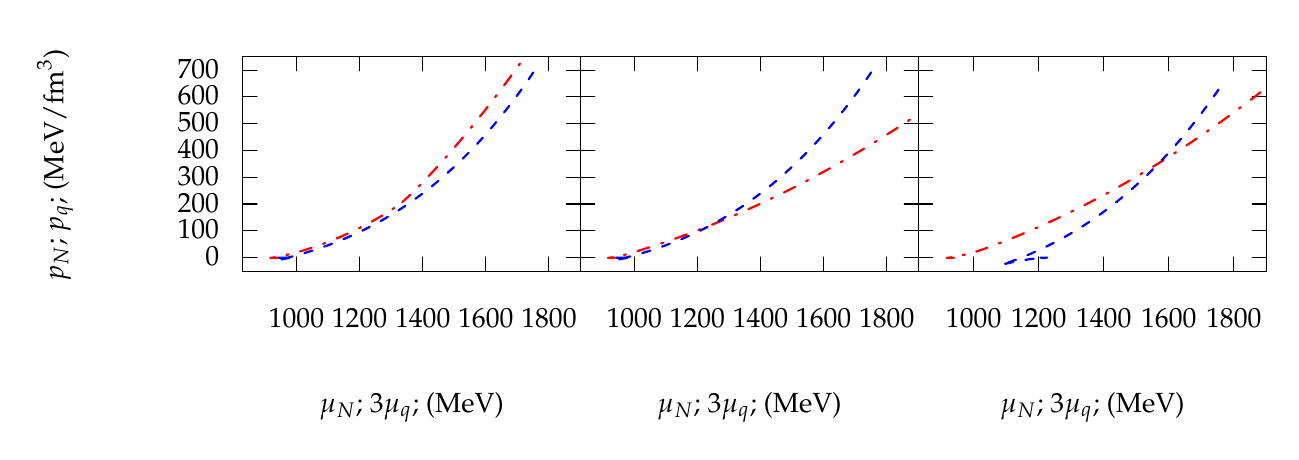
\begin{tikzpicture}[gnuplot]
%% generated with GNUPLOT 5.0p4 (Lua 5.2; terminal rev. 99, script rev. 100)
%% Mon Nov 28 17:06:57 2016
\path (0.000,0.000) rectangle (13.000,5.000);
\gpcolor{color=gp lt color border}
\gpsetlinetype{gp lt border}
\gpsetdashtype{gp dt solid}
\gpsetlinewidth{1.00}
\draw[gp path] (0.000,2.079)--(0.180,2.079);
\draw[gp path] (4.289,2.079)--(4.109,2.079);
\node[gp node right] at (-0.184,2.079) {$0$};
\draw[gp path] (0.000,2.419)--(0.180,2.419);
\draw[gp path] (4.289,2.419)--(4.109,2.419);
\node[gp node right] at (-0.184,2.419) {$100$};
\draw[gp path] (0.000,2.760)--(0.180,2.760);
\draw[gp path] (4.289,2.760)--(4.109,2.760);
\node[gp node right] at (-0.184,2.760) {$200$};
\draw[gp path] (0.000,3.100)--(0.180,3.100);
\draw[gp path] (4.289,3.100)--(4.109,3.100);
\node[gp node right] at (-0.184,3.100) {$300$};
\draw[gp path] (0.000,3.440)--(0.180,3.440);
\draw[gp path] (4.289,3.440)--(4.109,3.440);
\node[gp node right] at (-0.184,3.440) {$400$};
\draw[gp path] (0.000,3.780)--(0.180,3.780);
\draw[gp path] (4.289,3.780)--(4.109,3.780);
\node[gp node right] at (-0.184,3.780) {$500$};
\draw[gp path] (0.000,4.121)--(0.180,4.121);
\draw[gp path] (4.289,4.121)--(4.109,4.121);
\node[gp node right] at (-0.184,4.121) {$600$};
\draw[gp path] (0.000,4.461)--(0.180,4.461);
\draw[gp path] (4.289,4.461)--(4.109,4.461);
\node[gp node right] at (-0.184,4.461) {$700$};
\draw[gp path] (0.681,1.909)--(0.681,2.089);
\draw[gp path] (0.681,4.631)--(0.681,4.451);
\node[gp node center] at (0.681,1.293) {$1000$};
\draw[gp path] (1.483,1.909)--(1.483,2.089);
\draw[gp path] (1.483,4.631)--(1.483,4.451);
\node[gp node center] at (1.483,1.293) {$1200$};
\draw[gp path] (2.285,1.909)--(2.285,2.089);
\draw[gp path] (2.285,4.631)--(2.285,4.451);
\node[gp node center] at (2.285,1.293) {$1400$};
\draw[gp path] (3.086,1.909)--(3.086,2.089);
\draw[gp path] (3.086,4.631)--(3.086,4.451);
\node[gp node center] at (3.086,1.293) {$1600$};
\draw[gp path] (3.888,1.909)--(3.888,2.089);
\draw[gp path] (3.888,4.631)--(3.888,4.451);
\node[gp node center] at (3.888,1.293) {$1800$};
\draw[gp path] (0.000,4.631)--(0.000,1.909)--(4.289,1.909)--(4.289,4.631)--cycle;
\node[gp node center,rotate=-270] at (-2.362,3.270) {$p_N$; $p_q$; ($\rm{MeV}/\rm{fm}^3$)};
\node[gp node center] at (2.144,0.215) {$\mu_N$; $3\mu_q$; (MeV)};
\gpcolor{rgb color={1.000,0.000,0.000}}
\gpsetdashtype{gp dt 6}
\gpsetlinewidth{2.00}
\draw[gp path] (0.439,2.079)--(0.438,2.079)--(0.437,2.079)--(0.436,2.079)--(0.435,2.079)%
  --(0.434,2.079)--(0.433,2.079)--(0.432,2.079)--(0.431,2.079)--(0.430,2.079)--(0.429,2.079)%
  --(0.428,2.079)--(0.427,2.079)--(0.426,2.079)--(0.425,2.079)--(0.424,2.079)--(0.423,2.079)%
  --(0.422,2.079)--(0.421,2.079)--(0.420,2.079)--(0.419,2.079)--(0.418,2.079)--(0.417,2.079)%
  --(0.416,2.079)--(0.415,2.079)--(0.414,2.079)--(0.413,2.079)--(0.412,2.079)--(0.411,2.079)%
  --(0.410,2.079)--(0.409,2.079)--(0.408,2.079)--(0.407,2.079)--(0.406,2.079)--(0.405,2.079)%
  --(0.404,2.079)--(0.403,2.079)--(0.402,2.079)--(0.401,2.079)--(0.400,2.079)--(0.399,2.079)%
  --(0.398,2.079)--(0.397,2.079)--(0.396,2.078)--(0.395,2.078)--(0.394,2.078)--(0.393,2.078)%
  --(0.392,2.078)--(0.391,2.078)--(0.390,2.078)--(0.389,2.078)--(0.388,2.078)--(0.387,2.078)%
  --(0.386,2.078)--(0.385,2.078)--(0.384,2.078)--(0.383,2.078)--(0.382,2.078)--(0.381,2.078)%
  --(0.380,2.078)--(0.379,2.078)--(0.378,2.078)--(0.377,2.078)--(0.376,2.078)--(0.375,2.078)%
  --(0.374,2.078)--(0.373,2.078)--(0.372,2.078)--(0.371,2.078)--(0.370,2.078)--(0.370,2.077)%
  --(0.369,2.077)--(0.368,2.077)--(0.367,2.077)--(0.366,2.077)--(0.365,2.077)--(0.364,2.077)%
  --(0.363,2.077)--(0.362,2.077)--(0.361,2.077)--(0.360,2.077)--(0.359,2.077)--(0.358,2.077)%
  --(0.357,2.077)--(0.356,2.077)--(0.355,2.077)--(0.354,2.077)--(0.353,2.077)--(0.352,2.077)%
  --(0.352,2.076)--(0.351,2.076)--(0.350,2.076)--(0.349,2.076)--(0.348,2.076)--(0.347,2.076)%
  --(0.348,2.076)--(0.349,2.076)--(0.350,2.076)--(0.351,2.076)--(0.351,2.077)--(0.352,2.077)%
  --(0.353,2.077)--(0.354,2.077)--(0.355,2.077)--(0.356,2.077)--(0.357,2.077)--(0.358,2.077)%
  --(0.359,2.077)--(0.360,2.077)--(0.360,2.078)--(0.361,2.078)--(0.362,2.078)--(0.363,2.078)%
  --(0.364,2.078)--(0.365,2.078)--(0.366,2.078)--(0.367,2.078)--(0.368,2.079)--(0.369,2.079)%
  --(0.370,2.079)--(0.371,2.079)--(0.372,2.079)--(0.373,2.079)--(0.374,2.079)--(0.375,2.080)%
  --(0.376,2.080)--(0.377,2.080)--(0.378,2.080)--(0.379,2.080)--(0.380,2.080)--(0.381,2.080)%
  --(0.382,2.080)--(0.382,2.081)--(0.383,2.081)--(0.384,2.081)--(0.385,2.081)--(0.386,2.081)%
  --(0.387,2.081)--(0.388,2.081)--(0.389,2.082)--(0.390,2.082)--(0.391,2.082)--(0.392,2.082)%
  --(0.393,2.082)--(0.394,2.082)--(0.395,2.082)--(0.396,2.083)--(0.397,2.083)--(0.398,2.083)%
  --(0.399,2.083)--(0.400,2.083)--(0.401,2.083)--(0.402,2.084)--(0.403,2.084)--(0.404,2.084)%
  --(0.405,2.084)--(0.406,2.084)--(0.407,2.084)--(0.408,2.085)--(0.409,2.085)--(0.410,2.085)%
  --(0.411,2.085)--(0.412,2.085)--(0.413,2.085)--(0.414,2.086)--(0.415,2.086)--(0.416,2.086)%
  --(0.417,2.086)--(0.418,2.086)--(0.419,2.086)--(0.420,2.087)--(0.421,2.087)--(0.422,2.087)%
  --(0.423,2.087)--(0.424,2.087)--(0.425,2.087)--(0.426,2.088)--(0.427,2.088)--(0.428,2.088)%
  --(0.429,2.088)--(0.430,2.088)--(0.431,2.088)--(0.432,2.089)--(0.433,2.089)--(0.434,2.089)%
  --(0.435,2.089)--(0.437,2.089)--(0.438,2.090)--(0.439,2.090)--(0.440,2.090)--(0.441,2.090)%
  --(0.442,2.090)--(0.443,2.091)--(0.444,2.091)--(0.445,2.091)--(0.446,2.091)--(0.447,2.091)%
  --(0.449,2.092)--(0.450,2.092)--(0.451,2.092)--(0.452,2.092)--(0.453,2.092)--(0.454,2.093)%
  --(0.455,2.093)--(0.457,2.093)--(0.458,2.093)--(0.459,2.094)--(0.460,2.094)--(0.461,2.094)%
  --(0.463,2.094)--(0.464,2.094)--(0.465,2.095)--(0.466,2.095)--(0.467,2.095)--(0.469,2.095)%
  --(0.470,2.096)--(0.471,2.096)--(0.472,2.096)--(0.473,2.096)--(0.475,2.097)--(0.476,2.097)%
  --(0.477,2.097)--(0.478,2.097)--(0.480,2.098)--(0.481,2.098)--(0.482,2.098)--(0.484,2.098)%
  --(0.485,2.099)--(0.486,2.099)--(0.487,2.099)--(0.489,2.099)--(0.490,2.100)--(0.491,2.100)%
  --(0.493,2.100)--(0.494,2.101)--(0.495,2.101)--(0.497,2.101)--(0.498,2.101)--(0.499,2.102)%
  --(0.501,2.102)--(0.502,2.102)--(0.503,2.102)--(0.505,2.103)--(0.506,2.103)--(0.507,2.103)%
  --(0.509,2.104)--(0.510,2.104)--(0.511,2.104)--(0.513,2.105)--(0.514,2.105)--(0.516,2.105)%
  --(0.517,2.105)--(0.518,2.106)--(0.520,2.106)--(0.521,2.106)--(0.523,2.107)--(0.524,2.107)%
  --(0.525,2.107)--(0.527,2.108)--(0.528,2.108)--(0.530,2.108)--(0.531,2.109)--(0.533,2.109)%
  --(0.534,2.109)--(0.535,2.109)--(0.537,2.110)--(0.538,2.110)--(0.540,2.110)--(0.541,2.111)%
  --(0.543,2.111)--(0.544,2.111)--(0.546,2.112)--(0.547,2.112)--(0.549,2.112)--(0.550,2.113)%
  --(0.552,2.113)--(0.553,2.114)--(0.555,2.114)--(0.556,2.114)--(0.558,2.115)--(0.559,2.115)%
  --(0.561,2.115)--(0.562,2.116)--(0.564,2.116)--(0.565,2.116)--(0.567,2.117)--(0.568,2.117)%
  --(0.570,2.117)--(0.572,2.118)--(0.573,2.118)--(0.575,2.119)--(0.576,2.119)--(0.578,2.119)%
  --(0.579,2.120)--(0.581,2.120)--(0.583,2.120)--(0.584,2.121)--(0.586,2.121)--(0.587,2.122)%
  --(0.589,2.122)--(0.590,2.122)--(0.592,2.123)--(0.594,2.123)--(0.595,2.124)--(0.597,2.124)%
  --(0.599,2.124)--(0.600,2.125)--(0.602,2.125)--(0.603,2.126)--(0.605,2.126)--(0.607,2.126)%
  --(0.608,2.127)--(0.610,2.127)--(0.612,2.128)--(0.613,2.128)--(0.615,2.128)--(0.617,2.129)%
  --(0.618,2.129)--(0.620,2.130)--(0.622,2.130)--(0.623,2.131)--(0.625,2.131)--(0.627,2.131)%
  --(0.628,2.132)--(0.630,2.132)--(0.632,2.133)--(0.633,2.133)--(0.635,2.134)--(0.637,2.134)%
  --(0.638,2.134)--(0.640,2.135)--(0.642,2.135)--(0.644,2.136)--(0.645,2.136)--(0.647,2.137)%
  --(0.649,2.137)--(0.650,2.138)--(0.652,2.138)--(0.654,2.139)--(0.656,2.139)--(0.657,2.139)%
  --(0.659,2.140)--(0.661,2.140)--(0.663,2.141)--(0.664,2.141)--(0.666,2.142)--(0.668,2.142)%
  --(0.670,2.143)--(0.671,2.143)--(0.673,2.144)--(0.675,2.144)--(0.677,2.145)--(0.678,2.145)%
  --(0.680,2.146)--(0.682,2.146)--(0.684,2.147)--(0.686,2.147)--(0.687,2.148)--(0.689,2.148)%
  --(0.691,2.149)--(0.693,2.149)--(0.695,2.150)--(0.696,2.150)--(0.698,2.151)--(0.700,2.151)%
  --(0.702,2.152)--(0.704,2.152)--(0.705,2.153)--(0.707,2.153)--(0.709,2.154)--(0.711,2.154)%
  --(0.713,2.155)--(0.715,2.155)--(0.716,2.156)--(0.718,2.156)--(0.720,2.157)--(0.722,2.157)%
  --(0.724,2.158)--(0.726,2.158)--(0.728,2.159)--(0.729,2.160)--(0.731,2.160)--(0.733,2.161)%
  --(0.735,2.161)--(0.737,2.162)--(0.739,2.162)--(0.741,2.163)--(0.742,2.163)--(0.744,2.164)%
  --(0.746,2.164)--(0.748,2.165)--(0.750,2.166)--(0.752,2.166)--(0.754,2.167)--(0.756,2.167)%
  --(0.758,2.168)--(0.759,2.168)--(0.761,2.169)--(0.763,2.169)--(0.765,2.170)--(0.767,2.171)%
  --(0.769,2.171)--(0.771,2.172)--(0.773,2.172)--(0.775,2.173)--(0.777,2.174)--(0.779,2.174)%
  --(0.780,2.175)--(0.782,2.175)--(0.784,2.176)--(0.786,2.176)--(0.788,2.177)--(0.790,2.178)%
  --(0.792,2.178)--(0.794,2.179)--(0.796,2.179)--(0.798,2.180)--(0.800,2.181)--(0.802,2.181)%
  --(0.804,2.182)--(0.806,2.182)--(0.808,2.183)--(0.810,2.184)--(0.812,2.184)--(0.813,2.185)%
  --(0.815,2.186)--(0.817,2.186)--(0.819,2.187)--(0.821,2.187)--(0.823,2.188)--(0.825,2.189)%
  --(0.827,2.189)--(0.829,2.190)--(0.831,2.191)--(0.833,2.191)--(0.835,2.192)--(0.837,2.192)%
  --(0.839,2.193)--(0.841,2.194)--(0.843,2.194)--(0.845,2.195)--(0.847,2.196)--(0.849,2.196)%
  --(0.851,2.197)--(0.853,2.198)--(0.855,2.198)--(0.857,2.199)--(0.859,2.200)--(0.861,2.200)%
  --(0.863,2.201)--(0.865,2.201)--(0.867,2.202)--(0.869,2.203)--(0.871,2.203)--(0.873,2.204)%
  --(0.875,2.205)--(0.877,2.205)--(0.879,2.206)--(0.881,2.207)--(0.883,2.208)--(0.885,2.208)%
  --(0.887,2.209)--(0.889,2.210)--(0.891,2.210)--(0.893,2.211)--(0.895,2.212)--(0.897,2.212)%
  --(0.899,2.213)--(0.901,2.214)--(0.903,2.214)--(0.906,2.215)--(0.908,2.216)--(0.910,2.216)%
  --(0.912,2.217)--(0.914,2.218)--(0.916,2.219)--(0.918,2.219)--(0.920,2.220)--(0.922,2.221)%
  --(0.924,2.221)--(0.926,2.222)--(0.928,2.223)--(0.930,2.223)--(0.932,2.224)--(0.934,2.225)%
  --(0.936,2.226)--(0.938,2.226)--(0.940,2.227)--(0.942,2.228)--(0.944,2.229)--(0.947,2.229)%
  --(0.949,2.230)--(0.951,2.231)--(0.953,2.231)--(0.955,2.232)--(0.957,2.233)--(0.959,2.234)%
  --(0.961,2.234)--(0.963,2.235)--(0.965,2.236)--(0.967,2.237)--(0.969,2.237)--(0.971,2.238)%
  --(0.973,2.239)--(0.976,2.240)--(0.978,2.240)--(0.980,2.241)--(0.982,2.242)--(0.984,2.243)%
  --(0.986,2.243)--(0.988,2.244)--(0.990,2.245)--(0.992,2.246)--(0.994,2.246)--(0.996,2.247)%
  --(0.998,2.248)--(1.001,2.249)--(1.003,2.249)--(1.005,2.250)--(1.007,2.251)--(1.009,2.252)%
  --(1.011,2.252)--(1.013,2.253)--(1.015,2.254)--(1.017,2.255)--(1.019,2.256)--(1.021,2.256)%
  --(1.024,2.257)--(1.026,2.258)--(1.028,2.259)--(1.030,2.259)--(1.032,2.260)--(1.034,2.261)%
  --(1.036,2.262)--(1.038,2.263)--(1.040,2.263)--(1.042,2.264)--(1.044,2.265)--(1.047,2.266)%
  --(1.049,2.267)--(1.051,2.267)--(1.053,2.268)--(1.055,2.269)--(1.057,2.270)--(1.059,2.271)%
  --(1.061,2.271)--(1.063,2.272)--(1.065,2.273)--(1.068,2.274)--(1.070,2.275)--(1.072,2.275)%
  --(1.074,2.276)--(1.076,2.277)--(1.078,2.278)--(1.080,2.279)--(1.082,2.279)--(1.084,2.280)%
  --(1.087,2.281)--(1.089,2.282)--(1.091,2.283)--(1.093,2.284)--(1.095,2.284)--(1.097,2.285)%
  --(1.099,2.286)--(1.101,2.287)--(1.103,2.288)--(1.105,2.289)--(1.108,2.289)--(1.110,2.290)%
  --(1.112,2.291)--(1.114,2.292)--(1.116,2.293)--(1.118,2.294)--(1.120,2.294)--(1.122,2.295)%
  --(1.124,2.296)--(1.127,2.297)--(1.129,2.298)--(1.131,2.299)--(1.133,2.299)--(1.135,2.300)%
  --(1.137,2.301)--(1.139,2.302)--(1.141,2.303)--(1.143,2.304)--(1.146,2.305)--(1.148,2.305)%
  --(1.150,2.306)--(1.152,2.307)--(1.154,2.308)--(1.156,2.309)--(1.158,2.310)--(1.160,2.311)%
  --(1.162,2.311)--(1.164,2.312)--(1.167,2.313)--(1.169,2.314)--(1.171,2.315)--(1.173,2.316)%
  --(1.175,2.317)--(1.177,2.317)--(1.179,2.318)--(1.181,2.319)--(1.183,2.320)--(1.185,2.321)%
  --(1.188,2.322)--(1.190,2.323)--(1.192,2.324)--(1.194,2.324)--(1.196,2.325)--(1.198,2.326)%
  --(1.200,2.327)--(1.202,2.328)--(1.204,2.329)--(1.206,2.330)--(1.209,2.331)--(1.211,2.332)%
  --(1.213,2.332)--(1.215,2.333)--(1.217,2.334)--(1.219,2.335)--(1.221,2.336)--(1.223,2.337)%
  --(1.225,2.338)--(1.227,2.339)--(1.229,2.340)--(1.232,2.340)--(1.234,2.341)--(1.236,2.342)%
  --(1.238,2.343)--(1.240,2.344)--(1.242,2.345)--(1.244,2.346)--(1.246,2.347)--(1.248,2.348)%
  --(1.250,2.349)--(1.252,2.349)--(1.254,2.350)--(1.257,2.351)--(1.259,2.352)--(1.261,2.353)%
  --(1.263,2.354)--(1.265,2.355)--(1.267,2.356)--(1.269,2.357)--(1.271,2.358)--(1.273,2.359)%
  --(1.275,2.359)--(1.277,2.360)--(1.279,2.361)--(1.281,2.362)--(1.284,2.363)--(1.286,2.364)%
  --(1.288,2.365)--(1.290,2.366)--(1.292,2.367)--(1.294,2.368)--(1.296,2.369)--(1.298,2.369)%
  --(1.300,2.370)--(1.302,2.371)--(1.304,2.372)--(1.306,2.373)--(1.308,2.374)--(1.310,2.375)%
  --(1.312,2.376)--(1.314,2.377)--(1.316,2.378)--(1.318,2.379)--(1.321,2.380)--(1.323,2.381)%
  --(1.325,2.382)--(1.327,2.382)--(1.329,2.383)--(1.331,2.384)--(1.333,2.385)--(1.335,2.386)%
  --(1.337,2.387)--(1.339,2.388)--(1.341,2.389)--(1.343,2.390)--(1.345,2.391)--(1.347,2.392)%
  --(1.349,2.393)--(1.351,2.394)--(1.353,2.395)--(1.355,2.395)--(1.357,2.396)--(1.359,2.397)%
  --(1.361,2.398)--(1.363,2.399)--(1.365,2.400)--(1.367,2.401)--(1.369,2.402)--(1.371,2.403)%
  --(1.373,2.404)--(1.375,2.405)--(1.377,2.406)--(1.379,2.407)--(1.381,2.408)--(1.383,2.409)%
  --(1.385,2.410)--(1.387,2.411)--(1.389,2.411)--(1.391,2.412)--(1.393,2.413)--(1.395,2.414)%
  --(1.397,2.415)--(1.399,2.416)--(1.401,2.417)--(1.403,2.418)--(1.405,2.419)--(1.407,2.420)%
  --(1.409,2.421)--(1.411,2.422)--(1.413,2.423)--(1.415,2.424)--(1.417,2.425)--(1.419,2.426)%
  --(1.421,2.427)--(1.423,2.428)--(1.425,2.428)--(1.427,2.429)--(1.429,2.430)--(1.431,2.431)%
  --(1.433,2.432)--(1.435,2.433)--(1.437,2.434)--(1.439,2.435)--(1.441,2.436)--(1.443,2.437)%
  --(1.444,2.438)--(1.446,2.439)--(1.448,2.440)--(1.450,2.441)--(1.452,2.442)--(1.454,2.443)%
  --(1.456,2.444)--(1.458,2.445)--(1.460,2.446)--(1.462,2.446)--(1.464,2.447)--(1.466,2.448)%
  --(1.468,2.449)--(1.470,2.450)--(1.471,2.451)--(1.473,2.452)--(1.475,2.453)--(1.477,2.454)%
  --(1.479,2.455)--(1.481,2.456)--(1.483,2.457)--(1.485,2.458)--(1.487,2.459)--(1.489,2.460)%
  --(1.491,2.461)--(1.492,2.462)--(1.494,2.463)--(1.496,2.464)--(1.498,2.465)--(1.500,2.465)%
  --(1.502,2.466)--(1.504,2.467)--(1.506,2.468)--(1.507,2.469)--(1.509,2.470)--(1.511,2.471)%
  --(1.513,2.472)--(1.515,2.473)--(1.517,2.474)--(1.519,2.475)--(1.521,2.476)--(1.522,2.477)%
  --(1.524,2.478)--(1.526,2.479)--(1.528,2.480)--(1.530,2.481)--(1.532,2.482)--(1.533,2.483)%
  --(1.535,2.483)--(1.537,2.484)--(1.539,2.485)--(1.541,2.486)--(1.543,2.487)--(1.544,2.488)%
  --(1.546,2.489)--(1.548,2.490)--(1.550,2.491)--(1.552,2.492)--(1.554,2.493)--(1.555,2.494)%
  --(1.557,2.495)--(1.559,2.496)--(1.561,2.497)--(1.563,2.498)--(1.564,2.499)--(1.566,2.500)%
  --(1.568,2.500)--(1.570,2.501)--(1.571,2.502)--(1.573,2.503)--(1.575,2.504)--(1.577,2.505)%
  --(1.579,2.506)--(1.580,2.507)--(1.582,2.508)--(1.584,2.509)--(1.586,2.510)--(1.587,2.511)%
  --(1.589,2.512)--(1.591,2.513)--(1.593,2.514)--(1.594,2.514)--(1.596,2.515)--(1.598,2.516)%
  --(1.600,2.517)--(1.601,2.518)--(1.603,2.519)--(1.605,2.520)--(1.607,2.521)--(1.608,2.522)%
  --(1.610,2.523)--(1.612,2.524)--(1.613,2.525)--(1.615,2.526)--(1.617,2.527)--(1.619,2.527)%
  --(1.620,2.528)--(1.622,2.529)--(1.624,2.530)--(1.625,2.531)--(1.627,2.532)--(1.629,2.533)%
  --(1.630,2.534)--(1.632,2.535)--(1.634,2.536)--(1.635,2.537)--(1.637,2.538)--(1.639,2.538)%
  --(1.640,2.539)--(1.642,2.540)--(1.644,2.541)--(1.645,2.542)--(1.647,2.543)--(1.649,2.544)%
  --(1.650,2.545)--(1.652,2.546)--(1.654,2.547)--(1.655,2.548)--(1.657,2.548)--(1.658,2.549)%
  --(1.660,2.550)--(1.662,2.551)--(1.663,2.552)--(1.665,2.553)--(1.667,2.554)--(1.668,2.555)%
  --(1.670,2.556)--(1.671,2.557)--(1.673,2.557)--(1.675,2.558)--(1.676,2.559)--(1.678,2.560)%
  --(1.679,2.561)--(1.681,2.562)--(1.683,2.563)--(1.684,2.564)--(1.686,2.565)--(1.687,2.565)%
  --(1.689,2.566)--(1.690,2.567)--(1.692,2.568)--(1.693,2.569)--(1.695,2.570)--(1.697,2.571)%
  --(1.698,2.572)--(1.700,2.573)--(1.701,2.573)--(1.703,2.574)--(1.704,2.575)--(1.706,2.576)%
  --(1.707,2.577)--(1.709,2.578)--(1.710,2.579)--(1.712,2.580)--(1.713,2.580)--(1.715,2.581)%
  --(1.716,2.582)--(1.718,2.583)--(1.719,2.584)--(1.721,2.585)--(1.722,2.586)--(1.724,2.586)%
  --(1.725,2.587)--(1.727,2.588)--(1.728,2.589)--(1.730,2.590)--(1.731,2.591)--(1.733,2.592)%
  --(1.734,2.592)--(1.736,2.593)--(1.737,2.594)--(1.738,2.595)--(1.740,2.596)--(1.741,2.597)%
  --(1.743,2.597)--(1.744,2.598)--(1.746,2.599)--(1.747,2.600)--(1.749,2.601)--(1.750,2.602)%
  --(1.751,2.602)--(1.753,2.603)--(1.754,2.604)--(1.756,2.605)--(1.757,2.606)--(1.758,2.607)%
  --(1.760,2.607)--(1.761,2.608)--(1.763,2.609)--(1.764,2.610)--(1.765,2.611)--(1.767,2.612)%
  --(1.768,2.612)--(1.769,2.613)--(1.771,2.614)--(1.772,2.615)--(1.773,2.616)--(1.775,2.616)%
  --(1.776,2.617)--(1.777,2.618)--(1.779,2.619)--(1.780,2.620)--(1.781,2.620)--(1.783,2.621)%
  --(1.784,2.622)--(1.785,2.623)--(1.787,2.624)--(1.788,2.624)--(1.789,2.625)--(1.791,2.626)%
  --(1.792,2.627)--(1.793,2.628)--(1.795,2.628)--(1.796,2.629)--(1.797,2.630)--(1.798,2.631)%
  --(1.800,2.631)--(1.801,2.632)--(1.802,2.633)--(1.803,2.634)--(1.805,2.635)--(1.806,2.635)%
  --(1.807,2.636)--(1.808,2.637)--(1.810,2.638)--(1.811,2.638)--(1.812,2.639)--(1.813,2.640)%
  --(1.815,2.641)--(1.816,2.641)--(1.817,2.642)--(1.818,2.643)--(1.819,2.644)--(1.821,2.644)%
  --(1.822,2.645)--(1.823,2.646)--(1.824,2.647)--(1.825,2.647)--(1.827,2.648)--(1.828,2.649)%
  --(1.829,2.650)--(1.830,2.650)--(1.831,2.651)--(1.833,2.652)--(1.834,2.653)--(1.835,2.653)%
  --(1.836,2.654)--(1.837,2.655)--(1.838,2.655)--(1.839,2.656)--(1.841,2.657)--(1.842,2.658)%
  --(1.843,2.658)--(1.844,2.659)--(1.845,2.660)--(1.846,2.660)--(1.847,2.661)--(1.848,2.662)%
  --(1.849,2.662)--(1.851,2.663)--(1.852,2.664)--(1.853,2.665)--(1.854,2.665)--(1.855,2.666)%
  --(1.856,2.667)--(1.857,2.667)--(1.858,2.668)--(1.859,2.669)--(1.860,2.669)--(1.861,2.670)%
  --(1.862,2.671)--(1.863,2.671)--(1.864,2.672)--(1.865,2.673)--(1.867,2.673)--(1.868,2.674)%
  --(1.869,2.675)--(1.870,2.675)--(1.871,2.676)--(1.872,2.677)--(1.873,2.677)--(1.874,2.678)%
  --(1.875,2.679)--(1.876,2.679)--(1.877,2.680)--(1.878,2.681)--(1.879,2.681)--(1.880,2.682)%
  --(1.881,2.682)--(1.882,2.683)--(1.882,2.684)--(1.883,2.684)--(1.884,2.685)--(1.885,2.686)%
  --(1.886,2.686)--(1.887,2.687)--(1.888,2.687)--(1.889,2.688)--(1.890,2.689)--(1.891,2.689)%
  --(1.892,2.690)--(1.893,2.690)--(1.894,2.691)--(1.895,2.692)--(1.896,2.692)--(1.896,2.693)%
  --(1.897,2.693)--(1.898,2.694)--(1.899,2.695)--(1.900,2.695)--(1.901,2.696)--(1.902,2.696)%
  --(1.903,2.697)--(1.904,2.698)--(1.905,2.699)--(1.906,2.699)--(1.907,2.700)--(1.908,2.700)%
  --(1.909,2.701)--(1.910,2.702)--(1.911,2.703)--(1.912,2.703)--(1.913,2.704)--(1.914,2.704)%
  --(1.915,2.705)--(1.916,2.706)--(1.917,2.707)--(1.918,2.707)--(1.919,2.708)--(1.920,2.709)%
  --(1.921,2.709)--(1.922,2.710)--(1.923,2.711)--(1.924,2.711)--(1.925,2.712)--(1.926,2.713)%
  --(1.927,2.713)--(1.928,2.714)--(1.929,2.715)--(1.930,2.715)--(1.931,2.716)--(1.932,2.717)%
  --(1.933,2.717)--(1.934,2.718)--(1.935,2.719)--(1.936,2.719)--(1.936,2.720)--(1.937,2.720)%
  --(1.938,2.721)--(1.939,2.722)--(1.940,2.722)--(1.940,2.723)--(1.941,2.723)--(1.942,2.724)%
  --(1.943,2.724)--(1.944,2.725)--(1.945,2.726)--(1.946,2.726)--(1.946,2.727)--(1.947,2.727)%
  --(1.948,2.728)--(1.949,2.728)--(1.949,2.729)--(1.950,2.729)--(1.951,2.730)--(1.952,2.731)%
  --(1.953,2.731)--(1.954,2.732)--(1.955,2.733)--(1.956,2.733)--(1.957,2.734)--(1.958,2.735)%
  --(1.959,2.735)--(1.959,2.736)--(1.960,2.736)--(1.960,2.737)--(1.961,2.737)--(1.962,2.737)%
  --(1.962,2.738)--(1.963,2.738)--(1.964,2.739)--(1.965,2.740)--(1.966,2.740)--(1.966,2.741)%
  --(1.967,2.741)--(1.968,2.742)--(1.969,2.742)--(1.969,2.743)--(1.970,2.743)--(1.971,2.744)%
  --(1.971,2.745)--(1.972,2.745)--(1.973,2.746)--(1.974,2.746)--(1.975,2.747)--(1.976,2.747)%
  --(1.976,2.748)--(1.977,2.748)--(1.977,2.749)--(1.978,2.749)--(1.978,2.750)--(1.979,2.750)%
  --(1.980,2.750)--(1.980,2.751)--(1.981,2.751)--(1.981,2.752)--(1.982,2.752)--(1.983,2.753)%
  --(1.984,2.753)--(1.984,2.754)--(1.985,2.754)--(1.985,2.755)--(1.986,2.755)--(1.987,2.756)%
  --(1.988,2.756)--(1.988,2.757)--(1.989,2.757)--(1.989,2.758)--(1.990,2.758)--(1.991,2.759)%
  --(1.992,2.759)--(1.992,2.760)--(1.993,2.760)--(1.993,2.761)--(1.994,2.761)--(1.995,2.762)%
  --(1.996,2.762)--(1.996,2.763)--(1.997,2.763)--(1.997,2.764)--(1.998,2.764)--(1.999,2.765)%
  --(2.000,2.765)--(2.000,2.766)--(2.001,2.766)--(2.001,2.767)--(2.002,2.767)--(2.002,2.768)%
  --(2.003,2.768)--(2.004,2.769)--(2.005,2.769)--(2.005,2.770)--(2.006,2.770)--(2.006,2.771)%
  --(2.007,2.771)--(2.007,2.772)--(2.008,2.772)--(2.009,2.772)--(2.009,2.773)--(2.010,2.773)%
  --(2.010,2.774)--(2.011,2.774)--(2.011,2.775)--(2.012,2.775)--(2.012,2.776)--(2.013,2.776)%
  --(2.014,2.776)--(2.014,2.777)--(2.015,2.777)--(2.015,2.778)--(2.016,2.778)--(2.016,2.779)%
  --(2.017,2.779)--(2.017,2.780)--(2.018,2.780)--(2.019,2.781)--(2.020,2.781)--(2.020,2.782)%
  --(2.021,2.782)--(2.021,2.783)--(2.022,2.783)--(2.022,2.784)--(2.023,2.784)--(2.023,2.785)%
  --(2.024,2.785)--(2.024,2.786)--(2.025,2.786)--(2.026,2.786)--(2.026,2.787)--(2.027,2.787)%
  --(2.027,2.788)--(2.028,2.788)--(2.028,2.789)--(2.029,2.789)--(2.029,2.790)--(2.030,2.790)%
  --(2.030,2.791)--(2.031,2.791)--(2.032,2.792)--(2.033,2.793)--(2.034,2.793)--(2.034,2.794)%
  --(2.035,2.794)--(2.035,2.795)--(2.036,2.795)--(2.036,2.796)--(2.037,2.796)--(2.038,2.797)%
  --(2.039,2.798)--(2.040,2.799)--(2.041,2.800)--(2.042,2.801)--(2.043,2.801)--(2.043,2.802)%
  --(2.044,2.802)--(2.044,2.803)--(2.045,2.803)--(2.045,2.804)--(2.046,2.804)--(2.047,2.805)%
  --(2.048,2.806)--(2.049,2.807)--(2.050,2.807)--(2.050,2.808)--(2.051,2.808)--(2.051,2.809)%
  --(2.052,2.809)--(2.052,2.810)--(2.053,2.810)--(2.053,2.811)--(2.054,2.811)--(2.054,2.812)%
  --(2.055,2.812)--(2.056,2.813)--(2.057,2.814)--(2.058,2.815)--(2.059,2.816)--(2.060,2.817)%
  --(2.061,2.818)--(2.062,2.818)--(2.063,2.819)--(2.064,2.820)--(2.065,2.821)--(2.066,2.822)%
  --(2.066,2.823)--(2.067,2.823)--(2.068,2.824)--(2.069,2.825)--(2.070,2.826)--(2.071,2.826)%
  --(2.071,2.827)--(2.072,2.827)--(2.072,2.828)--(2.073,2.828)--(2.074,2.829)--(2.074,2.830)%
  --(2.075,2.830)--(2.075,2.831)--(2.076,2.831)--(2.077,2.832)--(2.077,2.833)--(2.078,2.833)%
  --(2.079,2.834)--(2.080,2.835)--(2.081,2.836)--(2.082,2.837)--(2.083,2.837)--(2.083,2.838)%
  --(2.084,2.839)--(2.085,2.839)--(2.085,2.840)--(2.086,2.841)--(2.087,2.841)--(2.088,2.842)%
  --(2.088,2.843)--(2.089,2.843)--(2.090,2.844)--(2.090,2.845)--(2.091,2.845)--(2.092,2.846)%
  --(2.093,2.847)--(2.094,2.848)--(2.095,2.849)--(2.096,2.849)--(2.096,2.850)--(2.097,2.851)%
  --(2.098,2.852)--(2.099,2.852)--(2.099,2.853)--(2.100,2.854)--(2.101,2.854)--(2.102,2.855)%
  --(2.103,2.856)--(2.103,2.857)--(2.104,2.857)--(2.105,2.858)--(2.106,2.859)--(2.107,2.860)%
  --(2.108,2.861)--(2.109,2.862)--(2.110,2.863)--(2.111,2.864)--(2.112,2.864)--(2.112,2.865)%
  --(2.113,2.866)--(2.114,2.867)--(2.115,2.868)--(2.116,2.868)--(2.117,2.869)--(2.118,2.870)%
  --(2.118,2.871)--(2.119,2.872)--(2.120,2.873)--(2.121,2.873)--(2.122,2.874)--(2.123,2.875)%
  --(2.124,2.876)--(2.125,2.877)--(2.126,2.878)--(2.127,2.879)--(2.128,2.880)--(2.129,2.881)%
  --(2.130,2.882)--(2.131,2.883)--(2.132,2.884)--(2.133,2.885)--(2.134,2.886)--(2.135,2.887)%
  --(2.136,2.888)--(2.137,2.888)--(2.138,2.889)--(2.139,2.890)--(2.140,2.891)--(2.141,2.892)%
  --(2.142,2.893)--(2.143,2.894)--(2.144,2.895)--(2.145,2.896)--(2.146,2.897)--(2.147,2.898)%
  --(2.148,2.899)--(2.149,2.900)--(2.150,2.901)--(2.151,2.902)--(2.152,2.903)--(2.153,2.904)%
  --(2.154,2.905)--(2.155,2.906)--(2.156,2.907)--(2.157,2.908)--(2.158,2.909)--(2.159,2.910)%
  --(2.160,2.911)--(2.161,2.912)--(2.162,2.913)--(2.163,2.914)--(2.164,2.915)--(2.165,2.916)%
  --(2.167,2.917)--(2.168,2.918)--(2.169,2.919)--(2.170,2.920)--(2.171,2.921)--(2.172,2.923)%
  --(2.173,2.924)--(2.174,2.925)--(2.175,2.926)--(2.176,2.927)--(2.178,2.928)--(2.179,2.929)%
  --(2.180,2.930)--(2.181,2.931)--(2.182,2.932)--(2.183,2.934)--(2.184,2.935)--(2.185,2.936)%
  --(2.187,2.937)--(2.188,2.938)--(2.189,2.939)--(2.190,2.940)--(2.191,2.942)--(2.192,2.943)%
  --(2.194,2.944)--(2.195,2.945)--(2.196,2.946)--(2.197,2.947)--(2.198,2.949)--(2.200,2.950)%
  --(2.201,2.951)--(2.202,2.952)--(2.203,2.953)--(2.204,2.955)--(2.206,2.956)--(2.207,2.957)%
  --(2.208,2.958)--(2.209,2.959)--(2.210,2.961)--(2.212,2.962)--(2.213,2.963)--(2.214,2.964)%
  --(2.215,2.966)--(2.217,2.967)--(2.218,2.968)--(2.219,2.969)--(2.220,2.971)--(2.222,2.972)%
  --(2.223,2.973)--(2.224,2.974)--(2.226,2.976)--(2.227,2.977)--(2.228,2.978)--(2.229,2.980)%
  --(2.231,2.981)--(2.232,2.982)--(2.233,2.983)--(2.235,2.985)--(2.236,2.986)--(2.237,2.987)%
  --(2.238,2.989)--(2.240,2.990)--(2.241,2.991)--(2.242,2.993)--(2.244,2.994)--(2.245,2.995)%
  --(2.246,2.997)--(2.248,2.998)--(2.249,2.999)--(2.250,3.001)--(2.252,3.002)--(2.253,3.004)%
  --(2.254,3.005)--(2.256,3.006)--(2.257,3.008)--(2.258,3.009)--(2.260,3.010)--(2.261,3.012)%
  --(2.263,3.013)--(2.264,3.015)--(2.265,3.016)--(2.267,3.018)--(2.268,3.019)--(2.269,3.020)%
  --(2.271,3.022)--(2.272,3.023)--(2.274,3.025)--(2.275,3.026)--(2.276,3.028)--(2.278,3.029)%
  --(2.279,3.030)--(2.281,3.032)--(2.282,3.033)--(2.284,3.035)--(2.285,3.036)--(2.286,3.038)%
  --(2.288,3.039)--(2.289,3.041)--(2.291,3.042)--(2.292,3.044)--(2.294,3.045)--(2.295,3.047)%
  --(2.296,3.048)--(2.298,3.050)--(2.299,3.051)--(2.301,3.053)--(2.302,3.054)--(2.304,3.056)%
  --(2.305,3.057)--(2.307,3.059)--(2.308,3.060)--(2.310,3.062)--(2.311,3.063)--(2.313,3.065)%
  --(2.314,3.066)--(2.316,3.068)--(2.317,3.069)--(2.319,3.071)--(2.320,3.073)--(2.322,3.074)%
  --(2.323,3.076)--(2.325,3.077)--(2.326,3.079)--(2.328,3.080)--(2.329,3.082)--(2.331,3.084)%
  --(2.332,3.085)--(2.334,3.087)--(2.335,3.088)--(2.337,3.090)--(2.338,3.092)--(2.340,3.093)%
  --(2.341,3.095)--(2.343,3.097)--(2.344,3.098)--(2.346,3.100)--(2.347,3.101)--(2.349,3.103)%
  --(2.351,3.105)--(2.352,3.106)--(2.354,3.108)--(2.355,3.110)--(2.357,3.111)--(2.358,3.113)%
  --(2.360,3.115)--(2.362,3.116)--(2.363,3.118)--(2.365,3.120)--(2.366,3.121)--(2.368,3.123)%
  --(2.369,3.125)--(2.371,3.126)--(2.373,3.128)--(2.374,3.130)--(2.376,3.131)--(2.377,3.133)%
  --(2.379,3.135)--(2.381,3.136)--(2.382,3.138)--(2.384,3.140)--(2.385,3.142)--(2.387,3.143)%
  --(2.389,3.145)--(2.390,3.147)--(2.392,3.149)--(2.394,3.150)--(2.395,3.152)--(2.397,3.154)%
  --(2.398,3.156)--(2.400,3.157)--(2.402,3.159)--(2.403,3.161)--(2.405,3.163)--(2.407,3.164)%
  --(2.408,3.166)--(2.410,3.168)--(2.412,3.170)--(2.413,3.171)--(2.415,3.173)--(2.417,3.175)%
  --(2.418,3.177)--(2.420,3.179)--(2.422,3.180)--(2.423,3.182)--(2.425,3.184)--(2.427,3.186)%
  --(2.428,3.188)--(2.430,3.189)--(2.432,3.191)--(2.433,3.193)--(2.435,3.195)--(2.437,3.197)%
  --(2.438,3.199)--(2.440,3.200)--(2.442,3.202)--(2.443,3.204)--(2.445,3.206)--(2.447,3.208)%
  --(2.448,3.210)--(2.450,3.211)--(2.452,3.213)--(2.454,3.215)--(2.455,3.217)--(2.457,3.219)%
  --(2.459,3.221)--(2.460,3.223)--(2.462,3.225)--(2.464,3.226)--(2.466,3.228)--(2.467,3.230)%
  --(2.469,3.232)--(2.471,3.234)--(2.473,3.236)--(2.474,3.238)--(2.476,3.240)--(2.478,3.242)%
  --(2.479,3.243)--(2.481,3.245)--(2.483,3.247)--(2.485,3.249)--(2.486,3.251)--(2.488,3.253)%
  --(2.490,3.255)--(2.492,3.257)--(2.493,3.259)--(2.495,3.261)--(2.497,3.263)--(2.499,3.265)%
  --(2.500,3.267)--(2.502,3.269)--(2.504,3.271)--(2.506,3.273)--(2.508,3.275)--(2.509,3.276)%
  --(2.511,3.278)--(2.513,3.280)--(2.515,3.282)--(2.516,3.284)--(2.518,3.286)--(2.520,3.288)%
  --(2.522,3.290)--(2.524,3.292)--(2.525,3.294)--(2.527,3.296)--(2.529,3.298)--(2.531,3.300)%
  --(2.533,3.302)--(2.534,3.304)--(2.536,3.306)--(2.538,3.308)--(2.540,3.310)--(2.542,3.312)%
  --(2.543,3.314)--(2.545,3.316)--(2.547,3.318)--(2.549,3.320)--(2.551,3.323)--(2.552,3.325)%
  --(2.554,3.327)--(2.556,3.329)--(2.558,3.331)--(2.560,3.333)--(2.562,3.335)--(2.563,3.337)%
  --(2.565,3.339)--(2.567,3.341)--(2.569,3.343)--(2.571,3.345)--(2.573,3.347)--(2.574,3.349)%
  --(2.576,3.351)--(2.578,3.353)--(2.580,3.355)--(2.582,3.358)--(2.584,3.360)--(2.585,3.362)%
  --(2.587,3.364)--(2.589,3.366)--(2.591,3.368)--(2.593,3.370)--(2.595,3.372)--(2.597,3.374)%
  --(2.598,3.376)--(2.600,3.379)--(2.602,3.381)--(2.604,3.383)--(2.606,3.385)--(2.608,3.387)%
  --(2.610,3.389)--(2.611,3.391)--(2.613,3.393)--(2.615,3.396)--(2.617,3.398)--(2.619,3.400)%
  --(2.621,3.402)--(2.623,3.404)--(2.625,3.406)--(2.626,3.408)--(2.628,3.411)--(2.630,3.413)%
  --(2.632,3.415)--(2.634,3.417)--(2.636,3.419)--(2.638,3.421)--(2.640,3.424)--(2.641,3.426)%
  --(2.643,3.428)--(2.645,3.430)--(2.647,3.432)--(2.649,3.434)--(2.651,3.437)--(2.653,3.439)%
  --(2.655,3.441)--(2.657,3.443)--(2.659,3.445)--(2.660,3.448)--(2.662,3.450)--(2.664,3.452)%
  --(2.666,3.454)--(2.668,3.456)--(2.670,3.459)--(2.672,3.461)--(2.674,3.463)--(2.676,3.465)%
  --(2.678,3.468)--(2.680,3.470)--(2.682,3.472)--(2.683,3.474)--(2.685,3.476)--(2.687,3.479)%
  --(2.689,3.481)--(2.691,3.483)--(2.693,3.485)--(2.695,3.488)--(2.697,3.490)--(2.699,3.492)%
  --(2.701,3.494)--(2.703,3.497)--(2.705,3.499)--(2.707,3.501)--(2.709,3.503)--(2.710,3.506)%
  --(2.712,3.508)--(2.714,3.510)--(2.716,3.513)--(2.718,3.515)--(2.720,3.517)--(2.722,3.519)%
  --(2.724,3.522)--(2.726,3.524)--(2.728,3.526)--(2.730,3.528)--(2.732,3.531)--(2.734,3.533)%
  --(2.736,3.535)--(2.738,3.538)--(2.740,3.540)--(2.742,3.542)--(2.744,3.545)--(2.746,3.547)%
  --(2.748,3.549)--(2.749,3.552)--(2.751,3.554)--(2.753,3.556)--(2.755,3.559)--(2.757,3.561)%
  --(2.759,3.563)--(2.761,3.565)--(2.763,3.568)--(2.765,3.570)--(2.767,3.572)--(2.769,3.575)%
  --(2.771,3.577)--(2.773,3.580)--(2.775,3.582)--(2.777,3.584)--(2.779,3.587)--(2.781,3.589)%
  --(2.783,3.591)--(2.785,3.594)--(2.787,3.596)--(2.789,3.598)--(2.791,3.601)--(2.793,3.603)%
  --(2.795,3.605)--(2.797,3.608)--(2.799,3.610)--(2.801,3.613)--(2.803,3.615)--(2.805,3.617)%
  --(2.807,3.620)--(2.809,3.622)--(2.811,3.625)--(2.813,3.627)--(2.815,3.629)--(2.817,3.632)%
  --(2.819,3.634)--(2.821,3.636)--(2.823,3.639)--(2.825,3.641)--(2.827,3.644)--(2.829,3.646)%
  --(2.831,3.649)--(2.833,3.651)--(2.835,3.653)--(2.837,3.656)--(2.839,3.658)--(2.841,3.661)%
  --(2.843,3.663)--(2.845,3.665)--(2.847,3.668)--(2.849,3.670)--(2.851,3.673)--(2.853,3.675)%
  --(2.855,3.678)--(2.857,3.680)--(2.859,3.683)--(2.861,3.685)--(2.863,3.687)--(2.865,3.690)%
  --(2.867,3.692)--(2.869,3.695)--(2.871,3.697)--(2.873,3.700)--(2.875,3.702)--(2.877,3.705)%
  --(2.879,3.707)--(2.881,3.710)--(2.883,3.712)--(2.885,3.714)--(2.887,3.717)--(2.889,3.719)%
  --(2.891,3.722)--(2.893,3.724)--(2.895,3.727)--(2.897,3.729)--(2.899,3.732)--(2.901,3.734)%
  --(2.903,3.737)--(2.905,3.739)--(2.908,3.742)--(2.910,3.744)--(2.912,3.747)--(2.914,3.749)%
  --(2.916,3.752)--(2.918,3.754)--(2.920,3.757)--(2.922,3.759)--(2.924,3.762)--(2.926,3.764)%
  --(2.928,3.767)--(2.930,3.769)--(2.932,3.772)--(2.934,3.774)--(2.936,3.777)--(2.938,3.779)%
  --(2.940,3.782)--(2.942,3.784)--(2.944,3.787)--(2.946,3.790)--(2.948,3.792)--(2.950,3.795)%
  --(2.952,3.797)--(2.955,3.800)--(2.957,3.802)--(2.959,3.805)--(2.961,3.807)--(2.963,3.810)%
  --(2.965,3.812)--(2.967,3.815)--(2.969,3.818)--(2.971,3.820)--(2.973,3.823)--(2.975,3.825)%
  --(2.977,3.828)--(2.979,3.830)--(2.981,3.833)--(2.983,3.835)--(2.985,3.838)--(2.987,3.841)%
  --(2.989,3.843)--(2.992,3.846)--(2.994,3.848)--(2.996,3.851)--(2.998,3.854)--(3.000,3.856)%
  --(3.002,3.859)--(3.004,3.861)--(3.006,3.864)--(3.008,3.866)--(3.010,3.869)--(3.012,3.872)%
  --(3.014,3.874)--(3.016,3.877)--(3.018,3.879)--(3.021,3.882)--(3.023,3.885)--(3.025,3.887)%
  --(3.027,3.890)--(3.029,3.892)--(3.031,3.895)--(3.033,3.898)--(3.035,3.900)--(3.037,3.903)%
  --(3.039,3.906)--(3.041,3.908)--(3.043,3.911)--(3.045,3.913)--(3.048,3.916)--(3.050,3.919)%
  --(3.052,3.921)--(3.054,3.924)--(3.056,3.927)--(3.058,3.929)--(3.060,3.932)--(3.062,3.935)%
  --(3.064,3.937)--(3.066,3.940)--(3.068,3.942)--(3.070,3.945)--(3.073,3.948)--(3.075,3.950)%
  --(3.077,3.953)--(3.079,3.956)--(3.081,3.958)--(3.083,3.961)--(3.085,3.964)--(3.087,3.966)%
  --(3.089,3.969)--(3.091,3.972)--(3.093,3.974)--(3.096,3.977)--(3.098,3.980)--(3.100,3.982)%
  --(3.102,3.985)--(3.104,3.988)--(3.106,3.990)--(3.108,3.993)--(3.110,3.996)--(3.112,3.999)%
  --(3.114,4.001)--(3.116,4.004)--(3.119,4.007)--(3.121,4.009)--(3.123,4.012)--(3.125,4.015)%
  --(3.127,4.017)--(3.129,4.020)--(3.131,4.023)--(3.133,4.025)--(3.135,4.028)--(3.137,4.031)%
  --(3.140,4.034)--(3.142,4.036)--(3.144,4.039)--(3.146,4.042)--(3.148,4.044)--(3.150,4.047)%
  --(3.152,4.050)--(3.154,4.053)--(3.156,4.055)--(3.159,4.058)--(3.161,4.061)--(3.163,4.064)%
  --(3.165,4.066)--(3.167,4.069)--(3.169,4.072)--(3.171,4.074)--(3.173,4.077)--(3.175,4.080)%
  --(3.177,4.083)--(3.180,4.085)--(3.182,4.088)--(3.184,4.091)--(3.186,4.094)--(3.188,4.096)%
  --(3.190,4.099)--(3.192,4.102)--(3.194,4.105)--(3.197,4.107)--(3.199,4.110)--(3.201,4.113)%
  --(3.203,4.116)--(3.205,4.119)--(3.207,4.121)--(3.209,4.124)--(3.211,4.127)--(3.213,4.130)%
  --(3.216,4.132)--(3.218,4.135)--(3.220,4.138)--(3.222,4.141)--(3.224,4.143)--(3.226,4.146)%
  --(3.228,4.149)--(3.230,4.152)--(3.233,4.155)--(3.235,4.157)--(3.237,4.160)--(3.239,4.163)%
  --(3.241,4.166)--(3.243,4.169)--(3.245,4.171)--(3.247,4.174)--(3.250,4.177)--(3.252,4.180)%
  --(3.254,4.183)--(3.256,4.185)--(3.258,4.188)--(3.260,4.191)--(3.262,4.194)--(3.264,4.197)%
  --(3.267,4.199)--(3.269,4.202)--(3.271,4.205)--(3.273,4.208)--(3.275,4.211)--(3.277,4.214)%
  --(3.279,4.216)--(3.281,4.219)--(3.284,4.222)--(3.286,4.225)--(3.288,4.228)--(3.290,4.230)%
  --(3.292,4.233)--(3.294,4.236)--(3.296,4.239)--(3.298,4.242)--(3.301,4.245)--(3.303,4.248)%
  --(3.305,4.250)--(3.307,4.253)--(3.309,4.256)--(3.311,4.259)--(3.313,4.262)--(3.316,4.265)%
  --(3.318,4.267)--(3.320,4.270)--(3.322,4.273)--(3.324,4.276)--(3.326,4.279)--(3.328,4.282)%
  --(3.330,4.285)--(3.333,4.287)--(3.335,4.290)--(3.337,4.293)--(3.339,4.296)--(3.341,4.299)%
  --(3.343,4.302)--(3.345,4.305)--(3.348,4.308)--(3.350,4.310)--(3.352,4.313)--(3.354,4.316)%
  --(3.356,4.319)--(3.358,4.322)--(3.360,4.325)--(3.363,4.328)--(3.365,4.331)--(3.367,4.334)%
  --(3.369,4.336)--(3.371,4.339)--(3.373,4.342)--(3.375,4.345)--(3.378,4.348)--(3.380,4.351)%
  --(3.382,4.354)--(3.384,4.357)--(3.386,4.360)--(3.388,4.362)--(3.390,4.365)--(3.393,4.368)%
  --(3.395,4.371)--(3.397,4.374)--(3.399,4.377)--(3.401,4.380)--(3.403,4.383)--(3.405,4.386)%
  --(3.408,4.389)--(3.410,4.392)--(3.412,4.395)--(3.414,4.397)--(3.416,4.400)--(3.418,4.403)%
  --(3.420,4.406)--(3.423,4.409)--(3.425,4.412)--(3.427,4.415)--(3.429,4.418)--(3.431,4.421)%
  --(3.433,4.424)--(3.435,4.427)--(3.438,4.430)--(3.440,4.433)--(3.442,4.436)--(3.444,4.439)%
  --(3.446,4.442)--(3.448,4.444)--(3.451,4.447)--(3.453,4.450)--(3.455,4.453)--(3.457,4.456)%
  --(3.459,4.459)--(3.461,4.462)--(3.463,4.465)--(3.466,4.468)--(3.468,4.471)--(3.470,4.474)%
  --(3.472,4.477)--(3.474,4.480)--(3.476,4.483)--(3.479,4.486)--(3.481,4.489)--(3.483,4.492)%
  --(3.485,4.495)--(3.487,4.498)--(3.489,4.501)--(3.491,4.504)--(3.494,4.507)--(3.496,4.510)%
  --(3.498,4.513)--(3.500,4.516)--(3.502,4.519)--(3.504,4.522)--(3.507,4.525)--(3.509,4.528)%
  --(3.511,4.531)--(3.513,4.534)--(3.515,4.537)--(3.517,4.540)--(3.519,4.543)--(3.522,4.546)%
  --(3.524,4.549)--(3.526,4.552)--(3.528,4.555)--(3.530,4.558)--(3.532,4.561)--(3.535,4.564)%
  --(3.537,4.567)--(3.539,4.570)--(3.541,4.573)--(3.543,4.576)--(3.545,4.579)--(3.548,4.582)%
  --(3.550,4.585)--(3.552,4.588)--(3.554,4.591)--(3.556,4.594)--(3.558,4.597)--(3.561,4.600)%
  --(3.563,4.603)--(3.565,4.606)--(3.567,4.609)--(3.569,4.612)--(3.571,4.615)--(3.573,4.618)%
  --(3.576,4.621)--(3.578,4.624)--(3.580,4.627)--(3.582,4.630)--(3.583,4.631);
\gpcolor{rgb color={0.000,0.000,1.000}}
\gpsetdashtype{gp dt 3}
\draw[gp path] (0.455,2.079)--(0.485,2.079)--(0.505,2.079)--(0.522,2.079)--(0.535,2.079)%
  --(0.547,2.079)--(0.557,2.080)--(0.566,2.080)--(0.574,2.080)--(0.581,2.080)--(0.588,2.080)%
  --(0.594,2.080)--(0.599,2.080)--(0.604,2.080)--(0.609,2.080)--(0.613,2.080)--(0.617,2.081)%
  --(0.621,2.081)--(0.624,2.081)--(0.627,2.081)--(0.630,2.081)--(0.633,2.081)--(0.635,2.081)%
  --(0.638,2.081)--(0.640,2.081)--(0.642,2.081)--(0.643,2.081)--(0.645,2.081)--(0.646,2.082)%
  --(0.647,2.082)--(0.649,2.082)--(0.650,2.082)--(0.651,2.082)--(0.652,2.082)--(0.653,2.082)%
  --(0.654,2.082)--(0.653,2.082)--(0.652,2.082)--(0.651,2.082)--(0.650,2.082)--(0.649,2.082)%
  --(0.648,2.081)--(0.647,2.081)--(0.646,2.081)--(0.645,2.081)--(0.644,2.081)--(0.643,2.081)%
  --(0.642,2.081)--(0.641,2.081)--(0.640,2.081)--(0.638,2.081)--(0.637,2.080)--(0.636,2.080)%
  --(0.634,2.080)--(0.633,2.080)--(0.631,2.080)--(0.630,2.080)--(0.628,2.080)--(0.627,2.079)%
  --(0.625,2.079)--(0.624,2.079)--(0.622,2.079)--(0.620,2.079)--(0.619,2.078)--(0.617,2.078)%
  --(0.615,2.078)--(0.613,2.078)--(0.611,2.078)--(0.610,2.077)--(0.608,2.077)--(0.606,2.077)%
  --(0.604,2.077)--(0.602,2.076)--(0.600,2.076)--(0.598,2.076)--(0.596,2.076)--(0.594,2.075)%
  --(0.592,2.075)--(0.590,2.075)--(0.587,2.074)--(0.585,2.074)--(0.583,2.074)--(0.581,2.074)%
  --(0.579,2.073)--(0.576,2.073)--(0.574,2.073)--(0.572,2.072)--(0.569,2.072)--(0.567,2.072)%
  --(0.565,2.071)--(0.562,2.071)--(0.560,2.070)--(0.558,2.070)--(0.555,2.070)--(0.553,2.069)%
  --(0.550,2.069)--(0.548,2.068)--(0.545,2.068)--(0.543,2.068)--(0.540,2.067)--(0.538,2.067)%
  --(0.535,2.066)--(0.533,2.066)--(0.530,2.065)--(0.527,2.065)--(0.525,2.064)--(0.522,2.064)%
  --(0.519,2.063)--(0.517,2.063)--(0.514,2.062)--(0.511,2.062)--(0.509,2.061)--(0.506,2.061)%
  --(0.503,2.060)--(0.500,2.060)--(0.498,2.059)--(0.495,2.059)--(0.492,2.058)--(0.489,2.058)%
  --(0.486,2.057)--(0.483,2.057)--(0.481,2.056)--(0.478,2.055)--(0.475,2.055)--(0.472,2.054)%
  --(0.469,2.054)--(0.466,2.053)--(0.463,2.052)--(0.460,2.052)--(0.457,2.051)--(0.454,2.050)%
  --(0.451,2.050)--(0.448,2.049)--(0.445,2.049)--(0.442,2.048)--(0.439,2.047)--(0.436,2.047)%
  --(0.433,2.046)--(0.438,2.047)--(0.447,2.049)--(0.455,2.051)--(0.463,2.053)--(0.471,2.055)%
  --(0.479,2.056)--(0.487,2.058)--(0.495,2.060)--(0.504,2.062)--(0.511,2.064)--(0.519,2.066)%
  --(0.527,2.068)--(0.535,2.070)--(0.543,2.072)--(0.551,2.074)--(0.559,2.076)--(0.566,2.078)%
  --(0.574,2.080)--(0.582,2.082)--(0.590,2.084)--(0.597,2.086)--(0.605,2.088)--(0.612,2.090)%
  --(0.620,2.092)--(0.627,2.094)--(0.635,2.096)--(0.642,2.098)--(0.650,2.100)--(0.657,2.102)%
  --(0.665,2.104)--(0.672,2.106)--(0.679,2.108)--(0.687,2.110)--(0.694,2.112)--(0.701,2.114)%
  --(0.708,2.116)--(0.716,2.118)--(0.723,2.120)--(0.730,2.122)--(0.737,2.124)--(0.744,2.126)%
  --(0.751,2.128)--(0.758,2.130)--(0.765,2.132)--(0.772,2.134)--(0.779,2.136)--(0.786,2.138)%
  --(0.793,2.140)--(0.800,2.143)--(0.807,2.145)--(0.814,2.147)--(0.821,2.149)--(0.827,2.151)%
  --(0.834,2.153)--(0.841,2.155)--(0.848,2.157)--(0.854,2.159)--(0.861,2.161)--(0.868,2.163)%
  --(0.875,2.166)--(0.881,2.168)--(0.888,2.170)--(0.894,2.172)--(0.901,2.174)--(0.908,2.176)%
  --(0.914,2.178)--(0.921,2.181)--(0.927,2.183)--(0.934,2.185)--(0.940,2.187)--(0.946,2.189)%
  --(0.953,2.191)--(0.959,2.193)--(0.966,2.196)--(0.972,2.198)--(0.978,2.200)--(0.985,2.202)%
  --(0.991,2.204)--(0.997,2.206)--(1.004,2.209)--(1.010,2.211)--(1.016,2.213)--(1.022,2.215)%
  --(1.028,2.217)--(1.035,2.220)--(1.041,2.222)--(1.047,2.224)--(1.053,2.226)--(1.059,2.228)%
  --(1.065,2.231)--(1.071,2.233)--(1.077,2.235)--(1.083,2.237)--(1.089,2.239)--(1.095,2.242)%
  --(1.101,2.244)--(1.107,2.246)--(1.113,2.248)--(1.119,2.251)--(1.125,2.253)--(1.131,2.255)%
  --(1.137,2.257)--(1.143,2.260)--(1.149,2.262)--(1.155,2.264)--(1.161,2.266)--(1.166,2.269)%
  --(1.172,2.271)--(1.178,2.273)--(1.184,2.275)--(1.190,2.278)--(1.195,2.280)--(1.201,2.282)%
  --(1.207,2.285)--(1.212,2.287)--(1.218,2.289)--(1.224,2.291)--(1.229,2.294)--(1.235,2.296)%
  --(1.241,2.298)--(1.246,2.301)--(1.252,2.303)--(1.258,2.305)--(1.263,2.308)--(1.269,2.310)%
  --(1.274,2.312)--(1.280,2.315)--(1.285,2.317)--(1.291,2.319)--(1.296,2.321)--(1.302,2.324)%
  --(1.307,2.326)--(1.313,2.328)--(1.318,2.331)--(1.324,2.333)--(1.329,2.336)--(1.334,2.338)%
  --(1.340,2.340)--(1.345,2.343)--(1.351,2.345)--(1.356,2.347)--(1.361,2.350)--(1.367,2.352)%
  --(1.372,2.354)--(1.377,2.357)--(1.383,2.359)--(1.388,2.361)--(1.393,2.364)--(1.398,2.366)%
  --(1.404,2.369)--(1.409,2.371)--(1.414,2.373)--(1.419,2.376)--(1.425,2.378)--(1.430,2.381)%
  --(1.435,2.383)--(1.440,2.385)--(1.445,2.388)--(1.450,2.390)--(1.456,2.393)--(1.461,2.395)%
  --(1.466,2.397)--(1.471,2.400)--(1.476,2.402)--(1.481,2.405)--(1.486,2.407)--(1.491,2.410)%
  --(1.496,2.412)--(1.501,2.414)--(1.506,2.417)--(1.511,2.419)--(1.516,2.422)--(1.521,2.424)%
  --(1.526,2.427)--(1.531,2.429)--(1.536,2.431)--(1.541,2.434)--(1.546,2.436)--(1.551,2.439)%
  --(1.556,2.441)--(1.561,2.444)--(1.566,2.446)--(1.571,2.449)--(1.576,2.451)--(1.581,2.454)%
  --(1.585,2.456)--(1.590,2.459)--(1.595,2.461)--(1.600,2.464)--(1.605,2.466)--(1.610,2.469)%
  --(1.615,2.471)--(1.619,2.473)--(1.624,2.476)--(1.629,2.478)--(1.634,2.481)--(1.638,2.483)%
  --(1.643,2.486)--(1.648,2.488)--(1.653,2.491)--(1.657,2.493)--(1.662,2.496)--(1.667,2.499)%
  --(1.672,2.501)--(1.676,2.504)--(1.681,2.506)--(1.686,2.509)--(1.690,2.511)--(1.695,2.514)%
  --(1.700,2.516)--(1.704,2.519)--(1.709,2.521)--(1.713,2.524)--(1.718,2.526)--(1.723,2.529)%
  --(1.727,2.531)--(1.732,2.534)--(1.736,2.537)--(1.741,2.539)--(1.746,2.542)--(1.750,2.544)%
  --(1.755,2.547)--(1.759,2.549)--(1.764,2.552)--(1.768,2.554)--(1.773,2.557)--(1.777,2.560)%
  --(1.782,2.562)--(1.786,2.565)--(1.791,2.567)--(1.795,2.570)--(1.800,2.572)--(1.804,2.575)%
  --(1.809,2.578)--(1.813,2.580)--(1.818,2.583)--(1.822,2.585)--(1.826,2.588)--(1.831,2.591)%
  --(1.835,2.593)--(1.840,2.596)--(1.844,2.598)--(1.848,2.601)--(1.853,2.604)--(1.857,2.606)%
  --(1.862,2.609)--(1.866,2.611)--(1.870,2.614)--(1.875,2.617)--(1.879,2.619)--(1.883,2.622)%
  --(1.888,2.625)--(1.892,2.627)--(1.896,2.630)--(1.901,2.632)--(1.905,2.635)--(1.909,2.638)%
  --(1.913,2.640)--(1.918,2.643)--(1.922,2.646)--(1.926,2.648)--(1.930,2.651)--(1.935,2.654)%
  --(1.939,2.656)--(1.943,2.659)--(1.947,2.662)--(1.952,2.664)--(1.956,2.667)--(1.960,2.670)%
  --(1.964,2.672)--(1.968,2.675)--(1.973,2.678)--(1.977,2.680)--(1.981,2.683)--(1.985,2.686)%
  --(1.989,2.688)--(1.993,2.691)--(1.998,2.694)--(2.002,2.696)--(2.006,2.699)--(2.010,2.702)%
  --(2.014,2.704)--(2.018,2.707)--(2.022,2.710)--(2.026,2.712)--(2.030,2.715)--(2.035,2.718)%
  --(2.039,2.721)--(2.043,2.723)--(2.047,2.726)--(2.051,2.729)--(2.055,2.731)--(2.059,2.734)%
  --(2.063,2.737)--(2.067,2.740)--(2.071,2.742)--(2.075,2.745)--(2.079,2.748)--(2.083,2.750)%
  --(2.087,2.753)--(2.091,2.756)--(2.095,2.759)--(2.099,2.761)--(2.103,2.764)--(2.107,2.767)%
  --(2.111,2.770)--(2.115,2.772)--(2.119,2.775)--(2.123,2.778)--(2.127,2.781)--(2.131,2.783)%
  --(2.135,2.786)--(2.139,2.789)--(2.143,2.792)--(2.147,2.794)--(2.151,2.797)--(2.154,2.800)%
  --(2.158,2.803)--(2.162,2.805)--(2.166,2.808)--(2.170,2.811)--(2.174,2.814)--(2.178,2.816)%
  --(2.182,2.819)--(2.186,2.822)--(2.189,2.825)--(2.193,2.828)--(2.197,2.830)--(2.201,2.833)%
  --(2.205,2.836)--(2.209,2.839)--(2.212,2.841)--(2.216,2.844)--(2.220,2.847)--(2.224,2.850)%
  --(2.228,2.853)--(2.231,2.855)--(2.235,2.858)--(2.239,2.861)--(2.243,2.864)--(2.247,2.867)%
  --(2.250,2.869)--(2.254,2.872)--(2.258,2.875)--(2.262,2.878)--(2.265,2.881)--(2.269,2.884)%
  --(2.273,2.886)--(2.277,2.889)--(2.280,2.892)--(2.284,2.895)--(2.288,2.898)--(2.292,2.900)%
  --(2.295,2.903)--(2.299,2.906)--(2.303,2.909)--(2.306,2.912)--(2.310,2.915)--(2.314,2.918)%
  --(2.318,2.920)--(2.321,2.923)--(2.325,2.926)--(2.329,2.929)--(2.332,2.932)--(2.336,2.935)%
  --(2.340,2.937)--(2.343,2.940)--(2.347,2.943)--(2.351,2.946)--(2.354,2.949)--(2.358,2.952)%
  --(2.361,2.955)--(2.365,2.957)--(2.369,2.960)--(2.372,2.963)--(2.376,2.966)--(2.380,2.969)%
  --(2.383,2.972)--(2.387,2.975)--(2.390,2.978)--(2.394,2.980)--(2.397,2.983)--(2.401,2.986)%
  --(2.405,2.989)--(2.408,2.992)--(2.412,2.995)--(2.415,2.998)--(2.419,3.001)--(2.422,3.004)%
  --(2.426,3.007)--(2.430,3.009)--(2.433,3.012)--(2.437,3.015)--(2.440,3.018)--(2.444,3.021)%
  --(2.447,3.024)--(2.451,3.027)--(2.454,3.030)--(2.458,3.033)--(2.461,3.036)--(2.465,3.038)%
  --(2.468,3.041)--(2.472,3.044)--(2.475,3.047)--(2.479,3.050)--(2.482,3.053)--(2.486,3.056)%
  --(2.489,3.059)--(2.493,3.062)--(2.496,3.065)--(2.500,3.068)--(2.503,3.071)--(2.506,3.074)%
  --(2.510,3.077)--(2.513,3.080)--(2.517,3.082)--(2.520,3.085)--(2.524,3.088)--(2.527,3.091)%
  --(2.531,3.094)--(2.534,3.097)--(2.537,3.100)--(2.541,3.103)--(2.544,3.106)--(2.548,3.109)%
  --(2.551,3.112)--(2.554,3.115)--(2.558,3.118)--(2.561,3.121)--(2.565,3.124)--(2.568,3.127)%
  --(2.571,3.130)--(2.575,3.133)--(2.578,3.136)--(2.581,3.139)--(2.585,3.142)--(2.588,3.145)%
  --(2.591,3.148)--(2.595,3.151)--(2.598,3.154)--(2.602,3.157)--(2.605,3.160)--(2.608,3.163)%
  --(2.612,3.166)--(2.615,3.169)--(2.618,3.172)--(2.621,3.175)--(2.625,3.178)--(2.628,3.181)%
  --(2.631,3.184)--(2.635,3.187)--(2.638,3.190)--(2.641,3.193)--(2.645,3.196)--(2.648,3.199)%
  --(2.651,3.202)--(2.654,3.205)--(2.658,3.208)--(2.661,3.211)--(2.664,3.214)--(2.668,3.217)%
  --(2.671,3.220)--(2.674,3.223)--(2.677,3.226)--(2.681,3.229)--(2.684,3.232)--(2.687,3.235)%
  --(2.690,3.238)--(2.694,3.241)--(2.697,3.244)--(2.700,3.247)--(2.703,3.250)--(2.707,3.253)%
  --(2.710,3.256)--(2.713,3.259)--(2.716,3.262)--(2.719,3.265)--(2.723,3.268)--(2.726,3.271)%
  --(2.729,3.274)--(2.732,3.277)--(2.735,3.280)--(2.739,3.284)--(2.742,3.287)--(2.745,3.290)%
  --(2.748,3.293)--(2.751,3.296)--(2.755,3.299)--(2.758,3.302)--(2.761,3.305)--(2.764,3.308)%
  --(2.767,3.311)--(2.770,3.314)--(2.774,3.317)--(2.777,3.320)--(2.780,3.323)--(2.783,3.326)%
  --(2.786,3.330)--(2.789,3.333)--(2.792,3.336)--(2.796,3.339)--(2.799,3.342)--(2.802,3.345)%
  --(2.805,3.348)--(2.808,3.351)--(2.811,3.354)--(2.814,3.357)--(2.817,3.360)--(2.820,3.364)%
  --(2.824,3.367)--(2.827,3.370)--(2.830,3.373)--(2.833,3.376)--(2.836,3.379)--(2.839,3.382)%
  --(2.842,3.385)--(2.845,3.388)--(2.848,3.391)--(2.851,3.395)--(2.854,3.398)--(2.858,3.401)%
  --(2.861,3.404)--(2.864,3.407)--(2.867,3.410)--(2.870,3.413)--(2.873,3.416)--(2.876,3.420)%
  --(2.879,3.423)--(2.882,3.426)--(2.885,3.429)--(2.888,3.432)--(2.891,3.435)--(2.894,3.438)%
  --(2.897,3.441)--(2.900,3.445)--(2.903,3.448)--(2.906,3.451)--(2.909,3.454)--(2.912,3.457)%
  --(2.915,3.460)--(2.918,3.463)--(2.921,3.467)--(2.924,3.470)--(2.927,3.473)--(2.930,3.476)%
  --(2.933,3.479)--(2.936,3.482)--(2.939,3.486)--(2.942,3.489)--(2.945,3.492)--(2.948,3.495)%
  --(2.951,3.498)--(2.954,3.501)--(2.957,3.504)--(2.960,3.508)--(2.963,3.511)--(2.966,3.514)%
  --(2.969,3.517)--(2.972,3.520)--(2.975,3.524)--(2.978,3.527)--(2.981,3.530)--(2.984,3.533)%
  --(2.987,3.536)--(2.990,3.539)--(2.993,3.543)--(2.996,3.546)--(2.999,3.549)--(3.002,3.552)%
  --(3.004,3.555)--(3.007,3.559)--(3.010,3.562)--(3.013,3.565)--(3.016,3.568)--(3.019,3.571)%
  --(3.022,3.575)--(3.025,3.578)--(3.028,3.581)--(3.031,3.584)--(3.034,3.587)--(3.037,3.591)%
  --(3.039,3.594)--(3.042,3.597)--(3.045,3.600)--(3.048,3.603)--(3.051,3.607)--(3.054,3.610)%
  --(3.057,3.613)--(3.060,3.616)--(3.062,3.619)--(3.065,3.623)--(3.068,3.626)--(3.071,3.629)%
  --(3.074,3.632)--(3.077,3.636)--(3.080,3.639)--(3.083,3.642)--(3.085,3.645)--(3.088,3.648)%
  --(3.091,3.652)--(3.094,3.655)--(3.097,3.658)--(3.100,3.661)--(3.103,3.665)--(3.105,3.668)%
  --(3.108,3.671)--(3.111,3.674)--(3.114,3.678)--(3.117,3.681)--(3.120,3.684)--(3.122,3.687)%
  --(3.125,3.691)--(3.128,3.694)--(3.131,3.697)--(3.134,3.700)--(3.136,3.704)--(3.139,3.707)%
  --(3.142,3.710)--(3.145,3.713)--(3.148,3.717)--(3.150,3.720)--(3.153,3.723)--(3.156,3.726)%
  --(3.159,3.730)--(3.162,3.733)--(3.164,3.736)--(3.167,3.740)--(3.170,3.743)--(3.173,3.746)%
  --(3.176,3.749)--(3.178,3.753)--(3.181,3.756)--(3.184,3.759)--(3.187,3.762)--(3.189,3.766)%
  --(3.192,3.769)--(3.195,3.772)--(3.198,3.776)--(3.200,3.779)--(3.203,3.782)--(3.206,3.785)%
  --(3.209,3.789)--(3.211,3.792)--(3.214,3.795)--(3.217,3.799)--(3.220,3.802)--(3.222,3.805)%
  --(3.225,3.809)--(3.228,3.812)--(3.231,3.815)--(3.233,3.818)--(3.236,3.822)--(3.239,3.825)%
  --(3.241,3.828)--(3.244,3.832)--(3.247,3.835)--(3.250,3.838)--(3.252,3.842)--(3.255,3.845)%
  --(3.258,3.848)--(3.260,3.852)--(3.263,3.855)--(3.266,3.858)--(3.269,3.862)--(3.271,3.865)%
  --(3.274,3.868)--(3.277,3.872)--(3.279,3.875)--(3.282,3.878)--(3.285,3.882)--(3.287,3.885)%
  --(3.290,3.888)--(3.293,3.892)--(3.295,3.895)--(3.298,3.898)--(3.301,3.902)--(3.304,3.905)%
  --(3.306,3.908)--(3.309,3.912)--(3.312,3.915)--(3.314,3.918)--(3.317,3.922)--(3.319,3.925)%
  --(3.322,3.928)--(3.325,3.932)--(3.327,3.935)--(3.330,3.938)--(3.333,3.942)--(3.335,3.945)%
  --(3.338,3.948)--(3.341,3.952)--(3.343,3.955)--(3.346,3.959)--(3.349,3.962)--(3.351,3.965)%
  --(3.354,3.969)--(3.356,3.972)--(3.359,3.975)--(3.362,3.979)--(3.364,3.982)--(3.367,3.985)%
  --(3.370,3.989)--(3.372,3.992)--(3.375,3.996)--(3.377,3.999)--(3.380,4.002)--(3.383,4.006)%
  --(3.385,4.009)--(3.388,4.012)--(3.390,4.016)--(3.393,4.019)--(3.396,4.023)--(3.398,4.026)%
  --(3.401,4.029)--(3.403,4.033)--(3.406,4.036)--(3.409,4.040)--(3.411,4.043)--(3.414,4.046)%
  --(3.416,4.050)--(3.419,4.053)--(3.422,4.057)--(3.424,4.060)--(3.427,4.063)--(3.429,4.067)%
  --(3.432,4.070)--(3.434,4.074)--(3.437,4.077)--(3.440,4.080)--(3.442,4.084)--(3.445,4.087)%
  --(3.447,4.091)--(3.450,4.094)--(3.452,4.097)--(3.455,4.101)--(3.457,4.104)--(3.460,4.108)%
  --(3.463,4.111)--(3.465,4.115)--(3.468,4.118)--(3.470,4.121)--(3.473,4.125)--(3.475,4.128)%
  --(3.478,4.132)--(3.480,4.135)--(3.483,4.139)--(3.485,4.142)--(3.488,4.145)--(3.490,4.149)%
  --(3.493,4.152)--(3.496,4.156)--(3.498,4.159)--(3.501,4.163)--(3.503,4.166)--(3.506,4.169)%
  --(3.508,4.173)--(3.511,4.176)--(3.513,4.180)--(3.516,4.183)--(3.518,4.187)--(3.521,4.190)%
  --(3.523,4.194)--(3.526,4.197)--(3.528,4.201)--(3.531,4.204)--(3.533,4.207)--(3.536,4.211)%
  --(3.538,4.214)--(3.541,4.218)--(3.543,4.221)--(3.546,4.225)--(3.548,4.228)--(3.551,4.232)%
  --(3.553,4.235)--(3.556,4.239)--(3.558,4.242)--(3.560,4.246)--(3.563,4.249)--(3.565,4.252)%
  --(3.568,4.256)--(3.570,4.259)--(3.573,4.263)--(3.575,4.266)--(3.578,4.270)--(3.580,4.273)%
  --(3.583,4.277)--(3.585,4.280)--(3.588,4.284)--(3.590,4.287)--(3.593,4.291)--(3.595,4.294)%
  --(3.597,4.298)--(3.600,4.301)--(3.602,4.305)--(3.605,4.308)--(3.607,4.312)--(3.610,4.315)%
  --(3.612,4.319)--(3.615,4.322)--(3.617,4.326)--(3.619,4.329)--(3.622,4.333)--(3.624,4.336)%
  --(3.627,4.340)--(3.629,4.343)--(3.632,4.347)--(3.634,4.350)--(3.636,4.354)--(3.639,4.357)%
  --(3.641,4.361)--(3.644,4.364)--(3.646,4.368)--(3.648,4.371)--(3.651,4.375)--(3.653,4.378)%
  --(3.656,4.382)--(3.658,4.385)--(3.661,4.389)--(3.663,4.392)--(3.665,4.396)--(3.668,4.399)%
  --(3.670,4.403)--(3.673,4.406)--(3.675,4.410)--(3.677,4.414)--(3.680,4.417)--(3.682,4.421)%
  --(3.684,4.424)--(3.687,4.428)--(3.689,4.431)--(3.692,4.435)--(3.694,4.438)--(3.696,4.442)%
  --(3.699,4.445)--(3.701,4.449)--(3.704,4.452)--(3.706,4.456)--(3.708,4.460)--(3.711,4.463)%
  --(3.713,4.467)--(3.715,4.470)--(3.718,4.474)--(3.720,4.477)--(3.722,4.481)--(3.725,4.484)%
  --(3.727,4.488)--(3.730,4.491)--(3.732,4.495)--(3.734,4.499);
\gpcolor{color=gp lt color border}
\gpsetdashtype{gp dt solid}
\gpsetlinewidth{1.00}
\draw[gp path] (0.000,4.631)--(0.000,1.909)--(4.289,1.909)--(4.289,4.631)--cycle;
%% coordinates of the plot area
\gpdefrectangularnode{gp plot 1}{\pgfpoint{0.000cm}{1.909cm}}{\pgfpoint{4.289cm}{4.631cm}}
\draw[gp path] (4.290,2.079)--(4.470,2.079);
\draw[gp path] (8.579,2.079)--(8.399,2.079);
\draw[gp path] (4.290,2.419)--(4.470,2.419);
\draw[gp path] (8.579,2.419)--(8.399,2.419);
\draw[gp path] (4.290,2.760)--(4.470,2.760);
\draw[gp path] (8.579,2.760)--(8.399,2.760);
\draw[gp path] (4.290,3.100)--(4.470,3.100);
\draw[gp path] (8.579,3.100)--(8.399,3.100);
\draw[gp path] (4.290,3.440)--(4.470,3.440);
\draw[gp path] (8.579,3.440)--(8.399,3.440);
\draw[gp path] (4.290,3.780)--(4.470,3.780);
\draw[gp path] (8.579,3.780)--(8.399,3.780);
\draw[gp path] (4.290,4.121)--(4.470,4.121);
\draw[gp path] (8.579,4.121)--(8.399,4.121);
\draw[gp path] (4.290,4.461)--(4.470,4.461);
\draw[gp path] (8.579,4.461)--(8.399,4.461);
\draw[gp path] (4.971,1.909)--(4.971,2.089);
\draw[gp path] (4.971,4.631)--(4.971,4.451);
\node[gp node center] at (4.971,1.293) {$1000$};
\draw[gp path] (5.773,1.909)--(5.773,2.089);
\draw[gp path] (5.773,4.631)--(5.773,4.451);
\node[gp node center] at (5.773,1.293) {$1200$};
\draw[gp path] (6.575,1.909)--(6.575,2.089);
\draw[gp path] (6.575,4.631)--(6.575,4.451);
\node[gp node center] at (6.575,1.293) {$1400$};
\draw[gp path] (7.376,1.909)--(7.376,2.089);
\draw[gp path] (7.376,4.631)--(7.376,4.451);
\node[gp node center] at (7.376,1.293) {$1600$};
\draw[gp path] (8.178,1.909)--(8.178,2.089);
\draw[gp path] (8.178,4.631)--(8.178,4.451);
\node[gp node center] at (8.178,1.293) {$1800$};
\draw[gp path] (4.290,4.631)--(4.290,1.909)--(8.579,1.909)--(8.579,4.631)--cycle;
\node[gp node center] at (6.434,0.215) {$\mu_N$; $3\mu_q$; (MeV)};
\gpcolor{rgb color={1.000,0.000,0.000}}
\gpsetdashtype{gp dt 6}
\gpsetlinewidth{2.00}
\draw[gp path] (4.728,2.079)--(4.727,2.079)--(4.726,2.079)--(4.725,2.079)--(4.724,2.079)%
  --(4.723,2.079)--(4.722,2.079)--(4.721,2.079)--(4.720,2.079)--(4.719,2.079)--(4.718,2.079)%
  --(4.717,2.079)--(4.716,2.079)--(4.715,2.079)--(4.714,2.079)--(4.713,2.079)--(4.711,2.079)%
  --(4.710,2.079)--(4.709,2.079)--(4.708,2.079)--(4.707,2.079)--(4.706,2.079)--(4.705,2.079)%
  --(4.704,2.079)--(4.703,2.079)--(4.702,2.079)--(4.701,2.079)--(4.700,2.079)--(4.698,2.079)%
  --(4.697,2.079)--(4.696,2.079)--(4.695,2.079)--(4.694,2.079)--(4.693,2.079)--(4.692,2.079)%
  --(4.691,2.079)--(4.690,2.079)--(4.689,2.079)--(4.688,2.079)--(4.687,2.079)--(4.686,2.079)%
  --(4.685,2.079)--(4.684,2.079)--(4.683,2.078)--(4.682,2.078)--(4.681,2.078)--(4.680,2.078)%
  --(4.679,2.078)--(4.678,2.078)--(4.677,2.078)--(4.676,2.078)--(4.675,2.078)--(4.674,2.078)%
  --(4.673,2.078)--(4.672,2.078)--(4.671,2.078)--(4.670,2.078)--(4.669,2.078)--(4.668,2.078)%
  --(4.667,2.078)--(4.666,2.078)--(4.665,2.078)--(4.664,2.078)--(4.663,2.078)--(4.662,2.078)%
  --(4.661,2.078)--(4.660,2.078)--(4.659,2.078)--(4.658,2.078)--(4.657,2.078)--(4.656,2.078)%
  --(4.655,2.077)--(4.654,2.077)--(4.653,2.077)--(4.652,2.077)--(4.651,2.077)--(4.650,2.077)%
  --(4.649,2.077)--(4.648,2.077)--(4.647,2.077)--(4.646,2.077)--(4.645,2.077)--(4.644,2.077)%
  --(4.643,2.077)--(4.642,2.077)--(4.641,2.077)--(4.640,2.077)--(4.639,2.077)--(4.638,2.077)%
  --(4.638,2.076)--(4.637,2.076)--(4.638,2.076)--(4.638,2.077)--(4.639,2.077)--(4.640,2.077)%
  --(4.641,2.077)--(4.642,2.077)--(4.643,2.077)--(4.644,2.077)--(4.645,2.077)--(4.646,2.077)%
  --(4.647,2.077)--(4.648,2.077)--(4.648,2.078)--(4.649,2.078)--(4.650,2.078)--(4.651,2.078)%
  --(4.652,2.078)--(4.653,2.078)--(4.654,2.078)--(4.655,2.078)--(4.656,2.078)--(4.657,2.079)%
  --(4.658,2.079)--(4.659,2.079)--(4.660,2.079)--(4.661,2.079)--(4.662,2.079)--(4.663,2.079)%
  --(4.664,2.079)--(4.664,2.080)--(4.665,2.080)--(4.666,2.080)--(4.667,2.080)--(4.668,2.080)%
  --(4.669,2.080)--(4.670,2.080)--(4.671,2.080)--(4.672,2.081)--(4.673,2.081)--(4.674,2.081)%
  --(4.675,2.081)--(4.676,2.081)--(4.677,2.081)--(4.678,2.081)--(4.679,2.081)--(4.679,2.082)%
  --(4.680,2.082)--(4.681,2.082)--(4.682,2.082)--(4.683,2.082)--(4.684,2.082)--(4.685,2.082)%
  --(4.686,2.083)--(4.687,2.083)--(4.688,2.083)--(4.689,2.083)--(4.690,2.083)--(4.691,2.083)%
  --(4.692,2.083)--(4.693,2.084)--(4.694,2.084)--(4.695,2.084)--(4.696,2.084)--(4.697,2.084)%
  --(4.698,2.084)--(4.699,2.085)--(4.700,2.085)--(4.701,2.085)--(4.702,2.085)--(4.703,2.085)%
  --(4.704,2.085)--(4.705,2.085)--(4.706,2.086)--(4.707,2.086)--(4.708,2.086)--(4.709,2.086)%
  --(4.710,2.086)--(4.711,2.086)--(4.711,2.087)--(4.712,2.087)--(4.713,2.087)--(4.714,2.087)%
  --(4.715,2.087)--(4.716,2.087)--(4.717,2.087)--(4.718,2.088)--(4.719,2.088)--(4.720,2.088)%
  --(4.721,2.088)--(4.722,2.088)--(4.723,2.089)--(4.724,2.089)--(4.725,2.089)--(4.726,2.089)%
  --(4.727,2.089)--(4.728,2.089)--(4.729,2.090)--(4.730,2.090)--(4.731,2.090)--(4.732,2.090)%
  --(4.733,2.090)--(4.734,2.090)--(4.735,2.091)--(4.736,2.091)--(4.737,2.091)--(4.738,2.091)%
  --(4.739,2.092)--(4.740,2.092)--(4.741,2.092)--(4.742,2.092)--(4.743,2.092)--(4.744,2.092)%
  --(4.745,2.093)--(4.746,2.093)--(4.747,2.093)--(4.748,2.093)--(4.749,2.093)--(4.750,2.093)%
  --(4.751,2.094)--(4.752,2.094)--(4.753,2.094)--(4.754,2.094)--(4.755,2.094)--(4.755,2.095)%
  --(4.756,2.095)--(4.757,2.095)--(4.758,2.095)--(4.759,2.095)--(4.760,2.096)--(4.761,2.096)%
  --(4.762,2.096)--(4.763,2.096)--(4.764,2.096)--(4.765,2.096)--(4.766,2.097)--(4.767,2.097)%
  --(4.768,2.097)--(4.769,2.097)--(4.770,2.097)--(4.771,2.098)--(4.772,2.098)--(4.773,2.098)%
  --(4.774,2.098)--(4.775,2.098)--(4.776,2.099)--(4.777,2.099)--(4.778,2.099)--(4.779,2.099)%
  --(4.780,2.099)--(4.781,2.100)--(4.782,2.100)--(4.783,2.100)--(4.784,2.100)--(4.785,2.100)%
  --(4.786,2.101)--(4.787,2.101)--(4.788,2.101)--(4.789,2.101)--(4.790,2.102)--(4.791,2.102)%
  --(4.792,2.102)--(4.793,2.102)--(4.794,2.102)--(4.795,2.103)--(4.796,2.103)--(4.797,2.103)%
  --(4.798,2.103)--(4.799,2.104)--(4.800,2.104)--(4.801,2.104)--(4.802,2.104)--(4.803,2.105)%
  --(4.804,2.105)--(4.805,2.105)--(4.806,2.105)--(4.807,2.105)--(4.808,2.106)--(4.809,2.106)%
  --(4.810,2.106)--(4.811,2.106)--(4.812,2.106)--(4.813,2.107)--(4.814,2.107)--(4.815,2.107)%
  --(4.816,2.107)--(4.817,2.108)--(4.818,2.108)--(4.819,2.108)--(4.820,2.108)--(4.821,2.108)%
  --(4.822,2.109)--(4.823,2.109)--(4.824,2.109)--(4.825,2.109)--(4.826,2.110)--(4.827,2.110)%
  --(4.828,2.110)--(4.829,2.110)--(4.830,2.111)--(4.831,2.111)--(4.832,2.111)--(4.833,2.111)%
  --(4.834,2.112)--(4.835,2.112)--(4.836,2.112)--(4.837,2.112)--(4.838,2.113)--(4.839,2.113)%
  --(4.840,2.113)--(4.841,2.113)--(4.842,2.114)--(4.843,2.114)--(4.844,2.114)--(4.845,2.114)%
  --(4.846,2.115)--(4.847,2.115)--(4.848,2.115)--(4.849,2.115)--(4.850,2.115)--(4.851,2.116)%
  --(4.852,2.116)--(4.853,2.116)--(4.854,2.117)--(4.855,2.117)--(4.856,2.117)--(4.857,2.117)%
  --(4.858,2.117)--(4.859,2.118)--(4.860,2.118)--(4.861,2.118)--(4.862,2.119)--(4.863,2.119)%
  --(4.864,2.119)--(4.865,2.119)--(4.866,2.120)--(4.867,2.120)--(4.868,2.120)--(4.869,2.120)%
  --(4.870,2.121)--(4.871,2.121)--(4.872,2.121)--(4.873,2.121)--(4.874,2.122)--(4.875,2.122)%
  --(4.876,2.122)--(4.877,2.123)--(4.878,2.123)--(4.879,2.123)--(4.880,2.123)--(4.881,2.124)%
  --(4.882,2.124)--(4.883,2.124)--(4.884,2.124)--(4.885,2.125)--(4.886,2.125)--(4.887,2.125)%
  --(4.888,2.125)--(4.889,2.126)--(4.890,2.126)--(4.891,2.126)--(4.892,2.126)--(4.892,2.127)%
  --(4.893,2.127)--(4.894,2.127)--(4.895,2.127)--(4.896,2.128)--(4.897,2.128)--(4.898,2.128)%
  --(4.899,2.128)--(4.899,2.129)--(4.900,2.129)--(4.901,2.129)--(4.902,2.129)--(4.903,2.130)%
  --(4.904,2.130)--(4.905,2.130)--(4.906,2.131)--(4.907,2.131)--(4.908,2.131)--(4.909,2.131)%
  --(4.909,2.132)--(4.910,2.132)--(4.911,2.132)--(4.912,2.132)--(4.913,2.133)--(4.914,2.133)%
  --(4.920,2.135)--(4.926,2.137)--(4.932,2.138)--(4.938,2.140)--(4.943,2.142)--(4.949,2.143)%
  --(4.955,2.145)--(4.961,2.147)--(4.966,2.149)--(4.972,2.150)--(4.978,2.152)--(4.984,2.154)%
  --(4.989,2.156)--(4.995,2.157)--(5.001,2.159)--(5.007,2.161)--(5.012,2.163)--(5.018,2.165)%
  --(5.024,2.166)--(5.030,2.168)--(5.035,2.170)--(5.041,2.172)--(5.047,2.173)--(5.053,2.175)%
  --(5.058,2.177)--(5.064,2.179)--(5.070,2.181)--(5.076,2.182)--(5.081,2.184)--(5.087,2.186)%
  --(5.093,2.188)--(5.099,2.190)--(5.104,2.191)--(5.110,2.193)--(5.116,2.195)--(5.122,2.197)%
  --(5.127,2.199)--(5.133,2.201)--(5.139,2.202)--(5.144,2.204)--(5.150,2.206)--(5.156,2.208)%
  --(5.162,2.210)--(5.167,2.212)--(5.173,2.213)--(5.179,2.215)--(5.185,2.217)--(5.190,2.219)%
  --(5.196,2.221)--(5.202,2.223)--(5.207,2.225)--(5.213,2.226)--(5.219,2.228)--(5.225,2.230)%
  --(5.230,2.232)--(5.236,2.234)--(5.242,2.236)--(5.247,2.238)--(5.253,2.240)--(5.259,2.242)%
  --(5.265,2.243)--(5.270,2.245)--(5.276,2.247)--(5.282,2.249)--(5.287,2.251)--(5.293,2.253)%
  --(5.299,2.255)--(5.304,2.257)--(5.310,2.259)--(5.316,2.261)--(5.322,2.263)--(5.327,2.264)%
  --(5.333,2.266)--(5.339,2.268)--(5.344,2.270)--(5.350,2.272)--(5.356,2.274)--(5.361,2.276)%
  --(5.367,2.278)--(5.373,2.280)--(5.379,2.282)--(5.384,2.284)--(5.390,2.286)--(5.396,2.288)%
  --(5.401,2.290)--(5.407,2.292)--(5.413,2.294)--(5.418,2.296)--(5.424,2.298)--(5.430,2.300)%
  --(5.435,2.302)--(5.441,2.304)--(5.447,2.306)--(5.452,2.308)--(5.458,2.310)--(5.464,2.312)%
  --(5.470,2.314)--(5.475,2.316)--(5.481,2.318)--(5.487,2.320)--(5.492,2.322)--(5.498,2.324)%
  --(5.504,2.326)--(5.509,2.328)--(5.515,2.330)--(5.521,2.332)--(5.526,2.334)--(5.532,2.336)%
  --(5.538,2.338)--(5.543,2.340)--(5.549,2.342)--(5.555,2.344)--(5.560,2.346)--(5.566,2.348)%
  --(5.572,2.350)--(5.577,2.352)--(5.583,2.354)--(5.589,2.356)--(5.594,2.358)--(5.600,2.360)%
  --(5.606,2.363)--(5.611,2.365)--(5.617,2.367)--(5.623,2.369)--(5.628,2.371)--(5.634,2.373)%
  --(5.639,2.375)--(5.645,2.377)--(5.651,2.379)--(5.656,2.381)--(5.662,2.383)--(5.668,2.386)%
  --(5.673,2.388)--(5.679,2.390)--(5.685,2.392)--(5.690,2.394)--(5.696,2.396)--(5.702,2.398)%
  --(5.707,2.400)--(5.713,2.402)--(5.719,2.405)--(5.724,2.407)--(5.730,2.409)--(5.735,2.411)%
  --(5.741,2.413)--(5.747,2.415)--(5.752,2.417)--(5.758,2.420)--(5.764,2.422)--(5.769,2.424)%
  --(5.775,2.426)--(5.781,2.428)--(5.786,2.430)--(5.792,2.433)--(5.798,2.435)--(5.803,2.437)%
  --(5.809,2.439)--(5.814,2.441)--(5.820,2.443)--(5.826,2.446)--(5.831,2.448)--(5.837,2.450)%
  --(5.843,2.452)--(5.848,2.454)--(5.854,2.457)--(5.859,2.459)--(5.865,2.461)--(5.871,2.463)%
  --(5.876,2.465)--(5.882,2.468)--(5.888,2.470)--(5.893,2.472)--(5.899,2.474)--(5.904,2.477)%
  --(5.910,2.479)--(5.916,2.481)--(5.921,2.483)--(5.927,2.485)--(5.933,2.488)--(5.938,2.490)%
  --(5.944,2.492)--(5.949,2.494)--(5.955,2.497)--(5.961,2.499)--(5.966,2.501)--(5.972,2.503)%
  --(5.977,2.506)--(5.983,2.508)--(5.989,2.510)--(5.994,2.513)--(6.000,2.515)--(6.005,2.517)%
  --(6.011,2.519)--(6.017,2.522)--(6.022,2.524)--(6.028,2.526)--(6.033,2.529)--(6.039,2.531)%
  --(6.045,2.533)--(6.050,2.535)--(6.056,2.538)--(6.062,2.540)--(6.067,2.542)--(6.073,2.545)%
  --(6.078,2.547)--(6.084,2.549)--(6.090,2.552)--(6.095,2.554)--(6.101,2.556)--(6.106,2.559)%
  --(6.112,2.561)--(6.117,2.563)--(6.123,2.566)--(6.129,2.568)--(6.134,2.570)--(6.140,2.573)%
  --(6.145,2.575)--(6.151,2.577)--(6.157,2.580)--(6.162,2.582)--(6.168,2.584)--(6.173,2.587)%
  --(6.179,2.589)--(6.185,2.592)--(6.190,2.594)--(6.196,2.596)--(6.201,2.599)--(6.207,2.601)%
  --(6.213,2.603)--(6.218,2.606)--(6.224,2.608)--(6.229,2.611)--(6.235,2.613)--(6.240,2.615)%
  --(6.246,2.618)--(6.252,2.620)--(6.257,2.623)--(6.263,2.625)--(6.268,2.627)--(6.274,2.630)%
  --(6.280,2.632)--(6.285,2.635)--(6.291,2.637)--(6.296,2.640)--(6.302,2.642)--(6.307,2.644)%
  --(6.313,2.647)--(6.319,2.649)--(6.324,2.652)--(6.330,2.654)--(6.335,2.657)--(6.341,2.659)%
  --(6.346,2.662)--(6.352,2.664)--(6.358,2.666)--(6.363,2.669)--(6.369,2.671)--(6.374,2.674)%
  --(6.380,2.676)--(6.385,2.679)--(6.391,2.681)--(6.397,2.684)--(6.402,2.686)--(6.408,2.689)%
  --(6.413,2.691)--(6.419,2.694)--(6.424,2.696)--(6.430,2.699)--(6.435,2.701)--(6.441,2.704)%
  --(6.447,2.706)--(6.452,2.709)--(6.458,2.711)--(6.463,2.714)--(6.469,2.716)--(6.474,2.719)%
  --(6.480,2.721)--(6.485,2.724)--(6.491,2.726)--(6.497,2.729)--(6.502,2.731)--(6.508,2.734)%
  --(6.513,2.737)--(6.519,2.739)--(6.524,2.742)--(6.530,2.744)--(6.535,2.747)--(6.541,2.749)%
  --(6.547,2.752)--(6.552,2.754)--(6.558,2.757)--(6.563,2.760)--(6.569,2.762)--(6.574,2.765)%
  --(6.580,2.767)--(6.585,2.770)--(6.591,2.772)--(6.597,2.775)--(6.602,2.778)--(6.608,2.780)%
  --(6.613,2.783)--(6.619,2.785)--(6.624,2.788)--(6.630,2.791)--(6.635,2.793)--(6.641,2.796)%
  --(6.646,2.798)--(6.652,2.801)--(6.658,2.804)--(6.663,2.806)--(6.669,2.809)--(6.674,2.812)%
  --(6.680,2.814)--(6.685,2.817)--(6.691,2.819)--(6.696,2.822)--(6.702,2.825)--(6.707,2.827)%
  --(6.713,2.830)--(6.718,2.833)--(6.724,2.835)--(6.729,2.838)--(6.735,2.841)--(6.741,2.843)%
  --(6.746,2.846)--(6.752,2.849)--(6.757,2.851)--(6.763,2.854)--(6.768,2.857)--(6.774,2.859)%
  --(6.779,2.862)--(6.785,2.865)--(6.790,2.867)--(6.796,2.870)--(6.801,2.873)--(6.807,2.875)%
  --(6.812,2.878)--(6.818,2.881)--(6.823,2.884)--(6.829,2.886)--(6.835,2.889)--(6.840,2.892)%
  --(6.846,2.894)--(6.851,2.897)--(6.857,2.900)--(6.862,2.903)--(6.868,2.905)--(6.873,2.908)%
  --(6.879,2.911)--(6.884,2.914)--(6.890,2.916)--(6.895,2.919)--(6.901,2.922)--(6.906,2.924)%
  --(6.912,2.927)--(6.917,2.930)--(6.923,2.933)--(6.928,2.936)--(6.934,2.938)--(6.939,2.941)%
  --(6.945,2.944)--(6.950,2.947)--(6.956,2.949)--(6.961,2.952)--(6.967,2.955)--(6.973,2.958)%
  --(6.978,2.960)--(6.984,2.963)--(6.989,2.966)--(6.995,2.969)--(7.000,2.972)--(7.006,2.974)%
  --(7.011,2.977)--(7.017,2.980)--(7.022,2.983)--(7.028,2.986)--(7.033,2.988)--(7.039,2.991)%
  --(7.044,2.994)--(7.050,2.997)--(7.055,3.000)--(7.061,3.003)--(7.066,3.005)--(7.072,3.008)%
  --(7.077,3.011)--(7.083,3.014)--(7.088,3.017)--(7.094,3.020)--(7.099,3.022)--(7.105,3.025)%
  --(7.110,3.028)--(7.116,3.031)--(7.121,3.034)--(7.127,3.037)--(7.132,3.040)--(7.138,3.043)%
  --(7.143,3.045)--(7.149,3.048)--(7.154,3.051)--(7.160,3.054)--(7.165,3.057)--(7.171,3.060)%
  --(7.176,3.063)--(7.182,3.066)--(7.187,3.068)--(7.193,3.071)--(7.198,3.074)--(7.204,3.077)%
  --(7.209,3.080)--(7.215,3.083)--(7.220,3.086)--(7.226,3.089)--(7.231,3.092)--(7.237,3.095)%
  --(7.242,3.098)--(7.248,3.100)--(7.253,3.103)--(7.259,3.106)--(7.264,3.109)--(7.270,3.112)%
  --(7.275,3.115)--(7.281,3.118)--(7.286,3.121)--(7.292,3.124)--(7.297,3.127)--(7.303,3.130)%
  --(7.308,3.133)--(7.313,3.136)--(7.319,3.139)--(7.324,3.142)--(7.330,3.145)--(7.335,3.148)%
  --(7.341,3.151)--(7.346,3.154)--(7.352,3.157)--(7.357,3.160)--(7.363,3.163)--(7.368,3.166)%
  --(7.374,3.169)--(7.379,3.172)--(7.385,3.175)--(7.390,3.178)--(7.396,3.181)--(7.401,3.184)%
  --(7.407,3.187)--(7.412,3.190)--(7.418,3.193)--(7.423,3.196)--(7.429,3.199)--(7.434,3.202)%
  --(7.440,3.205)--(7.445,3.208)--(7.451,3.211)--(7.456,3.214)--(7.461,3.217)--(7.467,3.220)%
  --(7.472,3.223)--(7.478,3.226)--(7.483,3.229)--(7.489,3.232)--(7.494,3.235)--(7.500,3.238)%
  --(7.505,3.241)--(7.511,3.244)--(7.516,3.247)--(7.522,3.251)--(7.527,3.254)--(7.533,3.257)%
  --(7.538,3.260)--(7.544,3.263)--(7.549,3.266)--(7.555,3.269)--(7.560,3.272)--(7.565,3.275)%
  --(7.571,3.278)--(7.576,3.281)--(7.582,3.284)--(7.587,3.288)--(7.593,3.291)--(7.598,3.294)%
  --(7.604,3.297)--(7.609,3.300)--(7.615,3.303)--(7.620,3.306)--(7.626,3.309)--(7.631,3.313)%
  --(7.637,3.316)--(7.642,3.319)--(7.647,3.322)--(7.653,3.325)--(7.658,3.328)--(7.664,3.331)%
  --(7.669,3.335)--(7.675,3.338)--(7.680,3.341)--(7.686,3.344)--(7.691,3.347)--(7.697,3.350)%
  --(7.702,3.353)--(7.708,3.357)--(7.713,3.360)--(7.718,3.363)--(7.724,3.366)--(7.729,3.369)%
  --(7.735,3.373)--(7.740,3.376)--(7.746,3.379)--(7.751,3.382)--(7.757,3.385)--(7.762,3.389)%
  --(7.768,3.392)--(7.773,3.395)--(7.778,3.398)--(7.784,3.401)--(7.789,3.405)--(7.795,3.408)%
  --(7.800,3.411)--(7.806,3.414)--(7.811,3.417)--(7.817,3.421)--(7.822,3.424)--(7.828,3.427)%
  --(7.833,3.430)--(7.838,3.434)--(7.844,3.437)--(7.849,3.440)--(7.855,3.443)--(7.860,3.447)%
  --(7.866,3.450)--(7.871,3.453)--(7.877,3.456)--(7.882,3.460)--(7.887,3.463)--(7.893,3.466)%
  --(7.898,3.469)--(7.904,3.473)--(7.909,3.476)--(7.915,3.479)--(7.920,3.482)--(7.926,3.486)%
  --(7.931,3.489)--(7.936,3.492)--(7.942,3.496)--(7.947,3.499)--(7.953,3.502)--(7.958,3.506)%
  --(7.964,3.509)--(7.969,3.512)--(7.975,3.515)--(7.980,3.519)--(7.985,3.522)--(7.991,3.525)%
  --(7.996,3.529)--(8.002,3.532)--(8.007,3.535)--(8.013,3.539)--(8.018,3.542)--(8.024,3.545)%
  --(8.029,3.549)--(8.034,3.552)--(8.040,3.555)--(8.045,3.559)--(8.051,3.562)--(8.056,3.565)%
  --(8.062,3.569)--(8.067,3.572)--(8.072,3.576)--(8.078,3.579)--(8.083,3.582)--(8.089,3.586)%
  --(8.094,3.589)--(8.100,3.592)--(8.105,3.596)--(8.111,3.599)--(8.116,3.603)--(8.121,3.606)%
  --(8.127,3.609)--(8.132,3.613)--(8.138,3.616)--(8.143,3.619)--(8.149,3.623)--(8.154,3.626)%
  --(8.159,3.630)--(8.165,3.633)--(8.170,3.637)--(8.176,3.640)--(8.181,3.643)--(8.187,3.647)%
  --(8.192,3.650)--(8.197,3.654)--(8.203,3.657)--(8.208,3.661)--(8.214,3.664)--(8.219,3.667)%
  --(8.225,3.671)--(8.230,3.674)--(8.235,3.678)--(8.241,3.681)--(8.246,3.685)--(8.252,3.688)%
  --(8.257,3.692)--(8.263,3.695)--(8.268,3.698)--(8.273,3.702)--(8.279,3.705)--(8.284,3.709)%
  --(8.290,3.712)--(8.295,3.716)--(8.301,3.719)--(8.306,3.723)--(8.311,3.726)--(8.317,3.730)%
  --(8.322,3.733)--(8.328,3.737)--(8.333,3.740)--(8.338,3.744)--(8.344,3.747)--(8.349,3.751)%
  --(8.355,3.754)--(8.360,3.758)--(8.366,3.761)--(8.371,3.765)--(8.376,3.768)--(8.382,3.772)%
  --(8.387,3.775)--(8.393,3.779)--(8.398,3.783)--(8.403,3.786)--(8.409,3.790)--(8.414,3.793)%
  --(8.420,3.797)--(8.425,3.800)--(8.431,3.804)--(8.436,3.807)--(8.441,3.811)--(8.447,3.814)%
  --(8.452,3.818)--(8.458,3.822)--(8.463,3.825)--(8.468,3.829)--(8.474,3.832)--(8.479,3.836)%
  --(8.485,3.839)--(8.490,3.843)--(8.496,3.847)--(8.501,3.850)--(8.506,3.854)--(8.512,3.857)%
  --(8.517,3.861)--(8.523,3.865)--(8.528,3.868)--(8.533,3.872)--(8.539,3.875)--(8.544,3.879)%
  --(8.550,3.883)--(8.555,3.886)--(8.560,3.890)--(8.566,3.893)--(8.571,3.897)--(8.577,3.901)%
  --(8.579,3.902);
\gpcolor{rgb color={0.000,0.000,1.000}}
\gpsetdashtype{gp dt 3}
\draw[gp path] (4.745,2.079)--(4.775,2.079)--(4.795,2.079)--(4.812,2.079)--(4.825,2.079)%
  --(4.837,2.079)--(4.847,2.080)--(4.856,2.080)--(4.864,2.080)--(4.871,2.080)--(4.878,2.080)%
  --(4.884,2.080)--(4.889,2.080)--(4.894,2.080)--(4.899,2.080)--(4.903,2.080)--(4.907,2.081)%
  --(4.911,2.081)--(4.914,2.081)--(4.917,2.081)--(4.920,2.081)--(4.923,2.081)--(4.925,2.081)%
  --(4.928,2.081)--(4.930,2.081)--(4.932,2.081)--(4.933,2.081)--(4.935,2.081)--(4.936,2.082)%
  --(4.937,2.082)--(4.939,2.082)--(4.940,2.082)--(4.941,2.082)--(4.942,2.082)--(4.943,2.082)%
  --(4.944,2.082)--(4.943,2.082)--(4.942,2.082)--(4.941,2.082)--(4.940,2.082)--(4.939,2.082)%
  --(4.938,2.081)--(4.937,2.081)--(4.936,2.081)--(4.935,2.081)--(4.934,2.081)--(4.933,2.081)%
  --(4.932,2.081)--(4.931,2.081)--(4.930,2.081)--(4.928,2.081)--(4.927,2.080)--(4.926,2.080)%
  --(4.924,2.080)--(4.923,2.080)--(4.921,2.080)--(4.920,2.080)--(4.918,2.080)--(4.917,2.079)%
  --(4.915,2.079)--(4.914,2.079)--(4.912,2.079)--(4.910,2.079)--(4.909,2.078)--(4.907,2.078)%
  --(4.905,2.078)--(4.903,2.078)--(4.901,2.078)--(4.900,2.077)--(4.898,2.077)--(4.896,2.077)%
  --(4.894,2.077)--(4.892,2.076)--(4.890,2.076)--(4.888,2.076)--(4.886,2.076)--(4.884,2.075)%
  --(4.882,2.075)--(4.880,2.075)--(4.877,2.074)--(4.875,2.074)--(4.873,2.074)--(4.871,2.074)%
  --(4.869,2.073)--(4.866,2.073)--(4.864,2.073)--(4.862,2.072)--(4.859,2.072)--(4.857,2.072)%
  --(4.855,2.071)--(4.852,2.071)--(4.850,2.070)--(4.848,2.070)--(4.845,2.070)--(4.843,2.069)%
  --(4.840,2.069)--(4.838,2.068)--(4.835,2.068)--(4.833,2.068)--(4.830,2.067)--(4.828,2.067)%
  --(4.825,2.066)--(4.823,2.066)--(4.820,2.065)--(4.817,2.065)--(4.815,2.064)--(4.812,2.064)%
  --(4.809,2.063)--(4.807,2.063)--(4.804,2.062)--(4.801,2.062)--(4.799,2.061)--(4.796,2.061)%
  --(4.793,2.060)--(4.790,2.060)--(4.788,2.059)--(4.785,2.059)--(4.782,2.058)--(4.779,2.058)%
  --(4.776,2.057)--(4.773,2.057)--(4.771,2.056)--(4.768,2.055)--(4.765,2.055)--(4.762,2.054)%
  --(4.759,2.054)--(4.756,2.053)--(4.753,2.052)--(4.750,2.052)--(4.747,2.051)--(4.744,2.050)%
  --(4.741,2.050)--(4.738,2.049)--(4.735,2.049)--(4.732,2.048)--(4.729,2.047)--(4.726,2.047)%
  --(4.723,2.046)--(4.728,2.047)--(4.737,2.049)--(4.745,2.051)--(4.753,2.053)--(4.761,2.055)%
  --(4.769,2.056)--(4.777,2.058)--(4.785,2.060)--(4.794,2.062)--(4.801,2.064)--(4.809,2.066)%
  --(4.817,2.068)--(4.825,2.070)--(4.833,2.072)--(4.841,2.074)--(4.849,2.076)--(4.856,2.078)%
  --(4.864,2.080)--(4.872,2.082)--(4.880,2.084)--(4.887,2.086)--(4.895,2.088)--(4.902,2.090)%
  --(4.910,2.092)--(4.917,2.094)--(4.925,2.096)--(4.932,2.098)--(4.940,2.100)--(4.947,2.102)%
  --(4.955,2.104)--(4.962,2.106)--(4.969,2.108)--(4.977,2.110)--(4.984,2.112)--(4.991,2.114)%
  --(4.998,2.116)--(5.006,2.118)--(5.013,2.120)--(5.020,2.122)--(5.027,2.124)--(5.034,2.126)%
  --(5.041,2.128)--(5.048,2.130)--(5.055,2.132)--(5.062,2.134)--(5.069,2.136)--(5.076,2.138)%
  --(5.083,2.140)--(5.090,2.143)--(5.097,2.145)--(5.104,2.147)--(5.111,2.149)--(5.117,2.151)%
  --(5.124,2.153)--(5.131,2.155)--(5.138,2.157)--(5.144,2.159)--(5.151,2.161)--(5.158,2.163)%
  --(5.165,2.166)--(5.171,2.168)--(5.178,2.170)--(5.184,2.172)--(5.191,2.174)--(5.198,2.176)%
  --(5.204,2.178)--(5.211,2.181)--(5.217,2.183)--(5.224,2.185)--(5.230,2.187)--(5.236,2.189)%
  --(5.243,2.191)--(5.249,2.193)--(5.256,2.196)--(5.262,2.198)--(5.268,2.200)--(5.275,2.202)%
  --(5.281,2.204)--(5.287,2.206)--(5.294,2.209)--(5.300,2.211)--(5.306,2.213)--(5.312,2.215)%
  --(5.318,2.217)--(5.325,2.220)--(5.331,2.222)--(5.337,2.224)--(5.343,2.226)--(5.349,2.228)%
  --(5.355,2.231)--(5.361,2.233)--(5.367,2.235)--(5.373,2.237)--(5.379,2.239)--(5.385,2.242)%
  --(5.391,2.244)--(5.397,2.246)--(5.403,2.248)--(5.409,2.251)--(5.415,2.253)--(5.421,2.255)%
  --(5.427,2.257)--(5.433,2.260)--(5.439,2.262)--(5.445,2.264)--(5.451,2.266)--(5.456,2.269)%
  --(5.462,2.271)--(5.468,2.273)--(5.474,2.275)--(5.480,2.278)--(5.485,2.280)--(5.491,2.282)%
  --(5.497,2.285)--(5.502,2.287)--(5.508,2.289)--(5.514,2.291)--(5.519,2.294)--(5.525,2.296)%
  --(5.531,2.298)--(5.536,2.301)--(5.542,2.303)--(5.548,2.305)--(5.553,2.308)--(5.559,2.310)%
  --(5.564,2.312)--(5.570,2.315)--(5.575,2.317)--(5.581,2.319)--(5.586,2.321)--(5.592,2.324)%
  --(5.597,2.326)--(5.603,2.328)--(5.608,2.331)--(5.614,2.333)--(5.619,2.336)--(5.624,2.338)%
  --(5.630,2.340)--(5.635,2.343)--(5.641,2.345)--(5.646,2.347)--(5.651,2.350)--(5.657,2.352)%
  --(5.662,2.354)--(5.667,2.357)--(5.673,2.359)--(5.678,2.361)--(5.683,2.364)--(5.688,2.366)%
  --(5.694,2.369)--(5.699,2.371)--(5.704,2.373)--(5.709,2.376)--(5.715,2.378)--(5.720,2.381)%
  --(5.725,2.383)--(5.730,2.385)--(5.735,2.388)--(5.740,2.390)--(5.746,2.393)--(5.751,2.395)%
  --(5.756,2.397)--(5.761,2.400)--(5.766,2.402)--(5.771,2.405)--(5.776,2.407)--(5.781,2.410)%
  --(5.786,2.412)--(5.791,2.414)--(5.796,2.417)--(5.801,2.419)--(5.806,2.422)--(5.811,2.424)%
  --(5.816,2.427)--(5.821,2.429)--(5.826,2.431)--(5.831,2.434)--(5.836,2.436)--(5.841,2.439)%
  --(5.846,2.441)--(5.851,2.444)--(5.856,2.446)--(5.861,2.449)--(5.866,2.451)--(5.871,2.454)%
  --(5.875,2.456)--(5.880,2.459)--(5.885,2.461)--(5.890,2.464)--(5.895,2.466)--(5.900,2.469)%
  --(5.905,2.471)--(5.909,2.473)--(5.914,2.476)--(5.919,2.478)--(5.924,2.481)--(5.928,2.483)%
  --(5.933,2.486)--(5.938,2.488)--(5.943,2.491)--(5.947,2.493)--(5.952,2.496)--(5.957,2.499)%
  --(5.962,2.501)--(5.966,2.504)--(5.971,2.506)--(5.976,2.509)--(5.980,2.511)--(5.985,2.514)%
  --(5.990,2.516)--(5.994,2.519)--(5.999,2.521)--(6.003,2.524)--(6.008,2.526)--(6.013,2.529)%
  --(6.017,2.531)--(6.022,2.534)--(6.026,2.537)--(6.031,2.539)--(6.036,2.542)--(6.040,2.544)%
  --(6.045,2.547)--(6.049,2.549)--(6.054,2.552)--(6.058,2.554)--(6.063,2.557)--(6.067,2.560)%
  --(6.072,2.562)--(6.076,2.565)--(6.081,2.567)--(6.085,2.570)--(6.090,2.572)--(6.094,2.575)%
  --(6.099,2.578)--(6.103,2.580)--(6.108,2.583)--(6.112,2.585)--(6.116,2.588)--(6.121,2.591)%
  --(6.125,2.593)--(6.130,2.596)--(6.134,2.598)--(6.138,2.601)--(6.143,2.604)--(6.147,2.606)%
  --(6.152,2.609)--(6.156,2.611)--(6.160,2.614)--(6.165,2.617)--(6.169,2.619)--(6.173,2.622)%
  --(6.178,2.625)--(6.182,2.627)--(6.186,2.630)--(6.191,2.632)--(6.195,2.635)--(6.199,2.638)%
  --(6.203,2.640)--(6.208,2.643)--(6.212,2.646)--(6.216,2.648)--(6.220,2.651)--(6.225,2.654)%
  --(6.229,2.656)--(6.233,2.659)--(6.237,2.662)--(6.242,2.664)--(6.246,2.667)--(6.250,2.670)%
  --(6.254,2.672)--(6.258,2.675)--(6.263,2.678)--(6.267,2.680)--(6.271,2.683)--(6.275,2.686)%
  --(6.279,2.688)--(6.283,2.691)--(6.288,2.694)--(6.292,2.696)--(6.296,2.699)--(6.300,2.702)%
  --(6.304,2.704)--(6.308,2.707)--(6.312,2.710)--(6.316,2.712)--(6.320,2.715)--(6.325,2.718)%
  --(6.329,2.721)--(6.333,2.723)--(6.337,2.726)--(6.341,2.729)--(6.345,2.731)--(6.349,2.734)%
  --(6.353,2.737)--(6.357,2.740)--(6.361,2.742)--(6.365,2.745)--(6.369,2.748)--(6.373,2.750)%
  --(6.377,2.753)--(6.381,2.756)--(6.385,2.759)--(6.389,2.761)--(6.393,2.764)--(6.397,2.767)%
  --(6.401,2.770)--(6.405,2.772)--(6.409,2.775)--(6.413,2.778)--(6.417,2.781)--(6.421,2.783)%
  --(6.425,2.786)--(6.429,2.789)--(6.433,2.792)--(6.437,2.794)--(6.441,2.797)--(6.444,2.800)%
  --(6.448,2.803)--(6.452,2.805)--(6.456,2.808)--(6.460,2.811)--(6.464,2.814)--(6.468,2.816)%
  --(6.472,2.819)--(6.476,2.822)--(6.479,2.825)--(6.483,2.828)--(6.487,2.830)--(6.491,2.833)%
  --(6.495,2.836)--(6.499,2.839)--(6.502,2.841)--(6.506,2.844)--(6.510,2.847)--(6.514,2.850)%
  --(6.518,2.853)--(6.521,2.855)--(6.525,2.858)--(6.529,2.861)--(6.533,2.864)--(6.537,2.867)%
  --(6.540,2.869)--(6.544,2.872)--(6.548,2.875)--(6.552,2.878)--(6.555,2.881)--(6.559,2.884)%
  --(6.563,2.886)--(6.567,2.889)--(6.570,2.892)--(6.574,2.895)--(6.578,2.898)--(6.582,2.900)%
  --(6.585,2.903)--(6.589,2.906)--(6.593,2.909)--(6.596,2.912)--(6.600,2.915)--(6.604,2.918)%
  --(6.608,2.920)--(6.611,2.923)--(6.615,2.926)--(6.619,2.929)--(6.622,2.932)--(6.626,2.935)%
  --(6.630,2.937)--(6.633,2.940)--(6.637,2.943)--(6.641,2.946)--(6.644,2.949)--(6.648,2.952)%
  --(6.651,2.955)--(6.655,2.957)--(6.659,2.960)--(6.662,2.963)--(6.666,2.966)--(6.670,2.969)%
  --(6.673,2.972)--(6.677,2.975)--(6.680,2.978)--(6.684,2.980)--(6.687,2.983)--(6.691,2.986)%
  --(6.695,2.989)--(6.698,2.992)--(6.702,2.995)--(6.705,2.998)--(6.709,3.001)--(6.712,3.004)%
  --(6.716,3.007)--(6.720,3.009)--(6.723,3.012)--(6.727,3.015)--(6.730,3.018)--(6.734,3.021)%
  --(6.737,3.024)--(6.741,3.027)--(6.744,3.030)--(6.748,3.033)--(6.751,3.036)--(6.755,3.038)%
  --(6.758,3.041)--(6.762,3.044)--(6.765,3.047)--(6.769,3.050)--(6.772,3.053)--(6.776,3.056)%
  --(6.779,3.059)--(6.783,3.062)--(6.786,3.065)--(6.790,3.068)--(6.793,3.071)--(6.796,3.074)%
  --(6.800,3.077)--(6.803,3.080)--(6.807,3.082)--(6.810,3.085)--(6.814,3.088)--(6.817,3.091)%
  --(6.821,3.094)--(6.824,3.097)--(6.827,3.100)--(6.831,3.103)--(6.834,3.106)--(6.838,3.109)%
  --(6.841,3.112)--(6.844,3.115)--(6.848,3.118)--(6.851,3.121)--(6.855,3.124)--(6.858,3.127)%
  --(6.861,3.130)--(6.865,3.133)--(6.868,3.136)--(6.871,3.139)--(6.875,3.142)--(6.878,3.145)%
  --(6.881,3.148)--(6.885,3.151)--(6.888,3.154)--(6.892,3.157)--(6.895,3.160)--(6.898,3.163)%
  --(6.902,3.166)--(6.905,3.169)--(6.908,3.172)--(6.911,3.175)--(6.915,3.178)--(6.918,3.181)%
  --(6.921,3.184)--(6.925,3.187)--(6.928,3.190)--(6.931,3.193)--(6.935,3.196)--(6.938,3.199)%
  --(6.941,3.202)--(6.944,3.205)--(6.948,3.208)--(6.951,3.211)--(6.954,3.214)--(6.958,3.217)%
  --(6.961,3.220)--(6.964,3.223)--(6.967,3.226)--(6.971,3.229)--(6.974,3.232)--(6.977,3.235)%
  --(6.980,3.238)--(6.984,3.241)--(6.987,3.244)--(6.990,3.247)--(6.993,3.250)--(6.997,3.253)%
  --(7.000,3.256)--(7.003,3.259)--(7.006,3.262)--(7.009,3.265)--(7.013,3.268)--(7.016,3.271)%
  --(7.019,3.274)--(7.022,3.277)--(7.025,3.280)--(7.029,3.284)--(7.032,3.287)--(7.035,3.290)%
  --(7.038,3.293)--(7.041,3.296)--(7.045,3.299)--(7.048,3.302)--(7.051,3.305)--(7.054,3.308)%
  --(7.057,3.311)--(7.060,3.314)--(7.064,3.317)--(7.067,3.320)--(7.070,3.323)--(7.073,3.326)%
  --(7.076,3.330)--(7.079,3.333)--(7.082,3.336)--(7.086,3.339)--(7.089,3.342)--(7.092,3.345)%
  --(7.095,3.348)--(7.098,3.351)--(7.101,3.354)--(7.104,3.357)--(7.107,3.360)--(7.110,3.364)%
  --(7.114,3.367)--(7.117,3.370)--(7.120,3.373)--(7.123,3.376)--(7.126,3.379)--(7.129,3.382)%
  --(7.132,3.385)--(7.135,3.388)--(7.138,3.391)--(7.141,3.395)--(7.144,3.398)--(7.148,3.401)%
  --(7.151,3.404)--(7.154,3.407)--(7.157,3.410)--(7.160,3.413)--(7.163,3.416)--(7.166,3.420)%
  --(7.169,3.423)--(7.172,3.426)--(7.175,3.429)--(7.178,3.432)--(7.181,3.435)--(7.184,3.438)%
  --(7.187,3.441)--(7.190,3.445)--(7.193,3.448)--(7.196,3.451)--(7.199,3.454)--(7.202,3.457)%
  --(7.205,3.460)--(7.208,3.463)--(7.211,3.467)--(7.214,3.470)--(7.217,3.473)--(7.220,3.476)%
  --(7.223,3.479)--(7.226,3.482)--(7.229,3.486)--(7.232,3.489)--(7.235,3.492)--(7.238,3.495)%
  --(7.241,3.498)--(7.244,3.501)--(7.247,3.504)--(7.250,3.508)--(7.253,3.511)--(7.256,3.514)%
  --(7.259,3.517)--(7.262,3.520)--(7.265,3.524)--(7.268,3.527)--(7.271,3.530)--(7.274,3.533)%
  --(7.277,3.536)--(7.280,3.539)--(7.283,3.543)--(7.286,3.546)--(7.289,3.549)--(7.292,3.552)%
  --(7.294,3.555)--(7.297,3.559)--(7.300,3.562)--(7.303,3.565)--(7.306,3.568)--(7.309,3.571)%
  --(7.312,3.575)--(7.315,3.578)--(7.318,3.581)--(7.321,3.584)--(7.324,3.587)--(7.327,3.591)%
  --(7.329,3.594)--(7.332,3.597)--(7.335,3.600)--(7.338,3.603)--(7.341,3.607)--(7.344,3.610)%
  --(7.347,3.613)--(7.350,3.616)--(7.352,3.619)--(7.355,3.623)--(7.358,3.626)--(7.361,3.629)%
  --(7.364,3.632)--(7.367,3.636)--(7.370,3.639)--(7.373,3.642)--(7.375,3.645)--(7.378,3.648)%
  --(7.381,3.652)--(7.384,3.655)--(7.387,3.658)--(7.390,3.661)--(7.393,3.665)--(7.395,3.668)%
  --(7.398,3.671)--(7.401,3.674)--(7.404,3.678)--(7.407,3.681)--(7.410,3.684)--(7.412,3.687)%
  --(7.415,3.691)--(7.418,3.694)--(7.421,3.697)--(7.424,3.700)--(7.426,3.704)--(7.429,3.707)%
  --(7.432,3.710)--(7.435,3.713)--(7.438,3.717)--(7.440,3.720)--(7.443,3.723)--(7.446,3.726)%
  --(7.449,3.730)--(7.452,3.733)--(7.454,3.736)--(7.457,3.740)--(7.460,3.743)--(7.463,3.746)%
  --(7.466,3.749)--(7.468,3.753)--(7.471,3.756)--(7.474,3.759)--(7.477,3.762)--(7.479,3.766)%
  --(7.482,3.769)--(7.485,3.772)--(7.488,3.776)--(7.490,3.779)--(7.493,3.782)--(7.496,3.785)%
  --(7.499,3.789)--(7.501,3.792)--(7.504,3.795)--(7.507,3.799)--(7.510,3.802)--(7.512,3.805)%
  --(7.515,3.809)--(7.518,3.812)--(7.521,3.815)--(7.523,3.818)--(7.526,3.822)--(7.529,3.825)%
  --(7.531,3.828)--(7.534,3.832)--(7.537,3.835)--(7.540,3.838)--(7.542,3.842)--(7.545,3.845)%
  --(7.548,3.848)--(7.550,3.852)--(7.553,3.855)--(7.556,3.858)--(7.559,3.862)--(7.561,3.865)%
  --(7.564,3.868)--(7.567,3.872)--(7.569,3.875)--(7.572,3.878)--(7.575,3.882)--(7.577,3.885)%
  --(7.580,3.888)--(7.583,3.892)--(7.585,3.895)--(7.588,3.898)--(7.591,3.902)--(7.594,3.905)%
  --(7.596,3.908)--(7.599,3.912)--(7.602,3.915)--(7.604,3.918)--(7.607,3.922)--(7.609,3.925)%
  --(7.612,3.928)--(7.615,3.932)--(7.617,3.935)--(7.620,3.938)--(7.623,3.942)--(7.625,3.945)%
  --(7.628,3.948)--(7.631,3.952)--(7.633,3.955)--(7.636,3.959)--(7.639,3.962)--(7.641,3.965)%
  --(7.644,3.969)--(7.646,3.972)--(7.649,3.975)--(7.652,3.979)--(7.654,3.982)--(7.657,3.985)%
  --(7.660,3.989)--(7.662,3.992)--(7.665,3.996)--(7.667,3.999)--(7.670,4.002)--(7.673,4.006)%
  --(7.675,4.009)--(7.678,4.012)--(7.680,4.016)--(7.683,4.019)--(7.686,4.023)--(7.688,4.026)%
  --(7.691,4.029)--(7.693,4.033)--(7.696,4.036)--(7.699,4.040)--(7.701,4.043)--(7.704,4.046)%
  --(7.706,4.050)--(7.709,4.053)--(7.712,4.057)--(7.714,4.060)--(7.717,4.063)--(7.719,4.067)%
  --(7.722,4.070)--(7.724,4.074)--(7.727,4.077)--(7.730,4.080)--(7.732,4.084)--(7.735,4.087)%
  --(7.737,4.091)--(7.740,4.094)--(7.742,4.097)--(7.745,4.101)--(7.747,4.104)--(7.750,4.108)%
  --(7.753,4.111)--(7.755,4.115)--(7.758,4.118)--(7.760,4.121)--(7.763,4.125)--(7.765,4.128)%
  --(7.768,4.132)--(7.770,4.135)--(7.773,4.139)--(7.775,4.142)--(7.778,4.145)--(7.780,4.149)%
  --(7.783,4.152)--(7.786,4.156)--(7.788,4.159)--(7.791,4.163)--(7.793,4.166)--(7.796,4.169)%
  --(7.798,4.173)--(7.801,4.176)--(7.803,4.180)--(7.806,4.183)--(7.808,4.187)--(7.811,4.190)%
  --(7.813,4.194)--(7.816,4.197)--(7.818,4.201)--(7.821,4.204)--(7.823,4.207)--(7.826,4.211)%
  --(7.828,4.214)--(7.831,4.218)--(7.833,4.221)--(7.836,4.225)--(7.838,4.228)--(7.841,4.232)%
  --(7.843,4.235)--(7.846,4.239)--(7.848,4.242)--(7.850,4.246)--(7.853,4.249)--(7.855,4.252)%
  --(7.858,4.256)--(7.860,4.259)--(7.863,4.263)--(7.865,4.266)--(7.868,4.270)--(7.870,4.273)%
  --(7.873,4.277)--(7.875,4.280)--(7.878,4.284)--(7.880,4.287)--(7.883,4.291)--(7.885,4.294)%
  --(7.887,4.298)--(7.890,4.301)--(7.892,4.305)--(7.895,4.308)--(7.897,4.312)--(7.900,4.315)%
  --(7.902,4.319)--(7.905,4.322)--(7.907,4.326)--(7.909,4.329)--(7.912,4.333)--(7.914,4.336)%
  --(7.917,4.340)--(7.919,4.343)--(7.922,4.347)--(7.924,4.350)--(7.926,4.354)--(7.929,4.357)%
  --(7.931,4.361)--(7.934,4.364)--(7.936,4.368)--(7.938,4.371)--(7.941,4.375)--(7.943,4.378)%
  --(7.946,4.382)--(7.948,4.385)--(7.951,4.389)--(7.953,4.392)--(7.955,4.396)--(7.958,4.399)%
  --(7.960,4.403)--(7.963,4.406)--(7.965,4.410)--(7.967,4.414)--(7.970,4.417)--(7.972,4.421)%
  --(7.974,4.424)--(7.977,4.428)--(7.979,4.431)--(7.982,4.435)--(7.984,4.438)--(7.986,4.442)%
  --(7.989,4.445)--(7.991,4.449)--(7.994,4.452)--(7.996,4.456)--(7.998,4.460)--(8.001,4.463)%
  --(8.003,4.467)--(8.005,4.470)--(8.008,4.474)--(8.010,4.477)--(8.012,4.481)--(8.015,4.484)%
  --(8.017,4.488)--(8.020,4.491)--(8.022,4.495)--(8.024,4.499);
\gpcolor{color=gp lt color border}
\gpsetdashtype{gp dt solid}
\gpsetlinewidth{1.00}
\draw[gp path] (4.290,4.631)--(4.290,1.909)--(8.579,1.909)--(8.579,4.631)--cycle;
%% coordinates of the plot area
\gpdefrectangularnode{gp plot 2}{\pgfpoint{4.290cm}{1.909cm}}{\pgfpoint{8.579cm}{4.631cm}}
\draw[gp path] (8.580,2.079)--(8.760,2.079);
\draw[gp path] (12.999,2.079)--(12.819,2.079);
\draw[gp path] (8.580,2.419)--(8.760,2.419);
\draw[gp path] (12.999,2.419)--(12.819,2.419);
\draw[gp path] (8.580,2.760)--(8.760,2.760);
\draw[gp path] (12.999,2.760)--(12.819,2.760);
\draw[gp path] (8.580,3.100)--(8.760,3.100);
\draw[gp path] (12.999,3.100)--(12.819,3.100);
\draw[gp path] (8.580,3.440)--(8.760,3.440);
\draw[gp path] (12.999,3.440)--(12.819,3.440);
\draw[gp path] (8.580,3.780)--(8.760,3.780);
\draw[gp path] (12.999,3.780)--(12.819,3.780);
\draw[gp path] (8.580,4.121)--(8.760,4.121);
\draw[gp path] (12.999,4.121)--(12.819,4.121);
\draw[gp path] (8.580,4.461)--(8.760,4.461);
\draw[gp path] (12.999,4.461)--(12.819,4.461);
\draw[gp path] (9.282,1.909)--(9.282,2.089);
\draw[gp path] (9.282,4.631)--(9.282,4.451);
\node[gp node center] at (9.282,1.293) {$1000$};
\draw[gp path] (10.108,1.909)--(10.108,2.089);
\draw[gp path] (10.108,4.631)--(10.108,4.451);
\node[gp node center] at (10.108,1.293) {$1200$};
\draw[gp path] (10.934,1.909)--(10.934,2.089);
\draw[gp path] (10.934,4.631)--(10.934,4.451);
\node[gp node center] at (10.934,1.293) {$1400$};
\draw[gp path] (11.760,1.909)--(11.760,2.089);
\draw[gp path] (11.760,4.631)--(11.760,4.451);
\node[gp node center] at (11.760,1.293) {$1600$};
\draw[gp path] (12.586,1.909)--(12.586,2.089);
\draw[gp path] (12.586,4.631)--(12.586,4.451);
\node[gp node center] at (12.586,1.293) {$1800$};
\draw[gp path] (8.580,4.631)--(8.580,1.909)--(12.999,1.909)--(12.999,4.631)--cycle;
\node[gp node center] at (10.789,0.215) {$\mu_N$; $3\mu_q$; (MeV)};
\gpcolor{rgb color={1.000,0.000,0.000}}
\gpsetdashtype{gp dt 6}
\gpsetlinewidth{2.00}
\draw[gp path] (9.032,2.079)--(9.031,2.079)--(9.030,2.079)--(9.029,2.079)--(9.028,2.079)%
  --(9.027,2.079)--(9.026,2.079)--(9.025,2.079)--(9.024,2.079)--(9.023,2.079)--(9.022,2.079)%
  --(9.021,2.079)--(9.020,2.079)--(9.019,2.079)--(9.018,2.079)--(9.017,2.079)--(9.016,2.079)%
  --(9.015,2.079)--(9.014,2.079)--(9.013,2.079)--(9.012,2.079)--(9.010,2.079)--(9.009,2.079)%
  --(9.008,2.079)--(9.007,2.079)--(9.006,2.079)--(9.005,2.079)--(9.004,2.079)--(9.003,2.079)%
  --(9.002,2.079)--(9.001,2.079)--(9.000,2.079)--(8.999,2.079)--(8.998,2.079)--(8.997,2.079)%
  --(8.996,2.079)--(8.995,2.079)--(8.994,2.079)--(8.993,2.079)--(8.992,2.079)--(8.991,2.079)%
  --(8.990,2.079)--(8.989,2.079)--(8.988,2.078)--(8.987,2.078)--(8.986,2.078)--(8.985,2.078)%
  --(8.984,2.078)--(8.983,2.078)--(8.982,2.078)--(8.981,2.078)--(8.980,2.078)--(8.979,2.078)%
  --(8.978,2.078)--(8.977,2.078)--(8.976,2.078)--(8.975,2.078)--(8.974,2.078)--(8.973,2.078)%
  --(8.972,2.078)--(8.971,2.078)--(8.970,2.078)--(8.969,2.078)--(8.968,2.078)--(8.967,2.078)%
  --(8.966,2.078)--(8.965,2.078)--(8.964,2.078)--(8.963,2.078)--(8.962,2.078)--(8.961,2.078)%
  --(8.960,2.078)--(8.960,2.077)--(8.959,2.077)--(8.958,2.077)--(8.957,2.077)--(8.956,2.077)%
  --(8.955,2.077)--(8.954,2.077)--(8.953,2.077)--(8.952,2.077)--(8.951,2.077)--(8.950,2.077)%
  --(8.949,2.077)--(8.948,2.077)--(8.947,2.077)--(8.946,2.077)--(8.945,2.077)--(8.944,2.077)%
  --(8.943,2.077)--(8.942,2.076)--(8.941,2.076)--(8.940,2.076)--(8.939,2.076)--(8.940,2.076)%
  --(8.941,2.076)--(8.942,2.076)--(8.942,2.077)--(8.943,2.077)--(8.944,2.077)--(8.945,2.077)%
  --(8.946,2.077)--(8.947,2.077)--(8.948,2.077)--(8.949,2.077)--(8.950,2.077)--(8.951,2.077)%
  --(8.951,2.078)--(8.952,2.078)--(8.953,2.078)--(8.954,2.078)--(8.955,2.078)--(8.956,2.078)%
  --(8.957,2.078)--(8.958,2.078)--(8.959,2.078)--(8.959,2.079)--(8.960,2.079)--(8.961,2.079)%
  --(8.962,2.079)--(8.963,2.079)--(8.964,2.079)--(8.965,2.079)--(8.966,2.079)--(8.967,2.079)%
  --(8.967,2.080)--(8.968,2.080)--(8.969,2.080)--(8.970,2.080)--(8.971,2.080)--(8.972,2.080)%
  --(8.973,2.080)--(8.974,2.080)--(8.975,2.081)--(8.976,2.081)--(8.977,2.081)--(8.978,2.081)%
  --(8.979,2.081)--(8.980,2.081)--(8.981,2.081)--(8.982,2.082)--(8.983,2.082)--(8.984,2.082)%
  --(8.985,2.082)--(8.986,2.082)--(8.987,2.082)--(8.988,2.082)--(8.989,2.083)--(8.990,2.083)%
  --(8.991,2.083)--(8.992,2.083)--(8.993,2.083)--(8.994,2.083)--(8.995,2.084)--(8.996,2.084)%
  --(8.997,2.084)--(8.998,2.084)--(8.999,2.084)--(9.000,2.084)--(9.001,2.084)--(9.002,2.085)%
  --(9.003,2.085)--(9.004,2.085)--(9.005,2.085)--(9.006,2.085)--(9.007,2.085)--(9.008,2.086)%
  --(9.009,2.086)--(9.010,2.086)--(9.011,2.086)--(9.012,2.086)--(9.013,2.087)--(9.014,2.087)%
  --(9.015,2.087)--(9.016,2.087)--(9.017,2.087)--(9.018,2.087)--(9.019,2.087)--(9.020,2.088)%
  --(9.021,2.088)--(9.022,2.088)--(9.023,2.088)--(9.024,2.088)--(9.025,2.088)--(9.026,2.089)%
  --(9.027,2.089)--(9.028,2.089)--(9.029,2.089)--(9.030,2.089)--(9.031,2.089)--(9.032,2.090)%
  --(9.033,2.090)--(9.034,2.090)--(9.035,2.090)--(9.036,2.090)--(9.037,2.091)--(9.038,2.091)%
  --(9.039,2.091)--(9.040,2.091)--(9.041,2.091)--(9.042,2.091)--(9.043,2.092)--(9.044,2.092)%
  --(9.045,2.092)--(9.046,2.092)--(9.047,2.092)--(9.048,2.093)--(9.049,2.093)--(9.050,2.093)%
  --(9.052,2.093)--(9.053,2.093)--(9.054,2.094)--(9.055,2.094)--(9.056,2.094)--(9.057,2.094)%
  --(9.058,2.094)--(9.059,2.095)--(9.060,2.095)--(9.061,2.095)--(9.063,2.095)--(9.064,2.096)%
  --(9.065,2.096)--(9.066,2.096)--(9.067,2.096)--(9.068,2.096)--(9.069,2.097)--(9.070,2.097)%
  --(9.072,2.097)--(9.073,2.097)--(9.074,2.098)--(9.075,2.098)--(9.076,2.098)--(9.077,2.098)%
  --(9.078,2.098)--(9.080,2.099)--(9.081,2.099)--(9.082,2.099)--(9.083,2.099)--(9.084,2.100)%
  --(9.085,2.100)--(9.087,2.100)--(9.088,2.100)--(9.089,2.101)--(9.090,2.101)--(9.091,2.101)%
  --(9.092,2.101)--(9.094,2.102)--(9.095,2.102)--(9.096,2.102)--(9.097,2.102)--(9.098,2.103)%
  --(9.100,2.103)--(9.101,2.103)--(9.102,2.103)--(9.103,2.104)--(9.104,2.104)--(9.106,2.104)%
  --(9.107,2.104)--(9.108,2.105)--(9.109,2.105)--(9.111,2.105)--(9.112,2.105)--(9.113,2.106)%
  --(9.114,2.106)--(9.115,2.106)--(9.117,2.106)--(9.118,2.107)--(9.119,2.107)--(9.120,2.107)%
  --(9.122,2.108)--(9.123,2.108)--(9.124,2.108)--(9.125,2.108)--(9.127,2.109)--(9.128,2.109)%
  --(9.129,2.109)--(9.130,2.109)--(9.132,2.110)--(9.133,2.110)--(9.134,2.110)--(9.135,2.111)%
  --(9.137,2.111)--(9.138,2.111)--(9.139,2.111)--(9.141,2.112)--(9.142,2.112)--(9.143,2.112)%
  --(9.144,2.113)--(9.146,2.113)--(9.147,2.113)--(9.148,2.114)--(9.149,2.114)--(9.151,2.114)%
  --(9.152,2.114)--(9.153,2.115)--(9.155,2.115)--(9.156,2.115)--(9.157,2.116)--(9.158,2.116)%
  --(9.160,2.116)--(9.161,2.117)--(9.162,2.117)--(9.164,2.117)--(9.165,2.117)--(9.166,2.118)%
  --(9.168,2.118)--(9.169,2.118)--(9.170,2.119)--(9.171,2.119)--(9.173,2.119)--(9.174,2.120)%
  --(9.175,2.120)--(9.177,2.120)--(9.178,2.121)--(9.179,2.121)--(9.181,2.121)--(9.182,2.122)%
  --(9.183,2.122)--(9.185,2.122)--(9.186,2.123)--(9.187,2.123)--(9.188,2.123)--(9.190,2.124)%
  --(9.191,2.124)--(9.192,2.124)--(9.194,2.125)--(9.195,2.125)--(9.196,2.125)--(9.198,2.126)%
  --(9.199,2.126)--(9.200,2.126)--(9.202,2.127)--(9.203,2.127)--(9.204,2.127)--(9.206,2.128)%
  --(9.207,2.128)--(9.208,2.128)--(9.210,2.129)--(9.211,2.129)--(9.212,2.129)--(9.214,2.130)%
  --(9.215,2.130)--(9.216,2.130)--(9.217,2.131)--(9.219,2.131)--(9.220,2.131)--(9.221,2.132)%
  --(9.223,2.132)--(9.224,2.132)--(9.225,2.133)--(9.227,2.133)--(9.228,2.133)--(9.229,2.134)%
  --(9.231,2.134)--(9.232,2.134)--(9.233,2.135)--(9.235,2.135)--(9.236,2.135)--(9.237,2.136)%
  --(9.239,2.136)--(9.240,2.137)--(9.241,2.137)--(9.243,2.137)--(9.244,2.138)--(9.245,2.138)%
  --(9.247,2.138)--(9.248,2.139)--(9.249,2.139)--(9.250,2.139)--(9.252,2.140)--(9.253,2.140)%
  --(9.254,2.140)--(9.256,2.141)--(9.257,2.141)--(9.258,2.142)--(9.260,2.142)--(9.261,2.142)%
  --(9.262,2.143)--(9.264,2.143)--(9.265,2.143)--(9.266,2.144)--(9.268,2.144)--(9.269,2.145)%
  --(9.270,2.145)--(9.271,2.145)--(9.273,2.146)--(9.274,2.146)--(9.275,2.146)--(9.277,2.147)%
  --(9.278,2.147)--(9.279,2.147)--(9.281,2.148)--(9.282,2.148)--(9.283,2.149)--(9.284,2.149)%
  --(9.286,2.149)--(9.287,2.150)--(9.288,2.150)--(9.290,2.150)--(9.291,2.151)--(9.292,2.151)%
  --(9.293,2.152)--(9.295,2.152)--(9.296,2.152)--(9.297,2.153)--(9.299,2.153)--(9.300,2.153)%
  --(9.301,2.154)--(9.302,2.154)--(9.304,2.155)--(9.305,2.155)--(9.306,2.155)--(9.308,2.156)%
  --(9.309,2.156)--(9.310,2.157)--(9.311,2.157)--(9.313,2.157)--(9.314,2.158)--(9.315,2.158)%
  --(9.316,2.158)--(9.318,2.159)--(9.319,2.159)--(9.320,2.160)--(9.321,2.160)--(9.323,2.160)%
  --(9.324,2.161)--(9.325,2.161)--(9.326,2.161)--(9.328,2.162)--(9.329,2.162)--(9.330,2.163)%
  --(9.331,2.163)--(9.333,2.163)--(9.334,2.164)--(9.335,2.164)--(9.336,2.164)--(9.337,2.165)%
  --(9.339,2.165)--(9.340,2.166)--(9.341,2.166)--(9.342,2.166)--(9.344,2.167)--(9.345,2.167)%
  --(9.346,2.168)--(9.347,2.168)--(9.348,2.168)--(9.350,2.169)--(9.351,2.169)--(9.352,2.169)%
  --(9.353,2.170)--(9.354,2.170)--(9.356,2.171)--(9.357,2.171)--(9.358,2.171)--(9.359,2.172)%
  --(9.360,2.172)--(9.361,2.172)--(9.363,2.173)--(9.364,2.173)--(9.365,2.174)--(9.366,2.174)%
  --(9.367,2.174)--(9.368,2.175)--(9.370,2.175)--(9.371,2.176)--(9.372,2.176)--(9.373,2.176)%
  --(9.374,2.177)--(9.375,2.177)--(9.376,2.177)--(9.378,2.178)--(9.379,2.178)--(9.380,2.179)%
  --(9.381,2.179)--(9.382,2.179)--(9.383,2.180)--(9.384,2.180)--(9.385,2.180)--(9.387,2.181)%
  --(9.388,2.181)--(9.389,2.181)--(9.390,2.182)--(9.391,2.182)--(9.392,2.183)--(9.393,2.183)%
  --(9.394,2.183)--(9.395,2.184)--(9.396,2.184)--(9.397,2.184)--(9.399,2.185)--(9.400,2.185)%
  --(9.401,2.186)--(9.402,2.186)--(9.403,2.186)--(9.404,2.187)--(9.405,2.187)--(9.406,2.187)%
  --(9.407,2.188)--(9.408,2.188)--(9.409,2.188)--(9.410,2.189)--(9.411,2.189)--(9.412,2.189)%
  --(9.413,2.190)--(9.414,2.190)--(9.415,2.191)--(9.416,2.191)--(9.417,2.191)--(9.418,2.192)%
  --(9.419,2.192)--(9.420,2.192)--(9.421,2.193)--(9.422,2.193)--(9.423,2.193)--(9.424,2.194)%
  --(9.425,2.194)--(9.426,2.194)--(9.427,2.195)--(9.428,2.195)--(9.429,2.195)--(9.430,2.196)%
  --(9.431,2.196)--(9.432,2.196)--(9.433,2.197)--(9.434,2.197)--(9.435,2.197)--(9.435,2.198)%
  --(9.436,2.198)--(9.437,2.198)--(9.438,2.199)--(9.439,2.199)--(9.440,2.199)--(9.441,2.200)%
  --(9.442,2.200)--(9.443,2.200)--(9.444,2.201)--(9.445,2.201)--(9.446,2.202)--(9.450,2.203)%
  --(9.455,2.205)--(9.460,2.207)--(9.465,2.208)--(9.470,2.210)--(9.475,2.212)--(9.479,2.214)%
  --(9.484,2.216)--(9.489,2.218)--(9.494,2.219)--(9.499,2.221)--(9.504,2.223)--(9.509,2.225)%
  --(9.514,2.227)--(9.519,2.229)--(9.523,2.230)--(9.528,2.232)--(9.533,2.234)--(9.538,2.236)%
  --(9.543,2.238)--(9.548,2.240)--(9.553,2.241)--(9.558,2.243)--(9.562,2.245)--(9.567,2.247)%
  --(9.572,2.249)--(9.577,2.251)--(9.582,2.253)--(9.587,2.254)--(9.592,2.256)--(9.596,2.258)%
  --(9.601,2.260)--(9.606,2.262)--(9.611,2.264)--(9.616,2.266)--(9.621,2.268)--(9.626,2.269)%
  --(9.631,2.271)--(9.635,2.273)--(9.640,2.275)--(9.645,2.277)--(9.650,2.279)--(9.655,2.281)%
  --(9.660,2.283)--(9.665,2.285)--(9.669,2.287)--(9.674,2.288)--(9.679,2.290)--(9.684,2.292)%
  --(9.689,2.294)--(9.694,2.296)--(9.699,2.298)--(9.703,2.300)--(9.708,2.302)--(9.713,2.304)%
  --(9.718,2.306)--(9.723,2.308)--(9.728,2.310)--(9.732,2.312)--(9.737,2.313)--(9.742,2.315)%
  --(9.747,2.317)--(9.752,2.319)--(9.757,2.321)--(9.762,2.323)--(9.766,2.325)--(9.771,2.327)%
  --(9.776,2.329)--(9.781,2.331)--(9.786,2.333)--(9.791,2.335)--(9.795,2.337)--(9.800,2.339)%
  --(9.805,2.341)--(9.810,2.343)--(9.815,2.345)--(9.820,2.347)--(9.824,2.349)--(9.829,2.351)%
  --(9.834,2.353)--(9.839,2.355)--(9.844,2.357)--(9.849,2.359)--(9.853,2.361)--(9.858,2.363)%
  --(9.863,2.365)--(9.868,2.367)--(9.873,2.369)--(9.878,2.371)--(9.882,2.373)--(9.887,2.375)%
  --(9.892,2.377)--(9.897,2.379)--(9.902,2.381)--(9.907,2.383)--(9.911,2.385)--(9.916,2.387)%
  --(9.921,2.389)--(9.926,2.391)--(9.931,2.393)--(9.936,2.395)--(9.940,2.397)--(9.945,2.399)%
  --(9.950,2.401)--(9.955,2.403)--(9.960,2.405)--(9.964,2.407)--(9.969,2.409)--(9.974,2.412)%
  --(9.979,2.414)--(9.984,2.416)--(9.989,2.418)--(9.993,2.420)--(9.998,2.422)--(10.003,2.424)%
  --(10.008,2.426)--(10.013,2.428)--(10.017,2.430)--(10.022,2.432)--(10.027,2.434)--(10.032,2.436)%
  --(10.037,2.438)--(10.041,2.441)--(10.046,2.443)--(10.051,2.445)--(10.056,2.447)--(10.061,2.449)%
  --(10.066,2.451)--(10.070,2.453)--(10.075,2.455)--(10.080,2.457)--(10.085,2.460)--(10.090,2.462)%
  --(10.094,2.464)--(10.099,2.466)--(10.104,2.468)--(10.109,2.470)--(10.114,2.472)--(10.118,2.474)%
  --(10.123,2.476)--(10.128,2.479)--(10.133,2.481)--(10.138,2.483)--(10.142,2.485)--(10.147,2.487)%
  --(10.152,2.489)--(10.157,2.491)--(10.162,2.494)--(10.166,2.496)--(10.171,2.498)--(10.176,2.500)%
  --(10.181,2.502)--(10.185,2.504)--(10.190,2.507)--(10.195,2.509)--(10.200,2.511)--(10.205,2.513)%
  --(10.209,2.515)--(10.214,2.517)--(10.219,2.520)--(10.224,2.522)--(10.229,2.524)--(10.233,2.526)%
  --(10.238,2.528)--(10.243,2.531)--(10.248,2.533)--(10.253,2.535)--(10.257,2.537)--(10.262,2.539)%
  --(10.267,2.542)--(10.272,2.544)--(10.276,2.546)--(10.281,2.548)--(10.286,2.550)--(10.291,2.553)%
  --(10.296,2.555)--(10.300,2.557)--(10.305,2.559)--(10.310,2.562)--(10.315,2.564)--(10.319,2.566)%
  --(10.324,2.568)--(10.329,2.570)--(10.334,2.573)--(10.339,2.575)--(10.343,2.577)--(10.348,2.579)%
  --(10.353,2.582)--(10.358,2.584)--(10.362,2.586)--(10.367,2.588)--(10.372,2.591)--(10.377,2.593)%
  --(10.382,2.595)--(10.386,2.597)--(10.391,2.600)--(10.396,2.602)--(10.401,2.604)--(10.405,2.607)%
  --(10.410,2.609)--(10.415,2.611)--(10.420,2.613)--(10.424,2.616)--(10.429,2.618)--(10.434,2.620)%
  --(10.439,2.623)--(10.443,2.625)--(10.448,2.627)--(10.453,2.629)--(10.458,2.632)--(10.463,2.634)%
  --(10.467,2.636)--(10.472,2.639)--(10.477,2.641)--(10.482,2.643)--(10.486,2.646)--(10.491,2.648)%
  --(10.496,2.650)--(10.501,2.652)--(10.505,2.655)--(10.510,2.657)--(10.515,2.659)--(10.520,2.662)%
  --(10.524,2.664)--(10.529,2.666)--(10.534,2.669)--(10.539,2.671)--(10.543,2.673)--(10.548,2.676)%
  --(10.553,2.678)--(10.558,2.681)--(10.562,2.683)--(10.567,2.685)--(10.572,2.688)--(10.577,2.690)%
  --(10.581,2.692)--(10.586,2.695)--(10.591,2.697)--(10.596,2.699)--(10.600,2.702)--(10.605,2.704)%
  --(10.610,2.707)--(10.615,2.709)--(10.619,2.711)--(10.624,2.714)--(10.629,2.716)--(10.634,2.718)%
  --(10.638,2.721)--(10.643,2.723)--(10.648,2.726)--(10.653,2.728)--(10.657,2.730)--(10.662,2.733)%
  --(10.667,2.735)--(10.672,2.738)--(10.676,2.740)--(10.681,2.742)--(10.686,2.745)--(10.691,2.747)%
  --(10.695,2.750)--(10.700,2.752)--(10.705,2.755)--(10.710,2.757)--(10.714,2.759)--(10.719,2.762)%
  --(10.724,2.764)--(10.729,2.767)--(10.733,2.769)--(10.738,2.772)--(10.743,2.774)--(10.747,2.776)%
  --(10.752,2.779)--(10.757,2.781)--(10.762,2.784)--(10.766,2.786)--(10.771,2.789)--(10.776,2.791)%
  --(10.781,2.794)--(10.785,2.796)--(10.790,2.799)--(10.795,2.801)--(10.800,2.803)--(10.804,2.806)%
  --(10.809,2.808)--(10.814,2.811)--(10.818,2.813)--(10.823,2.816)--(10.828,2.818)--(10.833,2.821)%
  --(10.837,2.823)--(10.842,2.826)--(10.847,2.828)--(10.852,2.831)--(10.856,2.833)--(10.861,2.836)%
  --(10.866,2.838)--(10.870,2.841)--(10.875,2.843)--(10.880,2.846)--(10.885,2.848)--(10.889,2.851)%
  --(10.894,2.853)--(10.899,2.856)--(10.903,2.858)--(10.908,2.861)--(10.913,2.863)--(10.918,2.866)%
  --(10.922,2.869)--(10.927,2.871)--(10.932,2.874)--(10.937,2.876)--(10.941,2.879)--(10.946,2.881)%
  --(10.951,2.884)--(10.955,2.886)--(10.960,2.889)--(10.965,2.891)--(10.970,2.894)--(10.974,2.897)%
  --(10.979,2.899)--(10.984,2.902)--(10.988,2.904)--(10.993,2.907)--(10.998,2.909)--(11.003,2.912)%
  --(11.007,2.915)--(11.012,2.917)--(11.017,2.920)--(11.021,2.922)--(11.026,2.925)--(11.031,2.927)%
  --(11.036,2.930)--(11.040,2.933)--(11.045,2.935)--(11.050,2.938)--(11.054,2.940)--(11.059,2.943)%
  --(11.064,2.946)--(11.069,2.948)--(11.073,2.951)--(11.078,2.953)--(11.083,2.956)--(11.087,2.959)%
  --(11.092,2.961)--(11.097,2.964)--(11.101,2.967)--(11.106,2.969)--(11.111,2.972)--(11.116,2.974)%
  --(11.120,2.977)--(11.125,2.980)--(11.130,2.982)--(11.134,2.985)--(11.139,2.988)--(11.144,2.990)%
  --(11.148,2.993)--(11.153,2.996)--(11.158,2.998)--(11.163,3.001)--(11.167,3.004)--(11.172,3.006)%
  --(11.177,3.009)--(11.181,3.012)--(11.186,3.014)--(11.191,3.017)--(11.195,3.020)--(11.200,3.022)%
  --(11.205,3.025)--(11.210,3.028)--(11.214,3.030)--(11.219,3.033)--(11.224,3.036)--(11.228,3.038)%
  --(11.233,3.041)--(11.238,3.044)--(11.242,3.046)--(11.247,3.049)--(11.252,3.052)--(11.257,3.054)%
  --(11.261,3.057)--(11.266,3.060)--(11.271,3.063)--(11.275,3.065)--(11.280,3.068)--(11.285,3.071)%
  --(11.289,3.073)--(11.294,3.076)--(11.299,3.079)--(11.303,3.082)--(11.308,3.084)--(11.313,3.087)%
  --(11.317,3.090)--(11.322,3.092)--(11.327,3.095)--(11.332,3.098)--(11.336,3.101)--(11.341,3.103)%
  --(11.346,3.106)--(11.350,3.109)--(11.355,3.112)--(11.360,3.114)--(11.364,3.117)--(11.369,3.120)%
  --(11.374,3.123)--(11.378,3.125)--(11.383,3.128)--(11.388,3.131)--(11.392,3.134)--(11.397,3.137)%
  --(11.402,3.139)--(11.407,3.142)--(11.411,3.145)--(11.416,3.148)--(11.421,3.150)--(11.425,3.153)%
  --(11.430,3.156)--(11.435,3.159)--(11.439,3.162)--(11.444,3.164)--(11.449,3.167)--(11.453,3.170)%
  --(11.458,3.173)--(11.463,3.176)--(11.467,3.178)--(11.472,3.181)--(11.477,3.184)--(11.481,3.187)%
  --(11.486,3.190)--(11.491,3.192)--(11.495,3.195)--(11.500,3.198)--(11.505,3.201)--(11.509,3.204)%
  --(11.514,3.207)--(11.519,3.209)--(11.523,3.212)--(11.528,3.215)--(11.533,3.218)--(11.537,3.221)%
  --(11.542,3.224)--(11.547,3.227)--(11.551,3.229)--(11.556,3.232)--(11.561,3.235)--(11.565,3.238)%
  --(11.570,3.241)--(11.575,3.244)--(11.579,3.247)--(11.584,3.249)--(11.589,3.252)--(11.594,3.255)%
  --(11.598,3.258)--(11.603,3.261)--(11.608,3.264)--(11.612,3.267)--(11.617,3.270)--(11.622,3.272)%
  --(11.626,3.275)--(11.631,3.278)--(11.636,3.281)--(11.640,3.284)--(11.645,3.287)--(11.650,3.290)%
  --(11.654,3.293)--(11.659,3.296)--(11.663,3.298)--(11.668,3.301)--(11.673,3.304)--(11.677,3.307)%
  --(11.682,3.310)--(11.687,3.313)--(11.691,3.316)--(11.696,3.319)--(11.701,3.322)--(11.705,3.325)%
  --(11.710,3.328)--(11.715,3.331)--(11.719,3.334)--(11.724,3.336)--(11.729,3.339)--(11.733,3.342)%
  --(11.738,3.345)--(11.743,3.348)--(11.747,3.351)--(11.752,3.354)--(11.757,3.357)--(11.761,3.360)%
  --(11.766,3.363)--(11.771,3.366)--(11.775,3.369)--(11.780,3.372)--(11.785,3.375)--(11.789,3.378)%
  --(11.794,3.381)--(11.799,3.384)--(11.803,3.387)--(11.808,3.390)--(11.813,3.393)--(11.817,3.396)%
  --(11.822,3.399)--(11.827,3.402)--(11.831,3.405)--(11.836,3.408)--(11.840,3.411)--(11.845,3.414)%
  --(11.850,3.417)--(11.854,3.420)--(11.859,3.423)--(11.864,3.426)--(11.868,3.429)--(11.873,3.432)%
  --(11.878,3.435)--(11.882,3.438)--(11.887,3.441)--(11.892,3.444)--(11.896,3.447)--(11.901,3.450)%
  --(11.906,3.453)--(11.910,3.456)--(11.915,3.459)--(11.920,3.462)--(11.924,3.465)--(11.929,3.468)%
  --(11.933,3.471)--(11.938,3.474)--(11.943,3.477)--(11.947,3.480)--(11.952,3.483)--(11.957,3.486)%
  --(11.961,3.489)--(11.966,3.492)--(11.971,3.496)--(11.975,3.499)--(11.980,3.502)--(11.985,3.505)%
  --(11.989,3.508)--(11.994,3.511)--(11.998,3.514)--(12.003,3.517)--(12.008,3.520)--(12.012,3.523)%
  --(12.017,3.526)--(12.022,3.529)--(12.026,3.532)--(12.031,3.536)--(12.036,3.539)--(12.040,3.542)%
  --(12.045,3.545)--(12.050,3.548)--(12.054,3.551)--(12.059,3.554)--(12.063,3.557)--(12.068,3.560)%
  --(12.073,3.564)--(12.077,3.567)--(12.082,3.570)--(12.087,3.573)--(12.091,3.576)--(12.096,3.579)%
  --(12.101,3.582)--(12.105,3.585)--(12.110,3.589)--(12.114,3.592)--(12.119,3.595)--(12.124,3.598)%
  --(12.128,3.601)--(12.133,3.604)--(12.138,3.607)--(12.142,3.611)--(12.147,3.614)--(12.152,3.617)%
  --(12.156,3.620)--(12.161,3.623)--(12.165,3.626)--(12.170,3.629)--(12.175,3.633)--(12.179,3.636)%
  --(12.184,3.639)--(12.189,3.642)--(12.193,3.645)--(12.198,3.649)--(12.202,3.652)--(12.207,3.655)%
  --(12.212,3.658)--(12.216,3.661)--(12.221,3.664)--(12.226,3.668)--(12.230,3.671)--(12.235,3.674)%
  --(12.240,3.677)--(12.244,3.680)--(12.249,3.684)--(12.253,3.687)--(12.258,3.690)--(12.263,3.693)%
  --(12.267,3.696)--(12.272,3.700)--(12.277,3.703)--(12.281,3.706)--(12.286,3.709)--(12.290,3.713)%
  --(12.295,3.716)--(12.300,3.719)--(12.304,3.722)--(12.309,3.726)--(12.314,3.729)--(12.318,3.732)%
  --(12.323,3.735)--(12.327,3.738)--(12.332,3.742)--(12.337,3.745)--(12.341,3.748)--(12.346,3.751)%
  --(12.351,3.755)--(12.355,3.758)--(12.360,3.761)--(12.364,3.765)--(12.369,3.768)--(12.374,3.771)%
  --(12.378,3.774)--(12.383,3.778)--(12.387,3.781)--(12.392,3.784)--(12.397,3.787)--(12.401,3.791)%
  --(12.406,3.794)--(12.411,3.797)--(12.415,3.801)--(12.420,3.804)--(12.424,3.807)--(12.429,3.810)%
  --(12.434,3.814)--(12.438,3.817)--(12.443,3.820)--(12.448,3.824)--(12.452,3.827)--(12.457,3.830)%
  --(12.461,3.834)--(12.466,3.837)--(12.471,3.840)--(12.475,3.844)--(12.480,3.847)--(12.484,3.850)%
  --(12.489,3.854)--(12.494,3.857)--(12.498,3.860)--(12.503,3.864)--(12.507,3.867)--(12.512,3.870)%
  --(12.517,3.874)--(12.521,3.877)--(12.526,3.880)--(12.531,3.884)--(12.535,3.887)--(12.540,3.890)%
  --(12.544,3.894)--(12.549,3.897)--(12.554,3.900)--(12.558,3.904)--(12.563,3.907)--(12.567,3.910)%
  --(12.572,3.914)--(12.577,3.917)--(12.581,3.921)--(12.586,3.924)--(12.590,3.927)--(12.595,3.931)%
  --(12.600,3.934)--(12.604,3.937)--(12.609,3.941)--(12.614,3.944)--(12.618,3.948)--(12.623,3.951)%
  --(12.627,3.954)--(12.632,3.958)--(12.637,3.961)--(12.641,3.965)--(12.646,3.968)--(12.650,3.971)%
  --(12.655,3.975)--(12.660,3.978)--(12.664,3.982)--(12.669,3.985)--(12.673,3.989)--(12.678,3.992)%
  --(12.683,3.995)--(12.687,3.999)--(12.692,4.002)--(12.696,4.006)--(12.701,4.009)--(12.706,4.013)%
  --(12.710,4.016)--(12.715,4.019)--(12.719,4.023)--(12.724,4.026)--(12.729,4.030)--(12.733,4.033)%
  --(12.738,4.037)--(12.742,4.040)--(12.747,4.044)--(12.752,4.047)--(12.756,4.051)--(12.761,4.054)%
  --(12.765,4.057)--(12.770,4.061)--(12.775,4.064)--(12.779,4.068)--(12.784,4.071)--(12.788,4.075)%
  --(12.793,4.078)--(12.798,4.082)--(12.802,4.085)--(12.807,4.089)--(12.811,4.092)--(12.816,4.096)%
  --(12.821,4.099)--(12.825,4.103)--(12.830,4.106)--(12.834,4.110)--(12.839,4.113)--(12.844,4.117)%
  --(12.848,4.120)--(12.853,4.124)--(12.857,4.127)--(12.862,4.131)--(12.867,4.134)--(12.871,4.138)%
  --(12.876,4.141)--(12.880,4.145)--(12.885,4.148)--(12.890,4.152)--(12.894,4.156)--(12.899,4.159)%
  --(12.903,4.163)--(12.908,4.166)--(12.913,4.170)--(12.917,4.173)--(12.922,4.177)--(12.926,4.180)%
  --(12.931,4.184)--(12.935,4.187)--(12.940,4.191)--(12.945,4.195)--(12.949,4.198)--(12.954,4.202)%
  --(12.958,4.205)--(12.963,4.209)--(12.968,4.212)--(12.972,4.216)--(12.977,4.220)--(12.981,4.223)%
  --(12.986,4.227)--(12.991,4.230)--(12.995,4.234)--(12.999,4.237);
\gpcolor{rgb color={0.000,0.000,1.000}}
\gpsetdashtype{gp dt 3}
\draw[gp path] (10.129,2.079)--(10.150,2.079)--(10.164,2.079)--(10.175,2.079)--(10.183,2.079)%
  --(10.189,2.079)--(10.195,2.079)--(10.199,2.079)--(10.203,2.079)--(10.206,2.080)--(10.208,2.080)%
  --(10.211,2.080)--(10.212,2.080)--(10.214,2.080)--(10.215,2.080)--(10.216,2.080)--(10.215,2.080)%
  --(10.214,2.080)--(10.213,2.080)--(10.212,2.080)--(10.210,2.080)--(10.209,2.079)--(10.207,2.079)%
  --(10.206,2.079)--(10.204,2.079)--(10.202,2.079)--(10.200,2.079)--(10.198,2.079)--(10.196,2.079)%
  --(10.194,2.079)--(10.192,2.079)--(10.189,2.079)--(10.187,2.078)--(10.184,2.078)--(10.182,2.078)%
  --(10.179,2.078)--(10.177,2.078)--(10.174,2.078)--(10.171,2.077)--(10.168,2.077)--(10.165,2.077)%
  --(10.162,2.077)--(10.159,2.077)--(10.156,2.076)--(10.153,2.076)--(10.150,2.076)--(10.147,2.076)%
  --(10.143,2.075)--(10.140,2.075)--(10.137,2.075)--(10.133,2.075)--(10.130,2.074)--(10.126,2.074)%
  --(10.123,2.074)--(10.119,2.074)--(10.116,2.073)--(10.112,2.073)--(10.108,2.073)--(10.105,2.072)%
  --(10.101,2.072)--(10.097,2.072)--(10.094,2.071)--(10.090,2.071)--(10.086,2.070)--(10.082,2.070)%
  --(10.079,2.070)--(10.075,2.069)--(10.071,2.069)--(10.067,2.068)--(10.063,2.068)--(10.059,2.068)%
  --(10.055,2.067)--(10.051,2.067)--(10.047,2.066)--(10.043,2.066)--(10.039,2.065)--(10.035,2.065)%
  --(10.031,2.064)--(10.027,2.064)--(10.023,2.063)--(10.018,2.063)--(10.014,2.062)--(10.010,2.062)%
  --(10.006,2.061)--(10.002,2.061)--(9.998,2.060)--(9.993,2.060)--(9.989,2.059)--(9.985,2.058)%
  --(9.981,2.058)--(9.977,2.057)--(9.972,2.057)--(9.968,2.056)--(9.964,2.055)--(9.960,2.055)%
  --(9.955,2.054)--(9.951,2.053)--(9.947,2.053)--(9.942,2.052)--(9.938,2.052)--(9.934,2.051)%
  --(9.930,2.050)--(9.925,2.050)--(9.921,2.049)--(9.917,2.048)--(9.912,2.047)--(9.908,2.047)%
  --(9.904,2.046)--(9.899,2.045)--(9.895,2.045)--(9.891,2.044)--(9.886,2.043)--(9.882,2.042)%
  --(9.878,2.042)--(9.873,2.041)--(9.869,2.040)--(9.865,2.039)--(9.861,2.039)--(9.856,2.038)%
  --(9.852,2.037)--(9.848,2.036)--(9.843,2.035)--(9.839,2.035)--(9.835,2.034)--(9.831,2.033)%
  --(9.826,2.032)--(9.822,2.031)--(9.818,2.031)--(9.814,2.030)--(9.810,2.029)--(9.805,2.028)%
  --(9.801,2.027)--(9.797,2.026)--(9.793,2.026)--(9.789,2.025)--(9.785,2.024)--(9.781,2.023)%
  --(9.776,2.022)--(9.772,2.021)--(9.768,2.021)--(9.764,2.020)--(9.760,2.019)--(9.756,2.018)%
  --(9.752,2.017)--(9.749,2.016)--(9.745,2.015)--(9.741,2.015)--(9.737,2.014)--(9.733,2.013)%
  --(9.729,2.012)--(9.726,2.011)--(9.722,2.010)--(9.718,2.009)--(9.715,2.009)--(9.711,2.008)%
  --(9.708,2.007)--(9.704,2.006)--(9.701,2.005)--(9.697,2.005)--(9.694,2.004)--(9.691,2.003)%
  --(9.687,2.002)--(9.684,2.001)--(9.681,2.001)--(9.678,2.000)--(9.675,1.999)--(9.672,1.998)%
  --(9.669,1.998)--(9.666,1.997)--(9.663,1.996)--(9.661,1.995)--(9.658,1.995)--(9.656,1.994)%
  --(9.653,1.993)--(9.651,1.993)--(9.649,1.992)--(9.646,1.992)--(9.644,1.991)--(9.642,1.991)%
  --(9.640,1.990)--(9.639,1.990)--(9.637,1.989)--(9.635,1.989)--(9.634,1.988)--(9.633,1.988)%
  --(9.631,1.988)--(9.630,1.987)--(9.629,1.987)--(9.628,1.987)--(9.627,1.986)--(9.626,1.986)%
  --(9.627,1.986)--(9.628,1.987)--(9.629,1.987)--(9.631,1.987)--(9.632,1.988)--(9.633,1.988)%
  --(9.635,1.989)--(9.636,1.989)--(9.638,1.990)--(9.640,1.990)--(9.642,1.991)--(9.644,1.992)%
  --(9.647,1.993)--(9.649,1.993)--(9.652,1.994)--(9.655,1.995)--(9.658,1.996)--(9.661,1.997)%
  --(9.664,1.998)--(9.667,1.999)--(9.670,2.000)--(9.674,2.001)--(9.677,2.002)--(9.681,2.004)%
  --(9.684,2.005)--(9.688,2.006)--(9.692,2.007)--(9.696,2.009)--(9.700,2.010)--(9.704,2.012)%
  --(9.708,2.013)--(9.713,2.014)--(9.717,2.016)--(9.721,2.017)--(9.726,2.019)--(9.730,2.021)%
  --(9.735,2.022)--(9.739,2.024)--(9.744,2.025)--(9.749,2.027)--(9.753,2.029)--(9.758,2.031)%
  --(9.763,2.032)--(9.768,2.034)--(9.773,2.036)--(9.778,2.038)--(9.783,2.039)--(9.787,2.041)%
  --(9.792,2.043)--(9.797,2.045)--(9.802,2.047)--(9.808,2.049)--(9.813,2.051)--(9.818,2.052)%
  --(9.823,2.054)--(9.828,2.056)--(9.833,2.058)--(9.838,2.060)--(9.843,2.062)--(9.848,2.064)%
  --(9.854,2.066)--(9.859,2.068)--(9.864,2.070)--(9.869,2.072)--(9.874,2.074)--(9.880,2.076)%
  --(9.885,2.078)--(9.890,2.081)--(9.895,2.083)--(9.900,2.085)--(9.906,2.087)--(9.911,2.089)%
  --(9.916,2.091)--(9.921,2.093)--(9.927,2.095)--(9.932,2.097)--(9.937,2.100)--(9.942,2.102)%
  --(9.947,2.104)--(9.953,2.106)--(9.958,2.108)--(9.963,2.110)--(9.968,2.113)--(9.974,2.115)%
  --(9.979,2.117)--(9.984,2.119)--(9.989,2.121)--(9.994,2.124)--(10.000,2.126)--(10.005,2.128)%
  --(10.010,2.130)--(10.015,2.133)--(10.020,2.135)--(10.026,2.137)--(10.031,2.139)--(10.036,2.142)%
  --(10.041,2.144)--(10.046,2.146)--(10.051,2.148)--(10.056,2.151)--(10.062,2.153)--(10.067,2.155)%
  --(10.072,2.158)--(10.077,2.160)--(10.082,2.162)--(10.087,2.165)--(10.092,2.167)--(10.097,2.169)%
  --(10.102,2.172)--(10.108,2.174)--(10.113,2.176)--(10.118,2.179)--(10.123,2.181)--(10.128,2.183)%
  --(10.133,2.186)--(10.138,2.188)--(10.143,2.190)--(10.148,2.193)--(10.153,2.195)--(10.158,2.197)%
  --(10.163,2.200)--(10.168,2.202)--(10.173,2.205)--(10.178,2.207)--(10.183,2.209)--(10.188,2.212)%
  --(10.193,2.214)--(10.198,2.217)--(10.203,2.219)--(10.208,2.221)--(10.212,2.224)--(10.217,2.226)%
  --(10.222,2.229)--(10.227,2.231)--(10.232,2.233)--(10.237,2.236)--(10.242,2.238)--(10.247,2.241)%
  --(10.251,2.243)--(10.256,2.246)--(10.261,2.248)--(10.266,2.250)--(10.271,2.253)--(10.276,2.255)%
  --(10.280,2.258)--(10.285,2.260)--(10.290,2.263)--(10.295,2.265)--(10.300,2.268)--(10.304,2.270)%
  --(10.309,2.273)--(10.314,2.275)--(10.319,2.278)--(10.323,2.280)--(10.328,2.283)--(10.333,2.285)%
  --(10.338,2.288)--(10.342,2.290)--(10.347,2.293)--(10.352,2.295)--(10.356,2.298)--(10.361,2.300)%
  --(10.366,2.303)--(10.370,2.305)--(10.375,2.308)--(10.380,2.310)--(10.384,2.313)--(10.389,2.315)%
  --(10.394,2.318)--(10.398,2.320)--(10.403,2.323)--(10.407,2.325)--(10.412,2.328)--(10.417,2.330)%
  --(10.421,2.333)--(10.426,2.335)--(10.430,2.338)--(10.435,2.341)--(10.440,2.343)--(10.444,2.346)%
  --(10.449,2.348)--(10.453,2.351)--(10.458,2.353)--(10.462,2.356)--(10.467,2.358)--(10.471,2.361)%
  --(10.476,2.364)--(10.480,2.366)--(10.485,2.369)--(10.489,2.371)--(10.494,2.374)--(10.498,2.377)%
  --(10.503,2.379)--(10.507,2.382)--(10.511,2.384)--(10.516,2.387)--(10.520,2.389)--(10.525,2.392)%
  --(10.529,2.395)--(10.534,2.397)--(10.538,2.400)--(10.542,2.403)--(10.547,2.405)--(10.551,2.408)%
  --(10.555,2.410)--(10.560,2.413)--(10.564,2.416)--(10.569,2.418)--(10.573,2.421)--(10.577,2.424)%
  --(10.582,2.426)--(10.586,2.429)--(10.590,2.431)--(10.595,2.434)--(10.599,2.437)--(10.603,2.439)%
  --(10.607,2.442)--(10.612,2.445)--(10.616,2.447)--(10.620,2.450)--(10.625,2.453)--(10.629,2.455)%
  --(10.633,2.458)--(10.637,2.461)--(10.642,2.463)--(10.646,2.466)--(10.650,2.469)--(10.654,2.471)%
  --(10.658,2.474)--(10.663,2.477)--(10.667,2.479)--(10.671,2.482)--(10.675,2.485)--(10.679,2.487)%
  --(10.684,2.490)--(10.688,2.493)--(10.692,2.495)--(10.696,2.498)--(10.700,2.501)--(10.704,2.503)%
  --(10.709,2.506)--(10.713,2.509)--(10.717,2.512)--(10.721,2.514)--(10.725,2.517)--(10.729,2.520)%
  --(10.733,2.522)--(10.737,2.525)--(10.742,2.528)--(10.746,2.531)--(10.750,2.533)--(10.754,2.536)%
  --(10.758,2.539)--(10.762,2.541)--(10.766,2.544)--(10.770,2.547)--(10.774,2.550)--(10.778,2.552)%
  --(10.782,2.555)--(10.786,2.558)--(10.790,2.561)--(10.794,2.563)--(10.798,2.566)--(10.802,2.569)%
  --(10.806,2.572)--(10.810,2.574)--(10.814,2.577)--(10.818,2.580)--(10.822,2.583)--(10.826,2.585)%
  --(10.830,2.588)--(10.834,2.591)--(10.838,2.594)--(10.842,2.596)--(10.846,2.599)--(10.850,2.602)%
  --(10.854,2.605)--(10.858,2.608)--(10.862,2.610)--(10.866,2.613)--(10.870,2.616)--(10.874,2.619)%
  --(10.877,2.621)--(10.881,2.624)--(10.885,2.627)--(10.889,2.630)--(10.893,2.633)--(10.897,2.635)%
  --(10.901,2.638)--(10.905,2.641)--(10.909,2.644)--(10.912,2.647)--(10.916,2.649)--(10.920,2.652)%
  --(10.924,2.655)--(10.928,2.658)--(10.932,2.661)--(10.935,2.664)--(10.939,2.666)--(10.943,2.669)%
  --(10.947,2.672)--(10.951,2.675)--(10.955,2.678)--(10.958,2.680)--(10.962,2.683)--(10.966,2.686)%
  --(10.970,2.689)--(10.974,2.692)--(10.977,2.695)--(10.981,2.697)--(10.985,2.700)--(10.989,2.703)%
  --(10.992,2.706)--(10.996,2.709)--(11.000,2.712)--(11.004,2.715)--(11.007,2.717)--(11.011,2.720)%
  --(11.015,2.723)--(11.019,2.726)--(11.022,2.729)--(11.026,2.732)--(11.030,2.735)--(11.033,2.737)%
  --(11.037,2.740)--(11.041,2.743)--(11.044,2.746)--(11.048,2.749)--(11.052,2.752)--(11.056,2.755)%
  --(11.059,2.758)--(11.063,2.760)--(11.067,2.763)--(11.070,2.766)--(11.074,2.769)--(11.078,2.772)%
  --(11.081,2.775)--(11.085,2.778)--(11.088,2.781)--(11.092,2.784)--(11.096,2.786)--(11.099,2.789)%
  --(11.103,2.792)--(11.107,2.795)--(11.110,2.798)--(11.114,2.801)--(11.117,2.804)--(11.121,2.807)%
  --(11.125,2.810)--(11.128,2.813)--(11.132,2.816)--(11.135,2.818)--(11.139,2.821)--(11.143,2.824)%
  --(11.146,2.827)--(11.150,2.830)--(11.153,2.833)--(11.157,2.836)--(11.160,2.839)--(11.164,2.842)%
  --(11.167,2.845)--(11.171,2.848)--(11.175,2.851)--(11.178,2.854)--(11.182,2.857)--(11.185,2.859)%
  --(11.189,2.862)--(11.192,2.865)--(11.196,2.868)--(11.199,2.871)--(11.203,2.874)--(11.206,2.877)%
  --(11.210,2.880)--(11.213,2.883)--(11.217,2.886)--(11.220,2.889)--(11.224,2.892)--(11.227,2.895)%
  --(11.231,2.898)--(11.234,2.901)--(11.237,2.904)--(11.241,2.907)--(11.244,2.910)--(11.248,2.913)%
  --(11.251,2.916)--(11.255,2.919)--(11.258,2.922)--(11.262,2.925)--(11.265,2.928)--(11.268,2.931)%
  --(11.272,2.934)--(11.275,2.937)--(11.279,2.940)--(11.282,2.943)--(11.286,2.946)--(11.289,2.949)%
  --(11.292,2.952)--(11.296,2.955)--(11.299,2.958)--(11.303,2.961)--(11.306,2.964)--(11.309,2.967)%
  --(11.313,2.970)--(11.316,2.973)--(11.319,2.976)--(11.323,2.979)--(11.326,2.982)--(11.330,2.985)%
  --(11.333,2.988)--(11.336,2.991)--(11.340,2.994)--(11.343,2.997)--(11.346,3.000)--(11.350,3.003)%
  --(11.353,3.006)--(11.356,3.009)--(11.360,3.012)--(11.363,3.015)--(11.366,3.018)--(11.370,3.021)%
  --(11.373,3.024)--(11.376,3.027)--(11.380,3.030)--(11.383,3.033)--(11.386,3.036)--(11.390,3.039)%
  --(11.393,3.042)--(11.396,3.045)--(11.399,3.048)--(11.403,3.051)--(11.406,3.054)--(11.409,3.058)%
  --(11.413,3.061)--(11.416,3.064)--(11.419,3.067)--(11.422,3.070)--(11.426,3.073)--(11.429,3.076)%
  --(11.432,3.079)--(11.435,3.082)--(11.439,3.085)--(11.442,3.088)--(11.445,3.091)--(11.448,3.094)%
  --(11.452,3.097)--(11.455,3.100)--(11.458,3.104)--(11.461,3.107)--(11.464,3.110)--(11.468,3.113)%
  --(11.471,3.116)--(11.474,3.119)--(11.477,3.122)--(11.481,3.125)--(11.484,3.128)--(11.487,3.131)%
  --(11.490,3.134)--(11.493,3.137)--(11.496,3.141)--(11.500,3.144)--(11.503,3.147)--(11.506,3.150)%
  --(11.509,3.153)--(11.512,3.156)--(11.516,3.159)--(11.519,3.162)--(11.522,3.165)--(11.525,3.169)%
  --(11.528,3.172)--(11.531,3.175)--(11.535,3.178)--(11.538,3.181)--(11.541,3.184)--(11.544,3.187)%
  --(11.547,3.190)--(11.550,3.193)--(11.553,3.197)--(11.556,3.200)--(11.560,3.203)--(11.563,3.206)%
  --(11.566,3.209)--(11.569,3.212)--(11.572,3.215)--(11.575,3.219)--(11.578,3.222)--(11.581,3.225)%
  --(11.585,3.228)--(11.588,3.231)--(11.591,3.234)--(11.594,3.237)--(11.597,3.241)--(11.600,3.244)%
  --(11.603,3.247)--(11.606,3.250)--(11.609,3.253)--(11.612,3.256)--(11.615,3.259)--(11.618,3.263)%
  --(11.622,3.266)--(11.625,3.269)--(11.628,3.272)--(11.631,3.275)--(11.634,3.278)--(11.637,3.282)%
  --(11.640,3.285)--(11.643,3.288)--(11.646,3.291)--(11.649,3.294)--(11.652,3.297)--(11.655,3.301)%
  --(11.658,3.304)--(11.661,3.307)--(11.664,3.310)--(11.667,3.313)--(11.670,3.317)--(11.673,3.320)%
  --(11.676,3.323)--(11.679,3.326)--(11.682,3.329)--(11.685,3.332)--(11.688,3.336)--(11.691,3.339)%
  --(11.694,3.342)--(11.697,3.345)--(11.700,3.348)--(11.703,3.352)--(11.706,3.355)--(11.709,3.358)%
  --(11.712,3.361)--(11.715,3.364)--(11.718,3.368)--(11.721,3.371)--(11.724,3.374)--(11.727,3.377)%
  --(11.730,3.381)--(11.733,3.384)--(11.736,3.387)--(11.739,3.390)--(11.742,3.393)--(11.745,3.397)%
  --(11.748,3.400)--(11.751,3.403)--(11.754,3.406)--(11.757,3.410)--(11.760,3.413)--(11.763,3.416)%
  --(11.765,3.419)--(11.768,3.422)--(11.771,3.426)--(11.774,3.429)--(11.777,3.432)--(11.780,3.435)%
  --(11.783,3.439)--(11.786,3.442)--(11.789,3.445)--(11.792,3.448)--(11.795,3.452)--(11.798,3.455)%
  --(11.801,3.458)--(11.803,3.461)--(11.806,3.465)--(11.809,3.468)--(11.812,3.471)--(11.815,3.474)%
  --(11.818,3.478)--(11.821,3.481)--(11.824,3.484)--(11.827,3.487)--(11.829,3.491)--(11.832,3.494)%
  --(11.835,3.497)--(11.838,3.500)--(11.841,3.504)--(11.844,3.507)--(11.847,3.510)--(11.850,3.514)%
  --(11.852,3.517)--(11.855,3.520)--(11.858,3.523)--(11.861,3.527)--(11.864,3.530)--(11.867,3.533)%
  --(11.869,3.536)--(11.872,3.540)--(11.875,3.543)--(11.878,3.546)--(11.881,3.550)--(11.884,3.553)%
  --(11.887,3.556)--(11.889,3.559)--(11.892,3.563)--(11.895,3.566)--(11.898,3.569)--(11.901,3.573)%
  --(11.903,3.576)--(11.906,3.579)--(11.909,3.583)--(11.912,3.586)--(11.915,3.589)--(11.918,3.592)%
  --(11.920,3.596)--(11.923,3.599)--(11.926,3.602)--(11.929,3.606)--(11.931,3.609)--(11.934,3.612)%
  --(11.937,3.616)--(11.940,3.619)--(11.943,3.622)--(11.945,3.626)--(11.948,3.629)--(11.951,3.632)%
  --(11.954,3.636)--(11.957,3.639)--(11.959,3.642)--(11.962,3.646)--(11.965,3.649)--(11.968,3.652)%
  --(11.970,3.656)--(11.973,3.659)--(11.976,3.662)--(11.979,3.666)--(11.981,3.669)--(11.984,3.672)%
  --(11.987,3.676)--(11.990,3.679)--(11.992,3.682)--(11.995,3.686)--(11.998,3.689)--(12.001,3.692)%
  --(12.003,3.696)--(12.006,3.699)--(12.009,3.702)--(12.012,3.706)--(12.014,3.709)--(12.017,3.712)%
  --(12.020,3.716)--(12.022,3.719)--(12.025,3.722)--(12.028,3.726)--(12.031,3.729)--(12.033,3.733)%
  --(12.036,3.736)--(12.039,3.739)--(12.041,3.743)--(12.044,3.746)--(12.047,3.749)--(12.050,3.753)%
  --(12.052,3.756)--(12.055,3.759)--(12.058,3.763)--(12.060,3.766)--(12.063,3.770)--(12.066,3.773)%
  --(12.068,3.776)--(12.071,3.780)--(12.074,3.783)--(12.076,3.786)--(12.079,3.790)--(12.082,3.793)%
  --(12.084,3.797)--(12.087,3.800)--(12.090,3.803)--(12.092,3.807)--(12.095,3.810)--(12.098,3.814)%
  --(12.100,3.817)--(12.103,3.820)--(12.106,3.824)--(12.108,3.827)--(12.111,3.831)--(12.114,3.834)%
  --(12.116,3.837)--(12.119,3.841)--(12.122,3.844)--(12.124,3.848)--(12.127,3.851)--(12.130,3.854)%
  --(12.132,3.858)--(12.135,3.861)--(12.137,3.865)--(12.140,3.868)--(12.143,3.872)--(12.145,3.875)%
  --(12.148,3.878)--(12.151,3.882)--(12.153,3.885)--(12.156,3.889)--(12.158,3.892)--(12.161,3.895)%
  --(12.164,3.899)--(12.166,3.902)--(12.169,3.906)--(12.171,3.909)--(12.174,3.913)--(12.177,3.916)%
  --(12.179,3.919)--(12.182,3.923)--(12.184,3.926)--(12.187,3.930)--(12.190,3.933)--(12.192,3.937)%
  --(12.195,3.940)--(12.197,3.944)--(12.200,3.947)--(12.203,3.950)--(12.205,3.954)--(12.208,3.957)%
  --(12.210,3.961)--(12.213,3.964)--(12.216,3.968)--(12.218,3.971)--(12.221,3.975)--(12.223,3.978)%
  --(12.226,3.982)--(12.228,3.985)--(12.231,3.988)--(12.233,3.992)--(12.236,3.995)--(12.239,3.999)%
  --(12.241,4.002)--(12.244,4.006)--(12.246,4.009)--(12.249,4.013)--(12.251,4.016)--(12.254,4.020)%
  --(12.256,4.023)--(12.259,4.027)--(12.262,4.030)--(12.264,4.034)--(12.267,4.037)--(12.269,4.040)%
  --(12.272,4.044)--(12.274,4.047)--(12.277,4.051)--(12.279,4.054)--(12.282,4.058)--(12.284,4.061)%
  --(12.287,4.065)--(12.289,4.068)--(12.292,4.072)--(12.294,4.075)--(12.297,4.079)--(12.299,4.082)%
  --(12.302,4.086)--(12.304,4.089)--(12.307,4.093)--(12.309,4.096)--(12.312,4.100)--(12.314,4.103)%
  --(12.317,4.107)--(12.319,4.110)--(12.322,4.114)--(12.324,4.117)--(12.327,4.121)--(12.329,4.124)%
  --(12.332,4.128)--(12.334,4.131)--(12.337,4.135)--(12.339,4.138)--(12.342,4.142)--(12.344,4.145)%
  --(12.347,4.149)--(12.349,4.152)--(12.352,4.156)--(12.354,4.159)--(12.357,4.163)--(12.359,4.167)%
  --(12.362,4.170)--(12.364,4.174)--(12.367,4.177)--(12.369,4.181)--(12.372,4.184)--(12.374,4.188)%
  --(12.376,4.191)--(12.379,4.195)--(12.381,4.198)--(12.384,4.202)--(12.386,4.205)--(12.389,4.209)%
  --(12.391,4.212)--(12.394,4.216)--(12.396,4.219)--(12.399,4.223)--(12.401,4.227)--(12.403,4.230)%
  --(12.406,4.234)--(12.408,4.237)--(12.411,4.241)--(12.413,4.244)--(12.416,4.248)--(12.418,4.251)%
  --(12.421,4.255)--(12.423,4.259)--(12.425,4.262)--(12.428,4.266);
\gpcolor{color=gp lt color border}
\gpsetdashtype{gp dt solid}
\gpsetlinewidth{1.00}
\draw[gp path] (8.580,4.631)--(8.580,1.909)--(12.999,1.909)--(12.999,4.631)--cycle;
%% coordinates of the plot area
\gpdefrectangularnode{gp plot 3}{\pgfpoint{8.580cm}{1.909cm}}{\pgfpoint{12.999cm}{4.631cm}}
\end{tikzpicture}
%% gnuplot variables

\end{figure}

\begin{table}
\centering
\caption{Chemical potential $\mu_B^i$ at crossing point por different parameterization combinations. \label{Tab:Transition_chemical_pot}}
\begin{tabular}{ccccccc}
\toprule
Quarks & Hadrons & $\mu_B^i$ (MeV) &\phantom{~o~}& Quarks & Hadrons & $\mu_B^i$ (MeV)\\
\cmidrule{1-3} \cmidrule{5-7}
Buballa-1 & eNJL1 & \np{1243.8} && Buballa-3 & eNJL1 & \np{1615.3} \\
Buballa-1 & eNJL1$\omega\rho$1 & \np{1243.8} && Buballa-3 & eNJL1$\omega\rho$1 & \np{1615.3} \\
Buballa-1 & eNJL2 & \np{1373.0} && Buballa-3 & eNJL2 & \np{1700.0} \\
Buballa-1 & eNJL2m & \np{1278.7} && Buballa-3 & eNJL2$\omega\rho$1 & \np{1700.0} \\
Buballa-1 & eNJL2$\omega\rho$1 & \np{1373.0} && Buballa-3 & eNJL3 & \np{1744.3} \\
Buballa-1 & eNJL3 & \np{1312.9} && Buballa-3 & eNJL3$\sigma\rho$1 & \np{1744.3} \\
Buballa-1 & eNJL3$\sigma\rho$1 & \np{1312.9} && BuballaR-2 & eNJL1 & \np{1474.9} \\
Buballa-2 & eNJL1 & \np{1460.1} && BuballaR-2 & eNJL1$\omega\rho$1 & \np{1474.9} \\
Buballa-2 & eNJL1$\omega\rho$1 & \np{1460.0} && BuballaR-2 & eNJL2 & \np{1570.3} \\
Buballa-2 & eNJL2 & \np{1556.8} && BuballaR-2 & eNJL2m & \np{1729.6} \\
Buballa-2 & eNJL2m & \np{1674.9} && BuballaR-2 & eNJL2$\omega\rho$1 & \np{1570.3} \\
Buballa-2 & eNJL2$\omega\rho$1 & \np{1556.8} && BuballaR-2 & eNJL3 & \np{1587.5} \\
Buballa-2 & eNJL3 & \np{1570.7} && BuballaR-2 & eNJL3$\sigma\rho$1 & \np{1587.4} \\
Buballa-2 & eNJL3$\sigma\rho$1 & \np{1570.7} \\

\bottomrule
\end{tabular}
\end{table}


%%%%%%%%%%%%%%%%%%%%%%%%%%%%%%%%%%%%%%
\section*{Conclusions}

Lorem ipsum dolor sit amet, consectetur adipiscing elit. Vestibulum in mauris imperdiet, blandit urna accumsan, maximus lacus. Duis diam lectus, malesuada et interdum non, euismod non magna. Duis non blandit augue. Ut congue tincidunt dolor nec dictum. Nam consequat, nunc vitae iaculis vehicula, nisl orci malesuada est, a lobortis eros libero quis elit. Nullam condimentum mollis orci, eget aliquet elit consectetur et. Nulla porttitor accumsan augue. Mauris sit amet dui at tortor ultrices euismod. Fusce eu urna non massa sagittis porttitor. 

%%%%%%%%%%%%%%%%%%%%%%%%
%%% The bibliography %%% 
%%%%%%%%%%%%%%%%%%%%%%%%
{ \footnotesize
\bibliography{references}
}

\end{multicols}
\end{document}
